\section{Window Heat Balance Calculation}\label{window-heat-balance-calculation}

% table 36
\begin{longtable}[c]{p{1.0in}p{2.5in}p{1.0in}p{1.5in}}
\caption{C++ Variables used in Window Heat Balance Calculations \label{table:c++-variables-used-in-window-heat-balance}} \tabularnewline
\toprule 
Mathematical variable & Description & Units & C++ variable \tabularnewline
\midrule
\endfirsthead

\caption[]{C++ Variables used in Window Heat Balance Calculations} \tabularnewline
\toprule 
Mathematical variable & Description & Units & C++ variable \tabularnewline
\midrule
\endhead

N & Number of glass layers & - & nlayer \tabularnewline
$\alpha$ & Stefan-Boltzmann constant & ~ & sigma \tabularnewline 
$\varepsilon$\(_{i}\) & Emissivity of face i & - & emis \tabularnewline
k\(_{i}\) & Conductance of glass layer i & W/m\(^{2}\)-K & scon \tabularnewline
h\(_{o}\), h\(_{i}\) & Outside, inside air film convective conductance & W/m\(^{2}\)-K & hcout, hcout \tabularnewline
h\(_{i}\) & Conductance of gap j & W/m\(^{2}\)-K & hgap \tabularnewline
T\(_{o}\), T\(_{i}\) & Outdoor and indoor air temperatures & K & tout, tin \tabularnewline
E\(_{o}\), E\(_{i}\) & Exterior, interior long-wave radiation incident on window & W/m\(^{2}\) & outir, rmir \tabularnewline
$\theta$\(_{i}\) & Temperature of face i & K & thetas \tabularnewline
S\(_{i}\) & Radiation (short-wave, and long-wave from zone internal sources) absorbed by face i & W/m\(^{2}\) & AbsRadGlassFace \tabularnewline
I\(^{ext}_{bm}\) & Exterior beam normal solar irradiance & W/m\(^{2}\) & BeamSolarRad \tabularnewline
I\(^{ext}_{dif}\) & Exterior diffuse solar irradiance on glazing & W/m\(^{2}\) & - \tabularnewline
I\(^{int}_{sw}\) & Interior short-wave radiation (from lights and from reflected diffuse solar) incident on glazing from inside & W/m\(^{2}\) & QS \tabularnewline
I\(^{int}_{lw}\) & Long-wave radiation from lights and equipment incident on glazing from inside & W/m\(^{2}\) & QL \tabularnewline
$\varphi$ & Angle of incidence & radians & - \tabularnewline
A\(^{f}_{j}\) & Front beam solar absorptance of glass layer j & - & - \tabularnewline
A\(^{f,diff}_{j}\), A\(^{b,diff}_{j}\) & Front and back diffuse solar absorptance of glass layer j & - & AbsDiff, AbsDiffBack \tabularnewline
A, B & Matrices used to solve glazing heat balance equations & W/m\(^{2}\), W/m\(^{2}\)-K & Aface, Bface \tabularnewline
h\(_{r,i}\) & Radiative conductance for face i & W/m\(^{2}\)-K & hr(i) \tabularnewline
$\Delta\theta$\(_{i}\) & Difference in temperature of face i between successive iterations & K & - \tabularnewline
\bottomrule
\end{longtable}

\subsection{The Glazing Heat Balance Equations}\label{the-glazing-heat-balance-equations}

The window glass face temperatures are determined by solving the heat balance equations on each face every time step. For a window with \emph{N} glass layers there are 2\emph{N} faces and therefore 2\emph{N} equations to solve. Figure~\ref{fig:glazing-system-with-two-glass-layers-showing} shows the variables used for double glazing (\emph{N} = 2).

\begin{figure}[hbtp] % fig 95
\centering
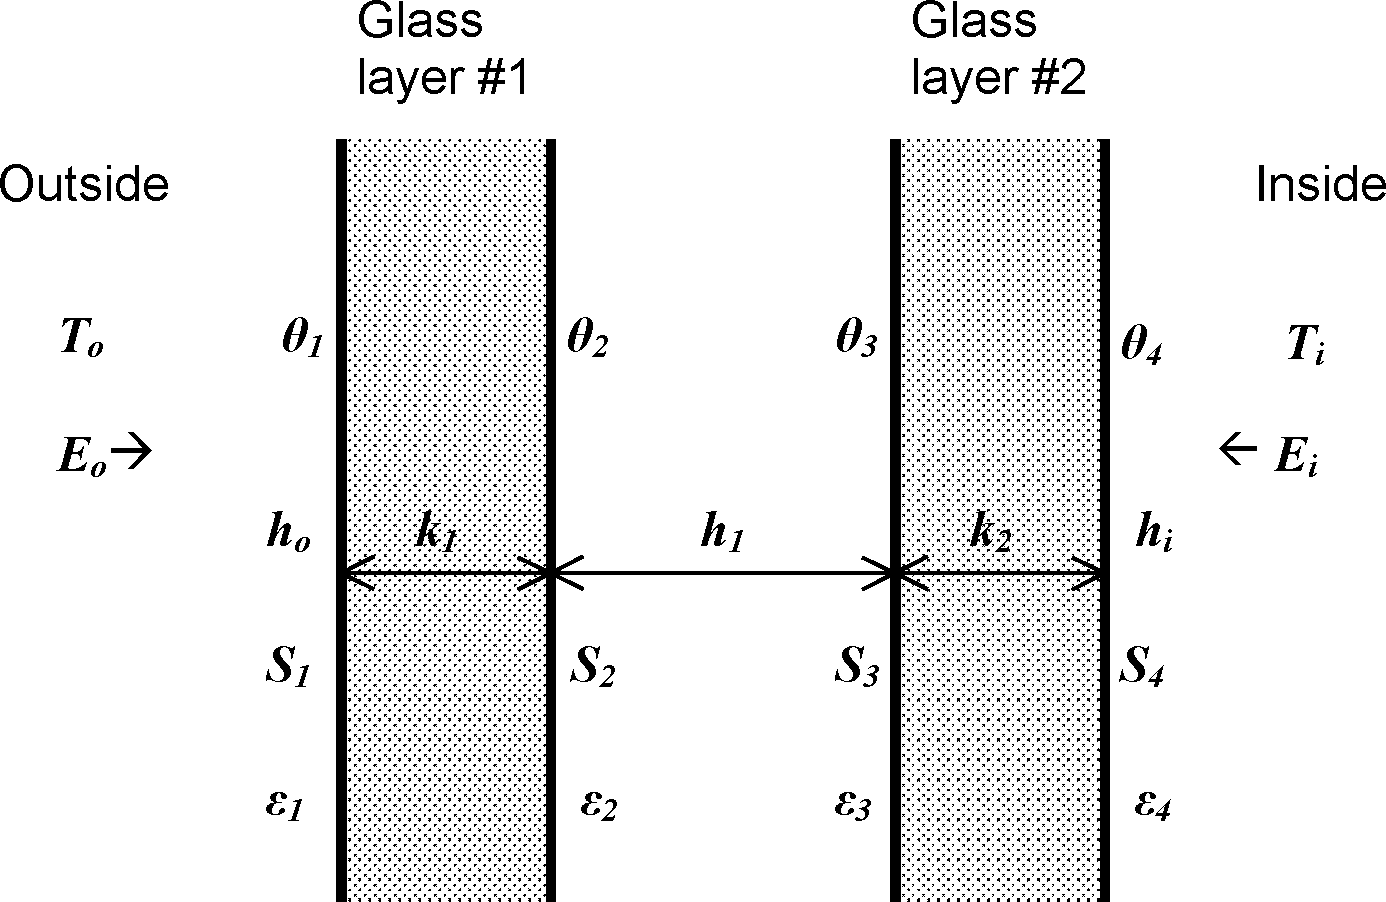
\includegraphics[width=0.9\textwidth, height=0.9\textheight, keepaspectratio=true]{media/image1470.png}
\caption{Glazing system with two glass layers showing variables used in heat balance equations. \protect \label{fig:glazing-system-with-two-glass-layers-showing}}
\end{figure}

The following assumptions are made in deriving the heat balance equations:

1)~~~~The glass layers are thin enough (a few millimeters) that heat storage in the glass can be neglected; therefore, there are no heat capacity terms in the equations.

2)~~~~The heat flow is perpendicular to the glass faces and is one dimensional. See ``Edge of Glass Corrections,'' below, for adjustments to the gap conduction in multi-pane glazing to account for 2-D conduction effects across the pane separators at the boundaries of the glazing.

3)~~~~The glass layers are opaque to IR. This is true for most glass products. For thin plastic suspended films this is not a good assumption, so the heat balance equations would have to be modified to handle this case.

4)~~~~The glass faces are isothermal. This is generally a good assumption since glass conductivity is very high.

5)~~~~The short wave radiation absorbed in a glass layer can be apportioned equally to the two faces of the layer.

The four equations for double-glazing are as follows. The equations for single glazing (\emph{N} = 1) and for \emph{N} = 3 and \emph{N} = 4 are analogous and are not shown.

\begin{equation}
{E_o}{\varepsilon_1} - {\varepsilon_1}\sigma \theta_1^4 + {k_1}\left( {{\theta_2} - {\theta_1}} \right) + {h_o}\left( {{T_o} - {\theta_1}} \right) + {S_1} = 0
\label{eq:GlazingFace1HeatBalEquation}
\end{equation}

\begin{equation}
{k_1}\left( {{\theta_1} - {\theta_2}} \right) + {h_1}\left( {{\theta_3} - {\theta_2}} \right) + \sigma \frac{{{\varepsilon_2}{\varepsilon_3}}}{{1 - \left( {1 - {\varepsilon_2}} \right)\left( {1 - {\varepsilon_3}} \right)}}\left( {\theta_3^4 - \theta_2^4} \right) + {S_2} = 0
\end{equation}

\begin{equation}
{h_1}({\theta_2} - {\theta_3}) + {k_2}({\theta_4} - {\theta_3}) + \sigma \frac{{{\varepsilon_2}{\varepsilon_3}}}{{1 - \left( {1 - {\varepsilon_2}} \right)\left( {1 - {\varepsilon_3}} \right)}}\left( {\theta_2^4 - \theta_3^4} \right) + {S_3} = 0
\end{equation}

\begin{equation}
{E_i}{\varepsilon_4} - {\varepsilon_4}\sigma \theta_4^4 + {k_2}\left( {{\theta_3} - {\theta_4}} \right) + {h_i}\left( {{T_i} - {\theta_4}} \right) + {S_4} = 0
\label{eq:GlazingFace4HeatBalEquation}
\end{equation}

\subsubsection{Absorbed Radiation}\label{absorbed-radiation}

\emph{S\(_{i}\)} in Equations~\ref{eq:GlazingFace1HeatBalEquation} to~\ref{eq:GlazingFace4HeatBalEquation} is the radiation (short-wave and long-wave from zone lights and equipment) absorbed on the \emph{i}\(^{th}\) face. Short-wave radiation (solar and short-wave from lights) is assumed to be absorbed uniformly along a glass layer, so for the purposes of the heat balance calculation it is split equally between the two faces of a layer. Glass layers are assumed to be opaque to IR so that the thermal radiation from lights and equipment is assigned only to the inside (room-side) face of the inside glass layer. For \emph{N} glass layers \emph{S\(_{i}\)} is given by

\begin{equation}
{S_{2j - 1}} = {S_{2j}} = \frac{1}{2}\left( {I_{bm}^{ext}\cos \phi A_j^f(\phi ) + I_{dif}^{ext}A_j^{f,dif} + I_{sw}^{{\mathop{\rm int}} }A_j^{b,dif}} \right),{\rm{    ~}}j = 1{\rm{~to~}}N
\end{equation}

\begin{equation}
{S_{2N}} = {S_{2N}} + {\varepsilon_{2N}}I_{lw}^{{\mathop{\rm int}} }
\end{equation}

Here

\(I_{bm}^{ext}\) = exterior beam normal solar irradiance

\(I_{dif}^{ext}\) = exterior diffuse solar incident on glazing from outside

\(I_{sw}^{{\mathop{\rm int}} }\) = interior short-wave radiation (from lights and from reflected diffuse solar) incident on glazing from inside

\(I_{lw}^{{\mathop{\rm int}} }\) = long-wave radiation from lights and equipment incident on glazing from inside

\({\varepsilon_{2N}}\) = emissivity (thermal absorptance) of the room-side face of the inside glass layer

\subsection{Room-Side Convection}\label{room-side-convection}

The correlation for room-side convection coefficient, \({h_i}\) , is from ISO 15099 section 8.3.2.2.~ (Prior to EnergyPlus version 3.1, the value for \({h_i}\) ~was modeled using the ``Detailed'' algorithm for opaque surface heat transfer, e.g.~for a vertical surface \({h_i} = 1.31{\left| {\Delta T} \right|^{{\raise0.7ex\hbox{1} \!\mathord{\left/ {\vphantom {1 3}}\right.}\!\lower0.7ex\hbox{3}}}}\) ; see section Detailed Natural Convection Algorithm).~ The ISO 15099 correlation is for still room air and is determined in terms of the Nusselt number, \(Nu\), is:

\begin{equation}
{h_i} = Nu\left( {\frac{\lambda }{H}} \right)
\end{equation}

where

\(\lambda\) ~is the thermal conductivity of air, and

\(H\) ~is the height of the window.

The Rayleigh number based on height, \(R{a_H}\) , is calculated using:

\begin{equation}
R{a_H} = \frac{{{\rho ^2}{H^3}g\,{c_p}\left| {{T_{surf,i}} - {T_{air}}} \right|}}{{{T_{m,f}}\mu \lambda }}
\end{equation}

where

\(\rho\) ~is the density of air

\(g\) ~is the acceleration due to gravity,

\({c_p}\) ~is the specific heat of air,

\(\mu\) ~is the dynamic viscosity of air, and

\({T_{m,f}}\) ~is the mean film temperature in Kelvin given by,

\begin{equation}
{T_{m,f}} = {T_{air}} + \frac{1}{4}\left( {{T_{surf,i}} - {T_{air}}} \right)
\end{equation}

There are four cases for the Nusselt correlation that vary by the tilt angle in degrees, \(\gamma\), and are based on heating conditions.~ For cooling conditions (where \({T_{surf,i}} > {T_{air}}\)), the tilt angle is complemented so that \(\gamma = 180 - \gamma\).

Case A. \({0^\circ } \le \gamma < 15^\circ\)

\begin{equation}
Nu = 0.13Ra_H^{{\raise0.7ex\hbox{1} \!\mathord{\left/ {\vphantom {1 3}}\right.}\!\lower0.7ex\hbox{3}}}
\end{equation}

Case B. \(15^\circ \le \gamma \le 90^\circ\)

\begin{equation}
R{a_{cv}} = 2.5 \times {10^5}{\left( {\frac{{{e^{0.72\gamma }}}}{{\sin \lambda }}} \right)^{{\raise0.7ex\hbox{1} \!\mathord{\left/ {\vphantom {1 5}}\right.}\!\lower0.7ex\hbox{5}}}}
\end{equation}

\begin{equation}
Nu = 0.56{\left( {R{a_H}\sin \gamma } \right)^{{\raise0.7ex\hbox{1} \!\mathord{\left/ {\vphantom {1 4}}\right.}\!\lower0.7ex\hbox{4}}}};\;for\;R{a_H} \le R{a_{CV}}
\end{equation}

\begin{equation}
Nu = 0.13\left( {Ra_H^{{\raise0.7ex\hbox{1} \!\mathord{\left/ {\vphantom {1 3}}\right.}\!\lower0.7ex\hbox{3}}} - Ra_{CV}^{{\raise0.7ex\hbox{1} \!\mathord{\left/ {\vphantom {1 3}}\right.}\!\lower0.7ex\hbox{3}}}} \right) + 0.56{\left( {R{a_{CV}}\sin \gamma } \right)^{{\raise0.7ex\hbox{1} \!\mathord{\left/ {\vphantom {1 4}}\right.}\!\lower0.7ex\hbox{4}}}};\;R{a_H} > R{a_{CV}}
\end{equation}

Case C. \(90^\circ < \gamma \le 179^\circ\)

\begin{equation}
Nu = 0.56{\left( {R{a_H}\sin \gamma } \right)^{{\raise0.7ex\hbox{1} \!\mathord{\left/ {\vphantom {1 4}}\right.}\!\lower0.7ex\hbox{4}}}};\;{10^5} \le R{a_H}\sin \gamma  < {10^{11}}
\end{equation}

Case D. \(179^\circ < \gamma \le 180^\circ\)

\begin{equation}
Nu = 0.58Ra_H^{{\raise0.7ex\hbox{1} \!\mathord{\left/ {\vphantom {1 5}}\right.}\!\lower0.7ex\hbox{5}}};\;R{a_H} \le {10^{11}}
\end{equation}

The material properties are evaluated at the mean film temperature.~ Standard EnergyPlus pyschrometric functions are used for \(\rho\) ~and \({c_p}\).~ Thermal conductivity is calculated using:

\begin{equation}
\lambda = 2.873 \times {10^{ - 3}} + 7.76 \times {10^{ - 5}}{T_{m,f}}
\end{equation}

Kinematic viscosity is calculated using:

\begin{equation}
\mu = 3.723 \times {10^{ - 6}} + 4.94 \times {10^{ - 8}}{T_{m,f}}
\end{equation}

This correlation depends on the surface temperature of the room-side glazing surface and is therefore included inside the window heat balance interation loop.

\subsection{Solving the Glazing Heat Balance Equations}\label{solving-the-glazing-heat-balance-equations}

The equations are solved as follows:

1)~~~~Linearize the equations by defining \({h_{r,i}} = {\varepsilon_i}\sigma \theta_i^3\) .~ For example, Equation~\ref{eq:GlazingFace1HeatBalEquation} becomes

\begin{equation}
{E_o}{\varepsilon_1} - {h_{r,1}}{\theta_1} + {k_1}\left( {{\theta_2} - {\theta_1}} \right) + {h_o}\left( {{T_o} - {\theta_1}} \right) + {S_1} = 0
\end{equation}

2)~~~~Write the equations in the matrix form \(A\theta = B\)

3)~~~~Use previous time step's values of \({\theta_i}\) as initial values for the current time step. For the first time step of a design day or run period the initial values are estimated by treating the layers as a simple RC network.

4)~~~~Save the \({\theta_i}\) for use in the next iteration: \({\theta_{prev,i}} = {\theta_i}\)

5)~~~~Using \({\theta_{2N}}\), reevaluate the room-side face surface convection coefficient \({h_i}\)

6)~~~~Using the \({\theta_i}\)~to evaluate the radiative conductances \({h_{r,i}}\)

7)~~~~Find the solution \(\theta = {A^{ - 1}}B\) by LU decomposition

8)~~~~Perform relaxation on the the new \({\theta_i}\) \textbf{:} \({\theta_i} \to \left( {{\theta_i} + {\theta_{prev,i}}} \right)/2\)

9)~~~~Go to step 4

Repeat steps 4 to 9 until the difference, \(\Delta {\theta_i}\), between values of the \({\theta_i}\)~in successive iterations is less than some tolerance value. Currently, the test is:

\begin{equation}
\frac{1}{{2N}}\sum\limits_{i = 1}^{2N} {|\Delta {\theta_i}|{\rm{ }} < 0.02K}
\end{equation}

If this test does not pass after 100 iterations, the tolerance is increased to 0.2K. If the test still fails the program stops and an error message is issued.

The value of the inside face temperature, \({\theta_{2N}}\), determined in this way participates in the zone heat balance solution (see Outdoor/Exterior Convection) and thermal comfort calculation (see Occupant Thermal Comfort).

\subsection{Edge-Of-Glass Effects}\label{edge-of-glass-effects}

% table 37
\begin{longtable}[c]{p{1.0in}p{2.5in}p{1.0in}p{1.5in}}
\caption{C++ Variables used in Edge of Glass calculations \label{table:c++-variables-used-in-edge-of-glass}} \tabularnewline
\toprule 
Mathematical variable & Description & Units & C++ variable \tabularnewline
\midrule
\endfirsthead

\caption[]{C++ Variables used in Edge of Glass calculations} \tabularnewline
\toprule 
Mathematical variable & Description & Units & C++ variable \tabularnewline
\midrule
\endhead

\(\overline h\) & Area-weighted net conductance of glazing including edge-of-glass effects & W/m\(^{2}\)-K & - \tabularnewline
A\(_{cg}\) & Area of center-of-glass region & m\(^{2}\) & CenterGlArea \tabularnewline
A\(_{fe}\) & Area of frame edge region & m\(^{2}\) & FrameEdgeArea \tabularnewline
A\(_{de}\) & Area of divider edge region & m\(^{2}\) & DividerEdgeArea \tabularnewline
A\(_{tot}\) & Total glazing area & m\(^{2}\) & Surface\%Area \tabularnewline
h\(_{cg}\) & Conductance of center-of-glass region (without air films) & W/m\(^{2}\)-K & - \tabularnewline
h\(_{fe}\) & Conductance of frame edge region (without air films) & W/m\(^{2}\)-K & - \tabularnewline
h\(_{de}\) & Conductance of divider edge region (without air films) & W/m\(^{2}\)-K & - \tabularnewline
h\(_{ck}\) & Convective conductance of gap k & W/m\(^{2}\)-K & - \tabularnewline
h\(_{rk}\) & Radiative conductance of gap k & W/m\(^{2}\)-K & - \tabularnewline
$\eta$ & Area ratio & - & - \tabularnewline
$\alpha$ & Conductance ratio & - & FrEdgeToCenterGlCondRatio, DivEdgeToCenterGlCondRatio \tabularnewline
\bottomrule
\end{longtable}

Because of thermal bridging across the spacer separating the glass layers in multi-pane glazing, the conductance of the glazing near the frame and divider, where the spacers are located, is higher than it is in the center of the glass. The area-weighted net conductance (without inside and outside air films) of the glazing in this case can be written

\begin{equation}
\overline h  = \left( {{A_{cg}}{h_{cg}} + {A_{fe}}{h_{fe}} + {A_{de}}{h_{de}}} \right)/{A_{tot}}
\label{eq:AreaWeightedNetConductance}
\end{equation}

where

\emph{h\(_{cg}\)} = conductance of center-of-glass region (without air films)

\emph{h\(_{fe}\)} = conductance of frame edge region (without air films)

\emph{h\(_{de}\)} = conductance of divider edge region (without air films)

\emph{A\(_{cg}\)} = area of center-of-glass region

\emph{A\(_{fe}\)} = area of frame edge region

\emph{A\(_{de}\)} = area of divider edge region

\emph{A\(_{tot}\)} = total glazing area = \({A_{cg}} + {A_{fe}} + {A_{de}}\)

The different regions are shown in Figure~\ref{fig:different-types-of-glass-regions.}:

\begin{figure}[hbtp] % fig 96
\centering
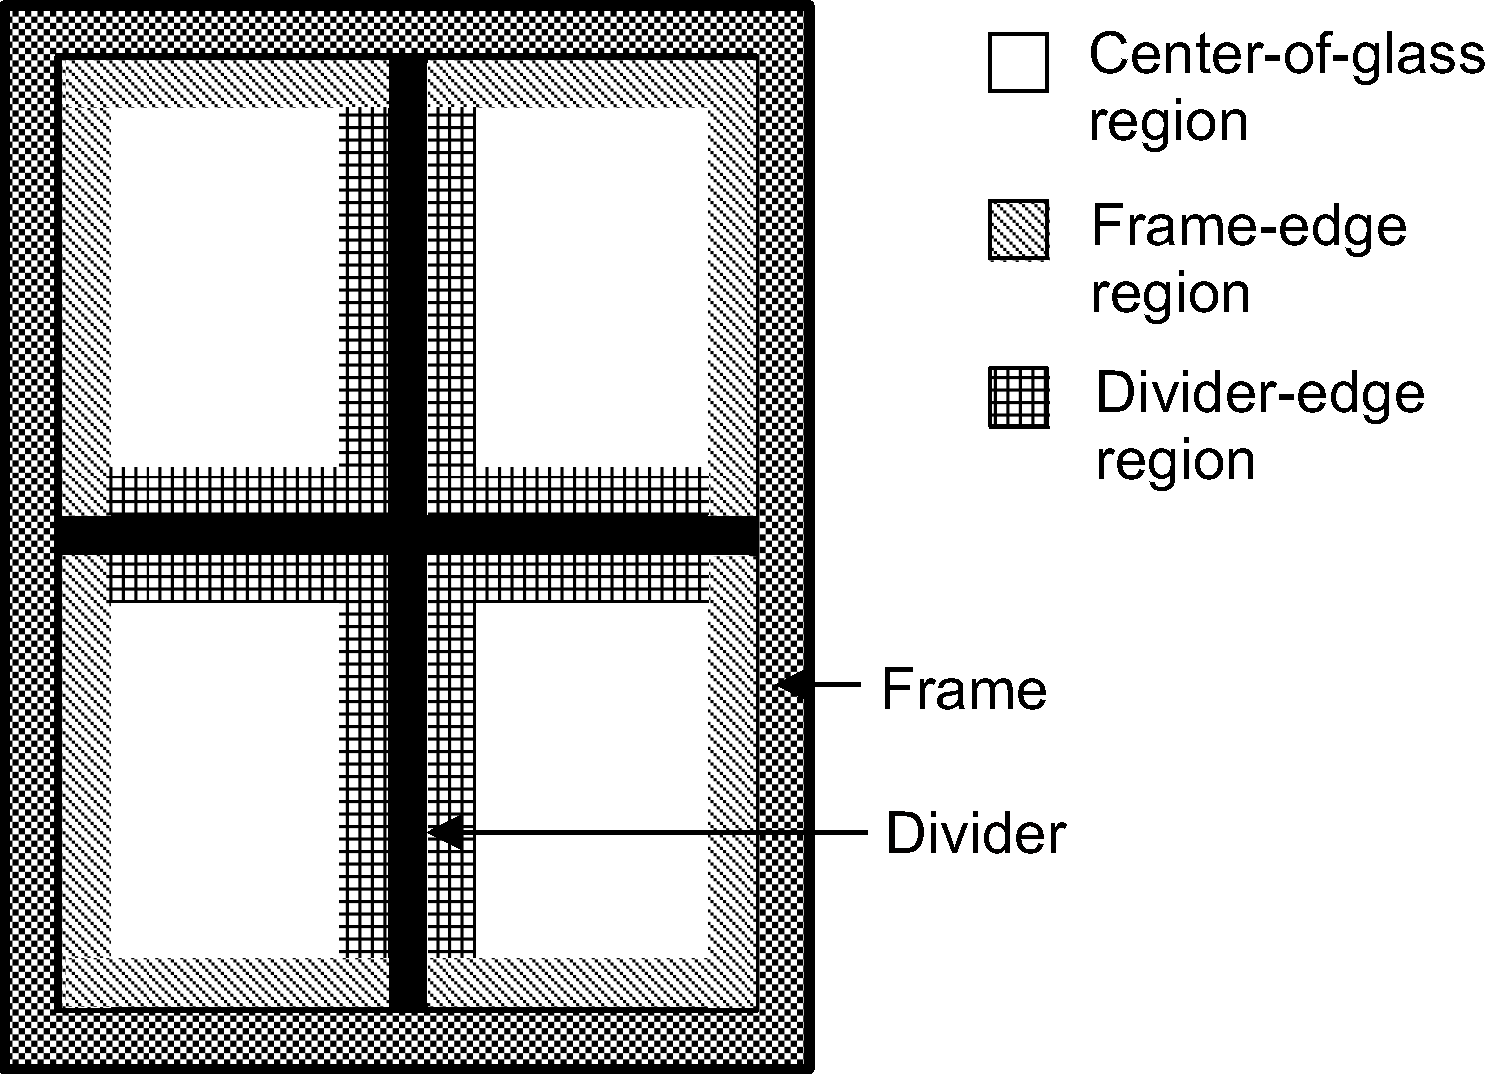
\includegraphics[width=0.9\textwidth, height=0.9\textheight, keepaspectratio=true]{media/image1534.png}
\caption{Different types of glass regions. \label{fig:different-types-of-glass-regions.}}
\end{figure}

Equation~\ref{eq:AreaWeightedNetConductance} can be rewritten as:

\begin{equation}
\overline h  = {h_{cg}}\left( {{\eta_{cg}} + {\alpha_{fe}}{\eta_{fe}} + {\alpha_{de}}{\eta_{de}}} \right)
\label{eq:HbarConductanceEquation}
\end{equation}

where

\begin{equation}
{\eta_{cg}} = {A_{cg}}/{A_{tot}}
\end{equation}

\begin{equation}
{\eta_{fe}} = {A_{fe}}/{A_{tot}}
\end{equation}

\begin{equation}
{\eta_{de}} = {A_{de}}/{A_{tot}}
\end{equation}

\begin{equation}
{\alpha_{fe}} = {h_{fe}}/{h_{cg}}
\end{equation}

\begin{equation}
{\alpha_{de}} = {h_{de}}/{h_{cg}}
\end{equation}

The conductance ratios \({\alpha_{fe}}\) ~and \({\alpha_{de}}\) are user inputs obtained from Window 5. They depend on the glazing construction as well as the spacer type, gap width, and frame and divider type.

In the EnergyPlus glazing heat balance calculation effective gap convective conductances are used to account for the edge-of-glass effects. These effective conductances are determined as follows for the case with two gaps (triple glazing). The approach for other numbers of gaps is analogous.

Neglecting the very small resistance of the glass layers, the center-of-glass conductance (without inside and outside air films) can be written as:

\begin{equation}
{h_{cg}} = {\left( {{{\left( {{h_{r,1}} + {h_{c,1}}} \right)}^{ - 1}} + {{\left( {{h_{r,2}} + {h_{c,2}}} \right)}^{ - 1}}} \right)^{ - 1}}
\end{equation}

where

\emph{h\(_{c,k}\)} = convective conductance of the \emph{k\(^{h}\)} gap

\emph{h\(_{r,k}\)} = radiative conductance of the \emph{k\(^{h}\)} gap or:

\begin{equation}
h_{r,k}= \frac{1}{2}\sigma \frac{{{\varepsilon_i}{\varepsilon_j}}}{{1 - \left( {1 - {\varepsilon_i}} \right)\left( {1 - {\varepsilon_j}} \right)}}{\left( {{\theta_i} + {\theta_j}} \right)^3}
\end{equation}

$\varepsilon$\(_{i}\), $\varepsilon$\(_{j}\) = emissivity of the faces bounding the gap

$\theta$\(_{i}\), $\theta$\(_{j}\) = temperature of faces bounding the gap (K)

Equation~\ref{eq:HbarConductanceEquation} then becomes:

\begin{equation}
\overline h  = \left( {{\eta_{cg}} + {\alpha_{fe}}{\eta_{fe}} + {\alpha_{de}}{\eta_{de}}} \right){\left( {{{\left( {{h_{r,1}} + {h_{c,1}}} \right)}^{ - 1}} + {{\left( {{h_{r,2}} + {h_{c,2}}} \right)}^{ - 1}}} \right)^{ - 1}}
\label{eq:HbarwithetaalphaEquation}
\end{equation}

We can also write \(\overline h\) in terms of effective convective conductances of the gaps as:

\begin{equation}
\overline h  = {\left( {{{\left( {{h_{r,1}} + {{\overline h }_{c,1}}} \right)}^{ - 1}} + {{\left( {{h_{r,2}} + {{\overline h }_{c,2}}} \right)}^{ - 1}}} \right)^{ - 1}}
\label{eq:HbarwithhrandhcEquation}
\end{equation}

Comparing Equations~\ref{eq:HbarwithetaalphaEquation} and~\ref{eq:HbarwithhrandhcEquation}, we obtain:

\begin{equation}
{h_{r,k}} + {\overline h_{c,k}} = \left( {{\eta_{cg}} + {\alpha_{fe}}{\eta_{fe}} + {\alpha_{de}}{\eta_{de}}} \right)\left( {{h_{r,k}} + {h_{c,k}}} \right)
\end{equation}

Using \({\eta_{cg}} = 1 - {\eta_{fe}} - {\eta_{de}}\)~gives:

\begin{equation}
{\overline h_{c,k}} = {h_{r,k}}\left( {{\eta_{fe}}\left( {{\alpha_{fe}} - 1} \right) + {\eta_{de}}\left( {{\alpha_{de}} - 1} \right)} \right) + {h_{c,k}}\left( {1 + {\eta_{fe}}\left( {{\alpha_{fe}} - 1} \right) + {\eta_{de}}\left( {{\alpha_{de}} - 1} \right)} \right)
\end{equation}

This is the expression used by EnergyPlus for the gap convective conductance when a frame or divider is present.

\subsection{Apportioning of Absorbed Short-Wave Radiation in Shading Device Layers}\label{apportioning-of-absorbed-short-wave-radiation-in-shading-device-layers}

If a shading device has a non-zero short-wave transmittance then absorption takes place throughout the shading device layer. The following algorithm is used to apportion the absorbed short-wave radiation to the two faces of the layer. Here \emph{f\(_{1}\)} is the fraction assigned to the face closest to the incident radiation and \emph{f\(_{2}\)} is the fraction assigned to the face furthest from the incident radiation.

\begin{equation}
{f_1} = 1,~{\rm{ }}{f_2} = 0{\rm{~if~}}{\tau_{sh}} = 0
\end{equation}

Otherwise:

\begin{equation}
  \begin{array}{cl}
    f_1 = 0,\;f_2 = 0 &\text{if~} \alpha_{sh} \le 0.01 \\
    f_1 = 1,\;f_2 = 0 &\text{if~} \alpha_{sh} > 0.999 \\
    \left.
      \begin{array}{l}
        f_1 = \frac{1 - e^{0.5 \ln (1 - \alpha_{sh})}} {\alpha_{sh}} \\
        f_2 = 1 - {f_1}
      \end{array}
    \right\} &\text{if~} 0.01 < \alpha_{sh} \le 0.999
  \end{array}
\end{equation}

\subsection{Window~ Frame and Divider Calculation}\label{window-frame-and-divider-calculation}

For the zone heat balance calculation the inside surface temperature of the frame and that of the divider are needed. These temperatures are determined by solving the heat balance equations on the inside and outside surfaces of the frame and divider.

% table 38
\begin{longtable}[c]{p{1.0in}p{2.5in}p{1.0in}p{1.5in}}
\caption{C++ Variables used in Window/Frame and Divider calculations \label{table:c++-variables-used-in-windowframe}} \tabularnewline
\toprule 
Mathematical variable & Description & Units & C++ variable \tabularnewline
\midrule
\endfirsthead

\caption[]{C++ Variables used in Window/Frame and Divider calculations} \tabularnewline
\toprule 
Mathematical variable & Description & Units & C++ variable \tabularnewline
\midrule
\endhead

Q\(_{ExtIR,abs}\) & IR from the exterior surround absorbed by outside frame surfaces & W & - \tabularnewline
Q\(_{IR,emitted}\) & IR emitted by outside frame surfaces & W & - \tabularnewline
Q\(_{conv}\) & Convection from outside air to outside frame surfaces & W & - \tabularnewline
Q\(_{cond}\) & Conduction through frame from inside frame surfaces to outside frame surfaces & W & - \tabularnewline
Q\(_{abs}\) & Solar radiation plus outside glass IR absorbed by outside of frame & W & - \tabularnewline
Q\(^{dif}_{abs,sol}\) & Diffuse solar absorbed by outside frame surfaces, per unit frame face area & W/m\(^{2}\) & - \tabularnewline
Q\(^{bm}_{abs,sol}\) & Beam solar absorbed by outside frame surfaces, per unit frame face area & W/m\(^{2}\) & - \tabularnewline
I\(^{dif}_{ext}\) & Diffuse solar incident on window & W/m\(^{2}\) & - \tabularnewline
I\(^{bm}_{ext}\) & Direct normal solar irradiance & W/m\(^{2}\) & - \tabularnewline
$\alpha$\(^{fr}_{sol}\) & Solar absorptance of frame & - & FrameSolAbsorp \tabularnewline
R\(_{gl}^{f,dif}\) & Front diffuse solar reflectance of glazing & - & ~ \tabularnewline
R\(_{gl}^{f,bm}\) & Front beam solar reflectance of glazing & - & ~ \tabularnewline
cos($\beta$\(_{face}\)) & Cosine of angle of incidence of beam solar on frame outside face & ~ & CosIncAng \tabularnewline
cos($\beta$\(_{h}\)) & Cosine of angle of incidence of beam solar on frame projection parallel to window x-axis & - & CosIncAngHorProj \tabularnewline
cos($\beta$\(_{v}\)) & Cosine of angle of incidence of beam solar on frame projection parallel to window y-axis & - & CosIncAngVertProj \tabularnewline
f\(_{sunlight}\) & Fraction of window that is sunlit & - & SunlitFrac \tabularnewline
A\(_{f}\) & Area of frame’s outside face (same as area of frame’s inside face) & m\(^{2}\) & - \tabularnewline
A\(_{p1}\), A\(_{p2}\) & Area of frame’s outside and inside projection faces & m\(^{2}\) & - \tabularnewline
F\(_{f}\) & Form factor of frame’s outside or inside face for IR & - & - \tabularnewline
F\(_{p1}\), F\(_{p2}\) & Form factor of frame outside projection for exterior IR; form factor of frame inside projection for interior IR & - & - \tabularnewline
E\(_{o}\) & Exterior IR incident on window plane & W/m\(^{2}\) & outir \tabularnewline
E\(_{i}\) & Interior IR incident on window plane & W/m\(^{2}\) & SurroundIRfromParentZone \tabularnewline
$\varepsilon$\(_{1}\), $\varepsilon$\(_{2}\) & Outside, inside frame surface emissivity & - & FrameEmis \tabularnewline
$\theta$\(_{1}\), $\theta$\(_{2}\) & Frame outside, inside surface temperature & K & FrameTempSurfOut, FrameSurfTempIn \tabularnewline
T\(_{o}\), T\(_{i}\) & Outdoor and indoor air temperatures & K & tout, tin \tabularnewline
h\(_{o,c}\), h\(_{i,c}\) & Frame outside and inside air film convective conductance & W/m\(^{2}\)-K & HOutConv, HInConv \tabularnewline
k & Effective inside-surface to outside-surface conductance of frame per unit area of frame projected onto window plane & W/m\(^{2}\)-K & FrameConductance, FrameCon \tabularnewline
S\(_{1}\) & Q\(_{abs}\)/A\(_{f}\) & W/m\(^{2}\)-K & FrameQRadOutAbs \tabularnewline
S\(_{2}\) & Interior short-wave radiation plus interior IR from internal sources absorbed by inside of frame divided by A\(_{f}\) & W/m\(^{2}\)-K & FrameQRadInAbs \tabularnewline
$\eta$\(_{1}\), $\eta$\(_{2}\) & A\(_{p1}\)/A\(_{f}\), A\(_{p2}\)/A\(_{f}\) & - & - \tabularnewline
H & Height of glazed portion of window & m & Surface\%Height \tabularnewline
W & Width of glazed portion of window & m & Surface\%Width \tabularnewline
w\(_{f}\), w\(_{d}\) & Frame width, divider width & m & FrameWidth, DividerWidth \tabularnewline
p\(_{f1}\), p\(_{f2}\) & Frame outside, inside projection & m & FrameProjectionOut, FrameProjectionIn \tabularnewline
N\(_{h}\), N\(_{v}\) & Number of horizontal, vertical dividers & - & HorDividers, VertDividers \tabularnewline
T\(_{o,r}\), T\(_{i,r}\) & Frame outside, inside radiative temperature & K & TOutRadFr, TInRadFr \tabularnewline
h\(_{o,r}\), h\(_{i,r}\) & Frame outside, inside surface radiative conductance & W/m\(^{2}\)-K & HOutRad, HInRad \tabularnewline
A & Intermediate variable in frame heat balance solution & K & Afac \tabularnewline
C & Intermediate variable in frame heat balance solution & - & Efac \tabularnewline
B, D & Intermediate variables in frame heat balance solution & - & Bfac, Dfac \tabularnewline
\bottomrule
\end{longtable}

\subsubsection{Frame Temperature Calculation}\label{frame-temperature-calculation}

Figure~\ref{fig:cross-section-through-a-window-showing-frame} shows a cross section through a window showing frame and divider. The outside and inside frame and divider surfaces are assumed to be isothermal. The frame and divider profiles are approximated as rectangular since this simplifies calculating heat gains and losses (see ``Error Due to Assuming a Rectangular Profile,'' below).

\begin{figure}[hbtp] % fig 97
\centering
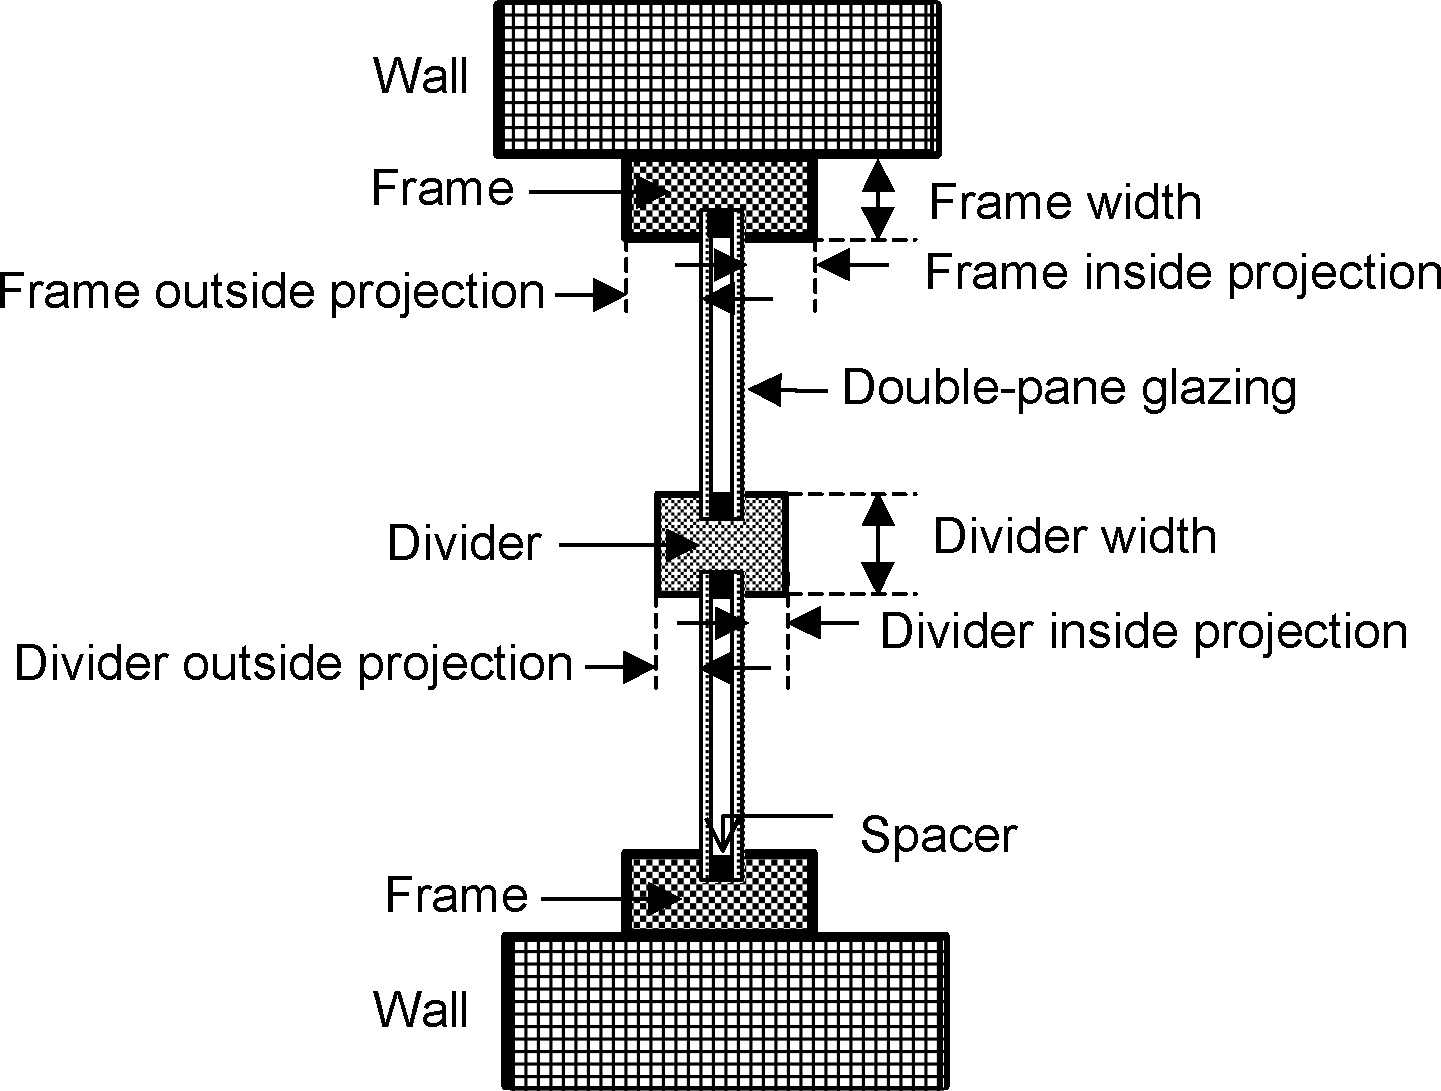
\includegraphics[width=0.9\textwidth, height=0.9\textheight, keepaspectratio=true]{media/image1557.png}
\caption{Cross section through a window showing frame and divider (exaggerated horizontally). \label{fig:cross-section-through-a-window-showing-frame}}
\end{figure}

\textbf{~}

\subsubsection{Frame Outside Surface Heat Balance}\label{frame-outside-surface-heat-balance}

The outside surface heat balance equation is:

\begin{equation}
{Q_{ExtIR,abs}} - {Q_{IR,emitted}} + {Q_{conv}} + {Q_{cond}} + {Q_{abs}} = 0
\end{equation}

where

\({Q_{ExtIR,abs}}\) ~ = IR from the exterior surround (sky and ground) absorbed by outside frame surfaces

\({Q_{IR,emitted}}\) = IR emitted by outside frame surfaces

\({Q_{conv}}\) = convection from outside air to outside frame surfaces

\({Q_{cond}}\) = conduction through frame from inside frame surfaces to outside frame surfaces

\({Q_{abs}}\) = solar radiation (from sun, sky and ground) plus IR from outside window surface absorbed by outside frame surfaces (see ``Calculation of Absorbed Solar Radiation,'' below).

The first term can be written as the sum of the exterior IR absorbed by the outside face of the frame and the exterior IR absorbed by the frame's outside projection surfaces.

\begin{equation}
{Q_{ExtIR,abs}} = {\varepsilon_1}{E_o}{A_f}{F_f} + {\varepsilon_1}{E_o}{A_{p1}}{F_{p1}}
\end{equation}

where \emph{\(\varepsilon\)\(_{1}\)} is the outside surface emissivity.

The exterior IR incident on the plane of the window, \emph{E\(_{o}\)}, is the sum of the IR from the sky, ground and obstructions. For the purposes of the frame heat balance calculation it is assumed to be isotropic. For isotropic incident IR, \emph{F\(_{f}\)} = 1.0 and \emph{F\(_{p1}\)} = 0.5, which gives:

\begin{equation}
{Q_{ExtIR,abs}} = {\varepsilon_1}{E_o}({A_f} + \frac{1}{2}{A_{p1}})
\end{equation}

The IR emitted by the outside frame surfaces is:

\begin{equation}
{Q_{ExtIR,emitted}} = {\varepsilon_1}\sigma ({A_f} + {A_{p1}})\theta_1^4
\end{equation}

The convective heat flow from the outside air to the outside frame surfaces is:

\begin{equation}
{Q_{conv}} = {h_{o,c}}({A_f} + {A_{p1}})({T_o} - {\theta_1})
\end{equation}

The conduction through the frame from inside to outside is:

\begin{equation}
{Q_{cond}} = k{A_f}({\theta_2} - {\theta_1})
\end{equation}

Note that \emph{A\(_{f}\)}~is used here since the conductance, \emph{k}, is, by definition, per unit area of frame projected onto the plane of the window.

Adding these expressions for the \emph{Q} terms and dividing by A\(_{f}\)~gives:

\begin{equation}
{E_0}{\varepsilon_1}\left( {1 + \frac{1}{2}{\eta_1}} \right) - {\varepsilon_1}\left( {1 + {\eta_1}} \right)\theta_1^4 + {h_{o,c}}\left( {1 + {\eta_1}} \right)\left( {{T_0} - {\theta_1}} \right) + k\left( {{\theta_2} - {\theta_1}} \right) + {S_1} = 0
\label{eq:E0epsilon1Equation}
\end{equation}

where \emph{S\(_{1}\)} = \emph{Q\(_{abs}\)/A\(_{f}\)}~and

\begin{equation}
{\eta_1} = \frac{{{A_{p1}}}}{{{A_f}}} = \left( {\frac{{{p_{f,1}}}}{{{w_f}}}} \right)\frac{{H + W - ({N_h} + {N_v}){w_d}}}{{H + W + 2{w_f}}}
\end{equation}

We linearize Equation~\ref{eq:E0epsilon1Equation} as follows.  Write the first two terms as:

\begin{equation}
{\varepsilon_1}(1 + {\eta_1})[{E_o}(1 + \frac{1}{2}{\eta_1})/(1 + {\eta_1}) - \theta_1^4]
\end{equation}

and define a radiative temperature:

\begin{equation}
{T_{o,r}} = {[{E_o}(1 + \frac{1}{2}{\eta_1})/(1 + {\eta_1})]^{1/4}}
\end{equation}

This gives:

\begin{equation}
{\varepsilon_1}(1 + {\eta_1})[T_{o,r}^4 - \theta_1^4]
\end{equation}

which, within a few percent, equals:

\begin{equation}
{\varepsilon_1}(1 + {\eta_1})\frac{{{{({T_{o,r}} + {\theta_1})}^3}}}{2}({T_{o,r}} - {\theta_1})
\end{equation}

Defining an outside surface radiative conductance as follows:

\begin{equation}
{h_{o,r}} = {\varepsilon_1}(1 + {\eta_1})\frac{{{{({T_{o,r}} + {\theta_1})}^3}}}{2}
\end{equation}

then gives:

\begin{equation}
{h_{o,r}}({T_{o,r}} - {\theta_1})
\end{equation}

The final outside surface heat balance equation in linearized form is then:

\begin{equation}
{h_{o,r}}({T_{o,r}} - {\theta_1}) + {h_{o,c}}(1 + {\eta_1})({T_o} - {\theta_1}) + k({\theta_2} - {\theta_1}) + {S_1} = 0
\label{eq:horEquation}
\end{equation}

\subsubsection{Frame Inside Surface Heat Balance}\label{frame-inside-surface-heat-balance}

A similar approach can be used to obtain the following linearized \emph{inside} surface heat balance equation:

\begin{equation}
{h_{i,r}}({T_{i,r}} - {\theta_2}) + {h_{i,c}}(1 + {\eta_2})({T_i} - {\theta_2}) + k({\theta_1} - {\theta_2}) + {S_2} = 0
\label{eq:hirEquation}
\end{equation}

where

\begin{equation}
{T_{i,r}} = {[{E_i}(1 + \frac{1}{2}{\eta_2})/(1 + {\eta_2})]^{1/4}}
\end{equation}

\begin{equation}
{\eta_2} = \frac{{{A_{p2}}}}{{{A_f}}} = \left( {\frac{{{p_{f,2}}}}{{{w_f}}}} \right)\frac{{H + W - ({N_h} + {N_v}){w_d}}}{{H + W + 2{w_f}}}
\end{equation}

and \emph{E\(_{i}\)} is the interior IR irradiance incident on the plane of the window.

Solving Equations~\ref{eq:horEquation} and~\ref{eq:hirEquation} simultaneously gives:

\begin{equation}
{\theta_2} = \frac{{D + CA}}{{1 - CB}}
\end{equation}

with

\begin{equation}
A = \frac{{{h_{o,r}}{T_{o,r}} + {h_{o,c}}{T_o} + {S_1}}}{{{h_{o,r}} + k + {h_{o,c}}}}
\end{equation}

\begin{equation}
B = \frac{k}{{{h_{o,r}} + k + {h_{o,c}}}}
\end{equation}

\begin{equation}
C = \frac{k}{{{h_{i,r}} + k + {h_{i,c}}}}
\end{equation}

\begin{equation}
D = \frac{{{h_{i,r}}{T_{i,r}} + {h_{i,c}}{T_i} + {S_2}}}{{{h_{i,r}} + k + {h_{i,c}}}}
\end{equation}

\subsubsection{Calculation of Solar Radiation Absorbed by Frame}\label{calculation-of-solar-radiation-absorbed-by-frame}

The frame outside face and outside projections and inside projections absorb beam solar radiation (if sunlight is striking the window) and diffuse solar radiation from the sky and ground. For the outside surfaces of the frame, the absorbed diffuse solar per unit frame face area is:

\begin{equation}
Q_{abs,sol}^{dif} = I_{ext}^{dif}{\alpha_{fr,sol}}\left( {{A_f} + {F_{p1}}{A_{p1}}} \right)/{A_f} = I_{ext}^{dif}{\alpha_{fr,sol}}\left( {1 + 0.5\frac{{{A_{p1}}}}{{{A_f}}}} \right)
\end{equation}

If there is no exterior window shade, \emph{~I\(^{dif}\)\(_{ext}\)} includes the effect of diffuse solar reflecting off of the glazing onto the outside frame projection, i.e.,

\begin{equation}
I_{ext}^{dif} \to I_{ext}^{dif}\left( {1 + R_{gl}^{f,dif}} \right)
\end{equation}

The beam solar absorbed by the outside face of the frame, per unit frame face area is:

\begin{equation}
Q_{abs,sol}^{bm,face} = I_{ext}^{bm}{\alpha_{fr,sol}}\cos {\beta_{face}}{f_{sunlit}}
\end{equation}

The beam solar absorbed by the frame outside projection parallel to the window x-axis is:

\begin{equation}
Q_{abs,sol}^{bm,h} = I_{ext}^{bm}{\alpha_{fr,sol}}\cos {\beta_h}{p_{f1}}\left( {W - {N_v}{w_d}} \right){f_{sunlit}}/{A_f}
\end{equation}

Here it is assumed that the sunlit fraction, \emph{f\(_{sunlit}\)}, for the window can be applied to the window frame. Note that at any given time beam solar can strike only one of the two projection surfaces that are parallel to the window x-axis. If there is no exterior window shade, \emph{I\(^{bm}\)\(_{ext}\)} includes the effect of beam solar reflecting off of the glazing onto the outside frame projection, i.e.,

\begin{equation}
I_{ext}^{bm} \to I_{ext}^{bm}\left( {1 + R_{gl}^{f,bm}} \right)
\end{equation}

The beam solar absorbed by the frame outside projection parallel to the window y-axis is:

\begin{equation}
Q_{abs,sol}^{bm,v} = I_{ext}^{bm}{\alpha_{fr,sol}}\cos {\beta_v}{p_{f1}}\left( {H - {N_h}{w_d}} \right){f_{sunlit}}/{A_f}
\end{equation}

Using a similar approach, the beam and diffuse solar absorbed by the \emph{inside} frame projections is calculated, taking the transmittance of the glazing into account.

\subsubsection{Error Due to Assuming a Rectangular Profile}\label{error-due-to-assuming-a-rectangular-profile}

Assuming that the inside and outside frame profile is rectangular introduces an error in the surface heat transfer calculation if the profile is non-rectangular. The percent error in the calculation of convection and emitted IR is approximately 100\(\left| {{L_{profile,rect}} - {L_{profile,actual}}} \right|/{L_{profile,rect}}\), where \emph{L\(_{profile,rect}\)} is the profile length for a rectangular profile (\emph{w\(_{f}\)} + p\(_{f1}\) for outside of frame or \emph{w\(_{f}\)} + \emph{p\(_{f2}\)} for inside of frame) and \emph{L\(_{profile,actual}\)} is the actual profile length. For example, for a circular profile \emph{vs} a square profile the error is about 22\%. The error in the calculation of absorbed beam radiation is close to zero since the beam radiation intercepted by the profile is insensitive to the shape of the profile. The error in the absorbed diffuse radiation and absorbed IR depends on details of the shape of the profile. For example, for a circular profile vs.~a square profile the error is about 15\%.

\subsubsection{Divider Temperature Calculation}\label{divider-temperature-calculation}

The divider inside and outside surface temperatures are determined by a heat balance calculation that is analogous to the frame heat balance calculation described above.

\subsection{Beam Solar Reflection from Window Reveal Surfaces}\label{beam-solar-reflection-from-window-reveal-surfaces}

This section describes how beam solar radiation that is reflected from window reveal surfaces is calculated. Reflection from outside reveal surfaces---which are associated with the setback of the glazing from the outside surface of the window's parent wall---increases the solar gain through the glazing. Reflection from inside reveal surfaces---which are associated with the setback of the glazing from the inside surface of the window's parent wall---decreases the solar gain to the zone because some of this radiation is reflected back out of the window.

The amount of beam solar reflected from reveal surfaces depends, among other things, on the extent to which reveal surfaces are shadowed by other reveal surfaces. An example of this shadowing is shown in Figure~\ref{fig:example-of-shadowing-of-reveal-surfaces-by}. In this case the sun is positioned such that the top reveal surfaces shadow the left and bottom reveal surfaces. And the right reveal surfaces shadow the bottom reveal surfaces. The result is that the left/outside, bottom/outside, left/inside and bottom/inside reveal surfaces each have sunlit areas. Note that the top and right reveal surfaces are facing away from the sun in this example so their sunlit areas are zero.

\begin{figure}[hbtp] % fig 98
\centering
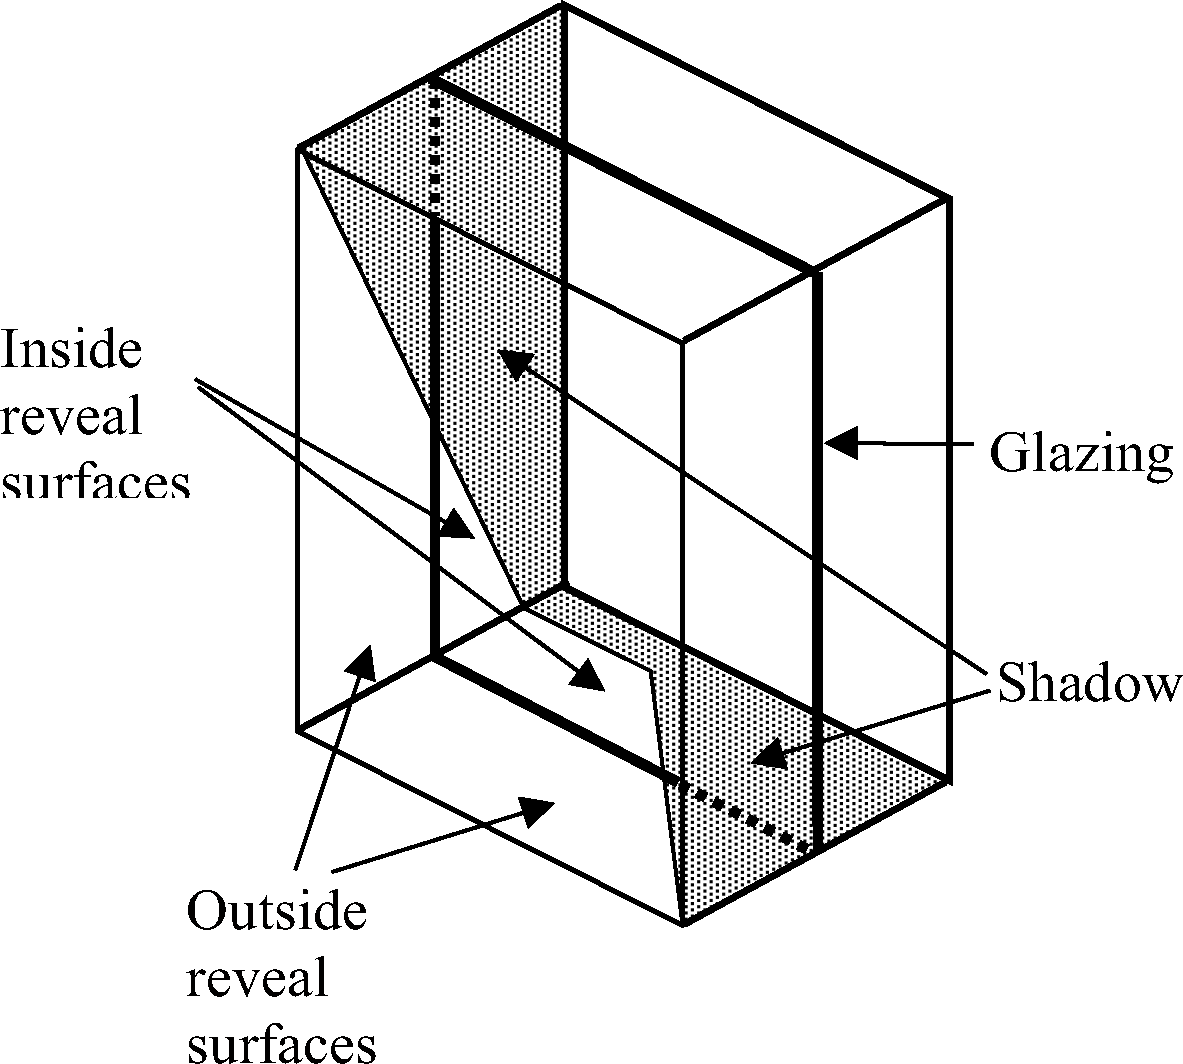
\includegraphics[width=0.9\textwidth, height=0.9\textheight, keepaspectratio=true]{media/image1593.png}
\caption{Example of shadowing of reveal surfaces by other reveal surfaces. \protect \label{fig:example-of-shadowing-of-reveal-surfaces-by}}
\end{figure}

The size of the shadowed areas, and the size of the corresponding illuminated areas, depends on the following factors:

\begin{itemize}
\item
  The sun position relative to the window
\item
  The height and width of the window
\item
  The depth of the outside and inside reveal surfaces
\end{itemize}

We will assume that the reveal surfaces are perpendicular to the window plane and that the window is rectangular. Then the above factors determine a unique shadow pattern. From the geometry of the pattern the shadowed areas and corresponding illuminated areas can be determined. This calculation is done in subroutine CalcBeamSolarReflectedFromWinRevealSurface in the SolarShading module. The window reveal input data is specified in the WindowProperty:FrameAndDivider object expect for the depth of the outside reveal, which is determined from the vertex locations of the window and its parent wall.

If an exterior shading device (shade, screen or blind) is in place it is assumed that it blocks beam solar before it reaches outside or inside reveal surfaces. Correspondingly, it is assumed that an interior or between-glass shading device blocks beam solar before it reaches inside reveal surfaces.

Representative shadow patterns are shown in Figures~\ref{fig:expression-for-area-of-shaded-regions-part-a} and~\ref{fig:expression-for-area-of-shaded-regions-part-b} for a window with no shading device, and without and with a frame. The case with a frame has to be considered separately because the frame can cast an additional shadow on the inside reveal surfaces.

The patterns shown apply to both vertical and horizontal reveal surfaces. It is important to keep in mind that, for a window of arbitrary tilt, if the left reveal surfaces are illuminated the right surfaces will not be, and vice versa. And if the bottom reveal surfaces are illuminated the top surfaces will not be, and vice versa. (Of course, for a vertical window, the top reveal surfaces will never be illuminated by beam solar if the reveal surfaces are perpendicular to the glazing, as is being assumed.

For each shadow pattern in Figures~\ref{fig:expression-for-area-of-shaded-regions-part-a} and~\ref{fig:expression-for-area-of-shaded-regions-part-b}, equations are given for the shadowed areas \({A_{1,sh}}\) ~and \emph{\({A_{2,sh}}\)}~of the outside and inside reveal surfaces, respectively. The variables in these equations are the following (see also Figure~\ref{fig:vertical-section-through-a-vertical-window}):

\({d_1}\) ~~~~~~~ = depth of outside reveal, measured from the outside plane of the glazing to the edge of the reveal, plus one half of the glazing thickness.

\({d_2}\) ~~ ~~~~~ = depth of inside reveal (or, for illumination on bottom reveal surfaces,~ inside sill depth), measured from the inside plane of the glazing to the edge of the reveal or the sill, plus one half of the glazing thickness.

\(L\) ~~~~~~~ = window height for vertical reveal surfaces or window width for horizontal reveal surfaces

\(\alpha\) ~~~~~~~~~ = vertical solar profile angle for shadowing on vertical reveal surfaces or horizontal solar profile angle for shadowing on horizontal reveal surfaces.

\({p_1}({p_2})\) ~ = distance from outside (inside) surface of frame to glazing midplane.

\({d_2}^\prime\) ~~~~~ = depth of shadow cast by top reveal on bottom reveal, or by left reveal on right reveal, or by right reveal on left reveal.

\({d_2}^{\prime \prime }\) ~~~~ = depth of shadow cast by frame.

For simplicity it is assumed that, for the case without a frame, the shadowed and illuminated areas extend into the glazing region. For this reason, \({d_1}\) and \({d_2}\) are measured from the midplane of the glazing. For the case with a frame, the beam solar absorbed by the surfaces formed by the frame outside and inside projections perpendicular to the glazing is calculated as described in ``Window Frame and Divider Calculation: Calculation of Solar Radiation Absorbed by Frame.''

\begin{figure}[htbp]
\centering
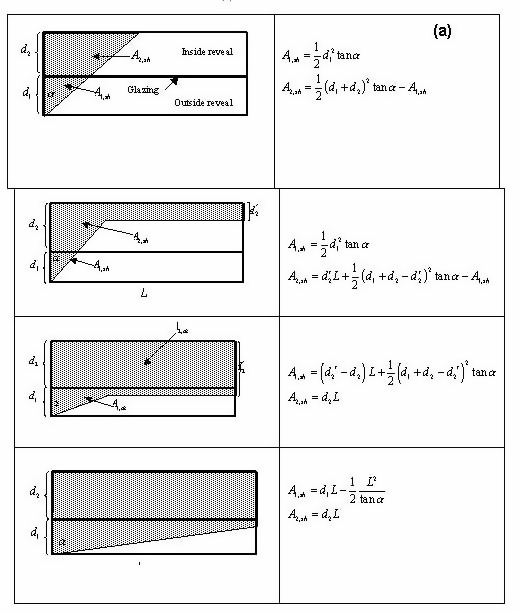
\includegraphics{media/image1605.png}
\caption{Expression for area of shaded regions for different shadow patterns: (a) window without frame}
\label{fig:expression-for-area-of-shaded-regions-part-a}
\end{figure}

\begin{figure}[htbp]
\centering
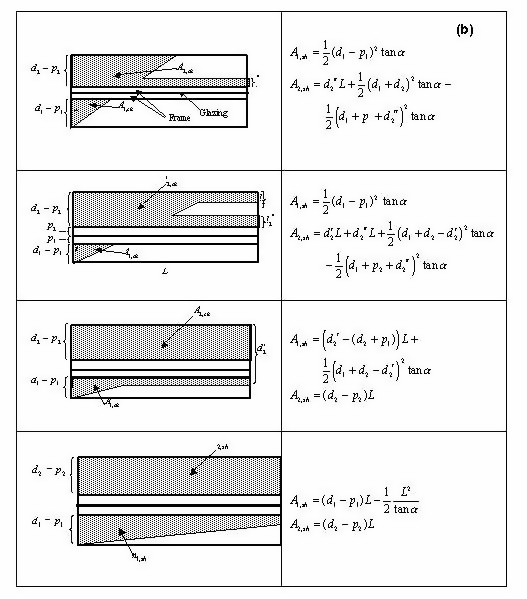
\includegraphics{media/image1606.png}
\caption{Expression for area of shaded regions for different shadow patterns: (b) window with frame}
\label{fig:expression-for-area-of-shaded-regions-part-b}
\end{figure}

\begin{figure}[hbtp] % fig 100
\centering
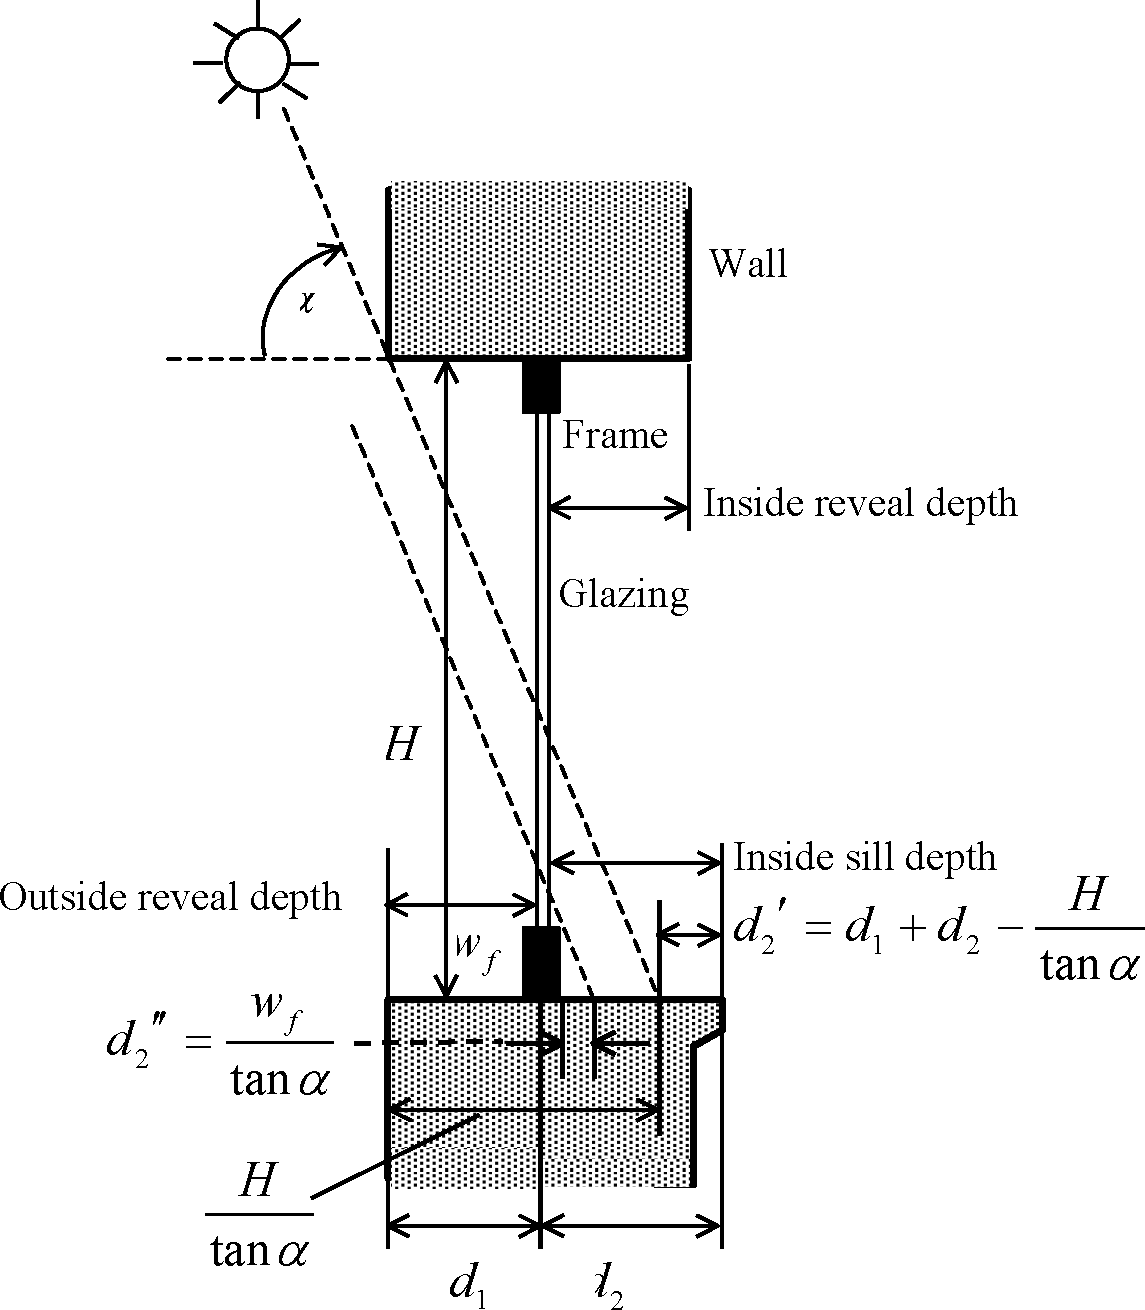
\includegraphics[width=0.9\textwidth, height=0.9\textheight, keepaspectratio=true]{media/image1607.png}
\caption{Vertical section through a vertical window with outside and inside reveal showing calculation of the shadows cast by the top reveal onto the inside sill and by the frame onto the inside sill. \protect \label{fig:vertical-section-through-a-vertical-window}}
\end{figure}

The following logic gives expressions for the shadowed areas for all possible shadow patterns. Here:

d1 = \({d_1}\)

d2 = \({d_2}\)

P1 = \({p_1}\)

P2 = \({p_2}\)

f1 = \({d_1} - {p_1}\)

f2 = \({d_2} - {p_2}\)

d2prime = \({d_2}^\prime\)

d2prime2 = \({d_2}^{\prime \prime }\)

d12 = \({d_1} + {d_2} - {d_2}^\prime\)

TanAlpha = \(\tan \alpha\)

A1sh = \({A_{1,sh}}\)

A2sh = \({A_{2,sh}}\)

L = \(L\)

L1 = average distance to frame of illuminated area of outside reveal (used to calculate view factor to frame).

L2 = average distance to frame of illuminated area of inside reveal (used to calculate view factor to frame).

\begin{lstlisting}
 IF(window does not have a frame) THEN
      IF(d2prime < = d2) THEN
     IF(d12*TanAlpha < = L) THEN
       A1sh = 0.5*TanAlpha*d1**2
       A2sh = d2prime*L + 0.5*TanAlpha*d12**2 - A1sh
     ELSE  ! d12*TanAlpha > L
       IF(d1*TanAlpha < = L) THEN
         A1sh = 0.5*TanAlpha*d1**2
         A2sh = d2*L - 0.5*TanAlpha*(L/TanAlpha - d1)**2
       ELSE  ! d1*TanAlpha > L
         A1sh = d1*L - (0.5/TanAlpha)*L**2
         A2sh = d2*L
       END IF
     END IF
   ELSE  ! d2prime > d2
     A2sh = d2*L
     IF(d2prime < d1+d2) THEN
       IF(d12*TanAlpha < = L) THEN
         A1sh = L*(d2prime-d2) + 0.5*TanAlpha*d12**2
       ELSE  ! d12*TanAlpha > L
         A1sh = d1*L - 0.5*L**2/TanAlpha
       END IF
     ELSE  ! d2prime > = d1+d2
       A1sh = d1*L
     END IF
   END IF
 ELSE  ! Window has a frame
  f1 = d1-P1
  f2 = d2-P2
  d2prime2 = FrameWidth/TanGamma
  IF(vertical reveal) THEN  ! Vertical reveal
    IF(InsReveal+0.5*GlazingThickness < = P2) d2 = P2 + 0.001
  ELSE                      ! Horizontal
    IF(bottom reveal surfaces may be illuminated) THEN
      ! Bottom reveal surfaces may be illuminated
      IF(InsSillDepth+0.5*GlazingThickness< = P2) d2 = P2 + 0.001
    ELSE
      ! Top reveal surfaces may be illuminated
      IF(InsReveal+0.5*GlazingThickness < = P2) d2 = P2 + 0.001
    END IF
  END IF
  IF(d2prime < = f2) THEN
    ! Shadow from opposing reveal does not go beyond inside
     !  surface of frame
    IF(d12*TanAlpha < = L) THEN
      A1sh = 0.5*TanAlpha*f1**2
      L1   = f1*(f1*TanAlpha/(6*L)+0.5)
      IF(d2-(d2prime+d2prime2+P2) > = 0.) THEN
        A2sh = (d2prime+d2prime2)*L + &
          0.5*TanAlpha*((d1+d2-d2prime)**2-d1+p2+d2prime2)**2)
        L2   = d2prime2 + 0.5*(d2-(d2prime+d2prime2+P2))
      ELSE  ! d2-(d2prime+d2prime2+P2) < 0.
        ! Inside reveal is fully shadowed by frame and/or
         !opposing reveal
        A2sh = f2*L
        L2   = f2
      END IF
    ELSE  ! d12*TanAlpha > = L
      IF((d1+P2)*TanAlpha < = L) THEN
        A1sh = 0.5*TanAlpha*f1**2
        L1 = f1*((f1*TanAlpha)/(6*L) + 0.5)
        IF((d1+P2+d2prime2)*TanAlpha > = L) THEN
          A2sh = f2*L
          L2   = f2
        ELSE  ! (d1+P2+d2prime2)*TanAlpha < L
          A2sh = f2*L - 0.5*(L-(d1+P2)*TanAlpha)**2/TanAlpha &
             + d2prime2*(L-(d1+P2+d2prime2/2)*TanAlpha)
          L2 = d2prime2 + (L/TanAlpha - (d1+P2+d2prime2))/3
        END IF
      ELSE  ! (d1+P2)*TanAlpha > L
        L2 = f2
        A2sh = f2*L
        IF(f1*TanAlpha < = L) THEN
          A1sh = 0.5*TanAlpha*f1**2
          L1 = f1*((f1*TanAlpha)/(6*L) + 0.5)
        ELSE  ! f1*TanAlpha > L
          A1sh = f1*L - 0.5*L**2/TanAlpha
          L1 = f1-(L/TanAlpha)/3
        END IF
      END IF
    END IF
  ELSE
     ! d2prime > f2 -- Shadow from opposing reveal goes beyond
     ! inside of frame
    A2sh = f2*L
    L2 = f2
    IF(d2prime > = d1+d2) THEN
      A1sh = 0.0
      L1   = f1
    ELSE  ! d2prime < d1+d2
      IF(d2prime < = d2+P1) THEN
        IF(f1*TanAlpha < = L) THEN
          A1sh = 0.5*TanAlpha*f1**2
          L1 = f1*((f1*TanAlpha)/(6*L) + 0.5)
        ELSE  ! f1*TanAlpha > L
          A1sh = f1*L - 0.5*L**2/TanAlpha
              L1   = f1 - (L/TanAlpha)/3
            END IF
          ELSE  ! d2prime > d2+P1
            IF(d12*TanAlpha < = L) THEN
              A1sh = L*(d2prime-(d2+P1)) + 0.5*TanAlpha*d12**2
              L1   = (L*(f1-d12/2)-d12*TanAlpha* &
                 (f1/2-d12/3))/(L-d12*TanAlpha/2)
            ELSE  ! d12*TanAlpha > L
              A1sh = f1*L - 0.5*L**2/TanAlpha
              L1   = f1 - (L/TanAlpha)/3
            END IF
          END IF
        END IF
      END IF
      FracToGlassOuts = 0.5*(1.0 - ATAN(FrameWidth/L1)/PiOvr2)
      FracToGlassIns  = 0.5*(1.0 - ATAN(FrameWidth/L2)/PiOvr2)
    END IF  ! End of check if window has frame
\end{lstlisting}

The beam solar reflected from a sunlit region of area \(A\) is given by:

\begin{equation}
R = {I_B}A\cos \beta (1 - a){\rm{ }}
\end{equation}

where

\(R\) = reflected solar radiation {[}W{]}

\({I_B}\) = beam normal irradiance {[}W/m\(^{2}\){]}

\(A\) = sunlit area {[}m\(^{2}\){]}

\(\beta\) = beam solar angle of incidence on reveal surface

\(a\) = solar absorptance of reveal surface

All reflected radiation is assumed to be isotropic diffuse. For outside reveal surfaces it is assumed that \(R/2\) ~goes toward the window and \(R/2\) ~goes to the exterior environment. Of the portion that goes toward the window a fraction \({F_1}\) ~goes toward the frame, if present, and \(1 - {F_1}\) ~goes toward the glazing.

The view factor \({F_1}\) to the frame calculated by assuming that the illuminated area can be considered to be a line source. Then the area-weighted average distance, \({L_1}\), of the source to the frame is calculated from the shape of the illuminated area (see above psuedo-code). Then \({F_1}\) is related as follows to the average angle subtended by the frame of width \({w_f}\):

\begin{equation}
{F_1} = \frac{{{{\tan }^{ - 1}}({w_f}/{L_1})}}{{\pi /2}}
\end{equation}

For the portion going towards the frame, \((R/2){F_1}{a_f}\) is absorbed by the frame (where \({a_f}\) is the solar absorptance of the frame) and contributes to the frame heat conduction calculation. The rest, \((R/2){F_1}(1 - {a_f})\) , is assumed to be reflected to the exterior environment.

If the glazing has diffuse transmittance \({\tau_{diff}}\), diffuse front reflectance \(\rho_{diff}^f\), and layer front absorptance \(\alpha_{l,diff}^f\), then, of the portion, \((R/2)(1 - {F_1})\), that goes toward the glazing, \((R/2)(1 - {F_1}){\tau_{diff}}\) is transmitted to the zone, \((R/2)(1 - {F_1})\alpha_{l,diff}^f\) is absorbed in glass layer \(l\) and contributes to the glazing heat balance calculation, and \((R/2)(1 - {F_1})\rho_{dif{f_{}}}^f\) is reflected to the exterior environment.

The beam solar absorbed by an outside reveal surface is added to the other solar radiation absorbed by the outside of the window's parent wall.

For inside reveal surfaces it is assumed that \(R/2\) ~goes towards the window and \(R/2\) ~goes into the zone. Of the portion that goes toward the window a fraction \((R/2){F_2}\) ~goes toward the frame, if present, and \((R/2)(1 - {F_2})\) goes toward the glazing (\({F_2}\)~is calculated using a method analogous to that used for \({F_1}\)). For the portion going towards the frame, \((R/2){F_2}{a_f}\) is absorbed by the frame and contributes to the frame heat conduction calculation. The rest, \((R/2){F_2}(1 - {a_f})\), is assumed to be reflected back into the zone.

If the glazing has diffuse back reflectance \(\rho_{diff}^b\), and layer back absorptance \(\alpha_{l,diff}^b\), then, of the portion \((R/2)(1 - {F_2})\)~that goes toward the glazing, \((R/2)(1 - {F_2}){\tau_{diff}}\) is transmitted back out the glazing, \((R/2)(1 - {F_2})\alpha_{l,diff}^b\) is absorbed in glass layer \(l\) and contributes to the glazing heat balance calculation, and \((R/2)(1 - {F_2})\rho_{dif{f_{}}}^b\) is reflected into the zone.

The beam solar absorbed by an inside reveal surface is added to the other solar radiation absorbed by the inside of the window's parent wall.

\subsection{Shading Device Thermal Model}\label{shading-device-thermal-model}

Shading devices in EnergyPlus can be on the exterior or interior sides of the window or between glass layers. The window shading device thermal model accounts for the thermal interactions between the shading layer (shade, screen or blind) and the adjacent glass, and between the shading layer and the room (for interior shading) or the shading layer and the outside surround (for exterior shading).

An important feature of the shading device thermal model is calculating the natural convection airflow between the shading device and glass. This flow affects the temperature of the shading device and glazing and, for interior shading, is a determinant of the convective heat gain from the shading layer and glazing to the zone air. The airflow model is based on one described in the ISO Standard 15099, ``Thermal Performance of Windows, Doors and Shading Devices---Detailed Calculations'' {[}ISO15099, 2001{]}. (Between-glass forced airflow is also modeled; see ``Airflow Windows.'')

The following effects are considered by the shading device thermal model:

\begin{itemize}
\item
  For interior and exterior shading device: Long-wave radiation (IR) from the surround absorbed by shading device, or transmitted by the shading device and absorbed by the adjacent glass. For interior shading the surround consists of the other zone surfaces. For exterior shading the surround is the sky and ground plus exterior shadowing surfaces and exterior building surfaces ``seen'' by the window.
\item
  Inter-reflection of IR between the shading device and adjacent glass.
\item
  Direct and diffuse solar radiation absorbed by the shading device.
\item
  Inter-reflection of solar radiation between shading layer and glass layers.
\item
  Convection from shading layer and glass to the air in the gap (or, for between-glass shading, gaps) between the shading layer and adjacent glass, and convection from interior shading layer to zone air or from exterior shading layer to outside air.
\item
  Natural convection airflow in the gap (or, for between-glass shading, gaps) between shading layer and adjacent glass induced by buoyancy effects, and the effect of this flow on the shading-to-gap and glass-to-gap convection coefficients.
\item
  For interior shading, convective gain (or loss) to zone air from gap airflow.
\end{itemize}

In the following it is assumed that the shading device, when in place, covers the glazed part of the window (and dividers, if present) and is parallel to the glazing. For interior and exterior shading devices it is assumed that the shading layer is separated from the glazing by an air gap. A between-glass shading layer is assumed to be centered between two glass layers and separated from the adjacent glass layers by gaps that is filled with the same gas. If the window has a frame, it is assumed that the shading device does \emph{not} cover the frame.

\subsection{Heat Balance Equations for Shading Device and Adjacent Glass}\label{heat-balance-equations-for-shading-device-and-adjacent-glass}

If a window shading device is deployed the heat balance equations for the glass surfaces facing the shading layer are modified, and two new equations, one for each face of the shading layer, are added. Figure~\ref{fig:glazing-system-with-two-glass-layers-and-an} illustrates the case of double glazing with an interior shading device.

\begin{figure}[hbtp] % fig 101
\centering
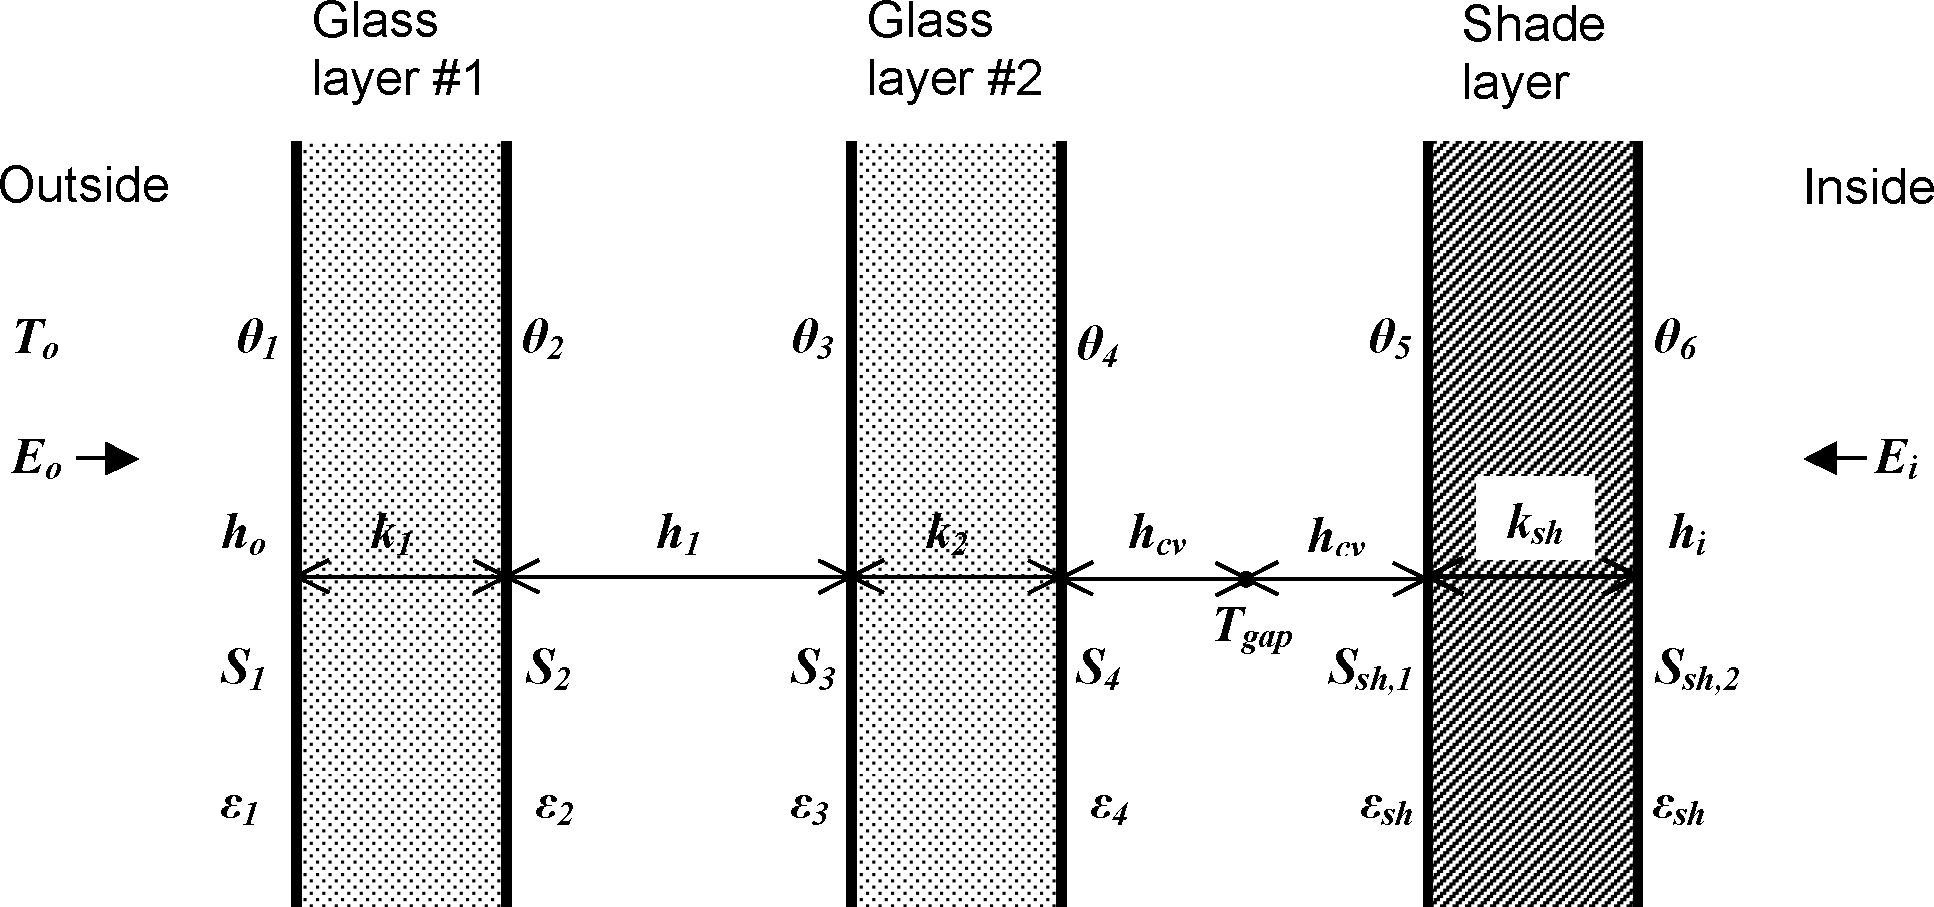
\includegraphics[width=0.9\textwidth, height=0.9\textheight, keepaspectratio=true]{media/image1663.png}
\caption{Glazing system with two glass layers and an interior shading layer showing variables used in heat balance equations. \protect \label{fig:glazing-system-with-two-glass-layers-and-an}}
\end{figure}

The heat balance equation for the glass surface facing the gap between glass and shading layer (called in the following, ``gap'') is:

\begin{equation}
\frac{{{E_i}{\varepsilon_4}{\tau_{sh}}}}{{1 - {\rho_4}{\rho_{sh}}}} + \frac{{\sigma {\varepsilon_4}}}{{1 - {\rho_4}{\rho_{sh}}}}\left[ {\theta_5^4{\varepsilon_{sh}} - \theta_4^4(1 - {\rho_{sh}})} \right] + {k_2}\left( {{\theta_3} - {\theta_4}} \right) + {h_{cv}}\left( {{T_{gap}} - {\theta_4}} \right) + {S_4} = 0
\end{equation}

where

\emph{$\tau$\(_{sh}\)} = IR diffuse transmittance of shading device

\emph{$\varepsilon$\(_{sh}\)} = diffuse emissivity of shading device

\emph{$\rho$\(_{sh}\)} = IR diffuse reflectance of shading device ( = 1 - ( \emph{$\tau$\(_{sh}\)} + \emph{$\varepsilon$\(_{sh}\)}))

\emph{$\theta$\(_{5}\)} = temperature of the surface of the shading layer that faces the gap (K).

The term 1 - \emph{$\rho$\(_{4}\)$\rho$\(_{sh}\)} accounts for the inter-reflection of IR radiation between glass and shading layer.

The convective heat transfer from glass layer \#2 to the air in the gap is:

\begin{equation}
{q_{c,gl}} = {h_{cv}}({\theta_4} - {T_{gap}})
\end{equation}

where

\emph{T\(_{gap}\)} = effective mean temperature of the gap air (K).

\emph{h\(_{cv}\)} = convective heat transfer coefficient from glass or shading layer to gap air (W/m\(^{2}\)K).

The corresponding heat transfer from shading layer to gap air is:

\begin{equation}
{q_{c,sh}} = {h_{cv}}({\theta_5} - {T_{gap}})
\end{equation}

The convective heat transfer coefficient is given by:

\begin{equation}
{h_{cv}} = 2{h_c} + 4v
\label{eq:hcvConvectiveCoefficientEquation}
\end{equation}

where

\emph{h\(_{c}\)} = surface-to-surface heat transfer coefficient for non-vented (closed) cavities (W/m\(^{2}\)K)

\emph{v} = mean air velocity in the gap (m/s).

The quantities \emph{h\(_{cv}\)} and \emph{T\(_{gap}\)} depend on the airflow velocity in the gap, which in turn depends on several factors, including height of shading layer, glass/shading layer separation (gap depth), zone air temperature for interior shading or outside air temperature for exterior shading, and shading layer and glass face temperatures. The calculation of \emph{h\(_{cv}\)} and \emph{T\(_{gap}\)} is described in the following sections.

The heat balance equation for the shading layer surface facing the gap is:

\begin{equation}
\frac{E_i \tau_{sh} \rho_4 \varepsilon_{sh}} {1 - \rho_4 \rho_{sh}} + 
  \frac{\sigma \varepsilon_{sh}} {1 - \rho_4 \rho_{sh}} \left[
    \varepsilon_4 \theta_4^4 - \theta_5^4 (
      1 - \rho_4( 
        \varepsilon_{sh} + \rho_{sh}
      )
    )
  \right] + 
  k_{sh} \left(
    \theta_6 - \theta_5
  \right) + 
  h_{cv} \left(
    T_{gap} - \theta_5
  \right) + 
  S_{sh,1} = 0
\end{equation}

where

\emph{k\(_{sh}\)} = shading layer conductance (W/m\(^{2}\)K).

\emph{$\theta$\(_{6}\)} = temperature of shading layer surface facing the zone air (K).

\emph{S\(_{sh,l}\)} = solar radiation plus short-wave radiation from lights plus IR radiation from lights and zone equipment absorbed by the gap-side face of the shading layer (W/m\(^{2}\)K).

The heat balance equation for the shading layer surface facing the zone air is:

\begin{equation}
{E_i}{\varepsilon_{sh}} - {\varepsilon_{sh}}\sigma \theta_6^4 + {k_{sh}}\left( {{\theta_5} - {\theta_6}} \right) + {h_i}\left( {{T_i} - {\theta_6}} \right) + {S_{sh,2}} = 0
\end{equation}

where

\emph{S\(_{sh,2}\)} = solar radiation plus short-wave radiation from lights plus IR radiation from lights and zone equipment absorbed by the zone-side face of the shading layer (W/m\(^{2}\)K).

\subsection{Solving for Gap Airflow and Temperature}\label{solving-for-gap-airflow-and-temperature}

For interior and exterior shading devices a pressure-balance equation is used to determine gap air velocity, gap air mean equivalent temperature and gap outlet air temperature given values of zone air temperature (or outside temperature for exterior shading), shading layer face temperatures and gap geometry. The pressure balance equates the buoyancy pressure acting on the gap air to the pressure losses associated with gap airflow between gap inlet and outlet {[}ISO15099, 2001{]}. The variables used in the following analysis of the interior shading case are shown in Figure~\ref{fig:vertical-section-a-and-perspective-view-b-of}.

\begin{figure}[hbtp] % fig 102
\centering
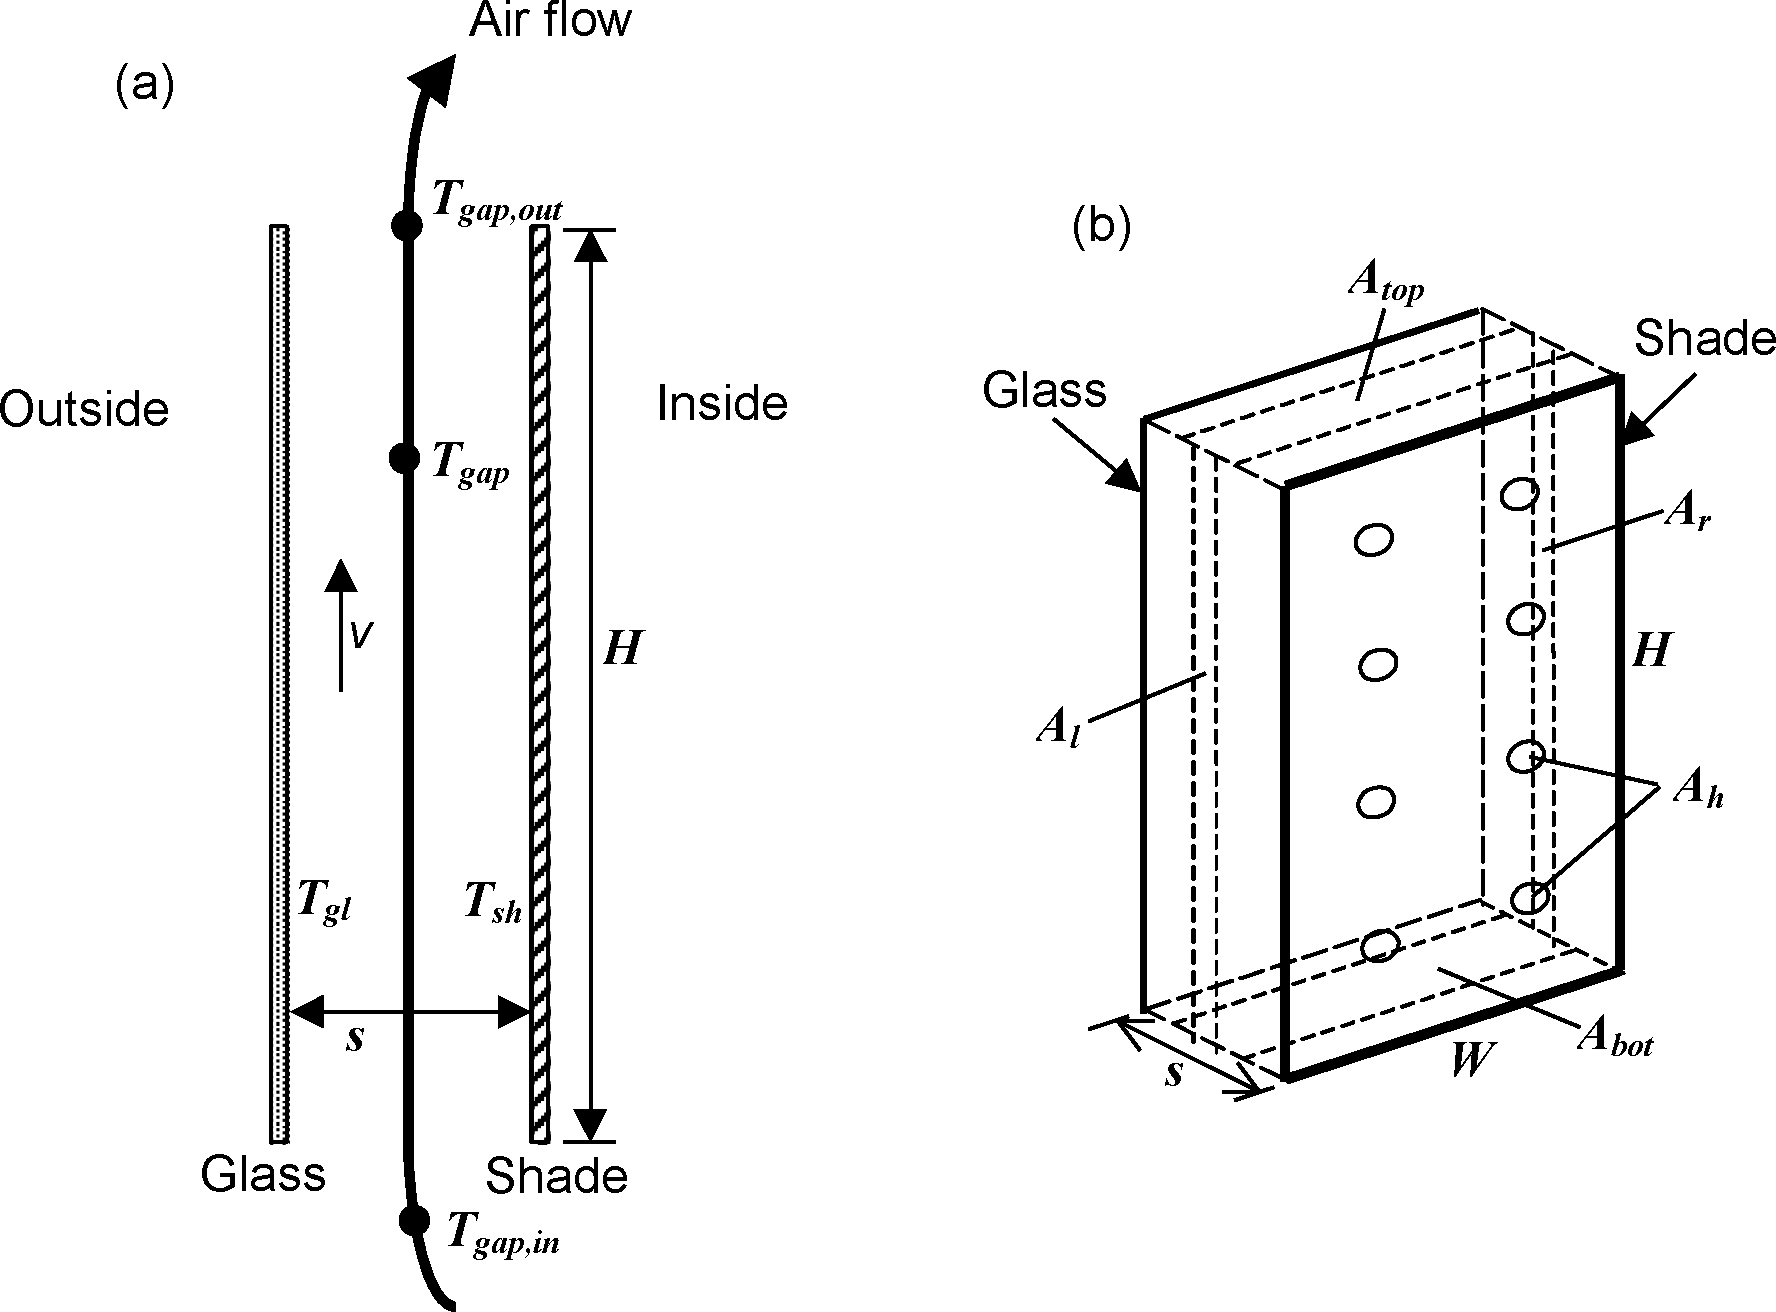
\includegraphics[width=0.9\textwidth, height=0.9\textheight, keepaspectratio=true]{media/image1670.png}
\caption{Vertical section (a) and perspective view (b) of glass layer and interior shading layer showing variables used in the gap airflow analysis. The opening areas A\(_{bot}\), A\(_{top}\), A\(_{l}\), A\(_{r}\) and A\(_{h}\) are shown schematically. \protect \label{fig:vertical-section-a-and-perspective-view-b-of}}
\end{figure}

\subsubsection{Pressure Balance Equation}\label{pressure-balance-equation}

The pressure balance equation for airflow through the gap is:

\begin{equation}
\Delta {p_T} = \Delta {p_B} + \Delta {p_{HP}} + \Delta {p_Z}
\label{eq:PressureBalanceEquationAirflow}
\end{equation}

Here, \emph{Δp\(_{T}\)} is the driving pressure difference between room air and gap air. It is given by:

\begin{equation}
\Delta {p_T} = {\rho_0}{T_0}gH\sin \phi \frac{{\left| {{T_{gap}} - {T_{gap,in}}} \right|}}{{{T_{gap}}{T_{gap,in}}}}
\end{equation}

where

\emph{$\rho$\(_{0}\)} = density of air at temperature \emph{T\(_{0}\)} (kg/m\(^{3}\))

\emph{T\(_{0}\)} = reference temperature (283K)

\emph{g} = acceleration due to gravity (m/s\(^{2}\))

\emph{H} = height of shading layer (m)

\emph{$\phi$} = tilt angle of window (vertical = 90\(^{o}\))

\emph{T\(_{gap}\)} = effective mean temperature of the gap air (K)

\emph{T\(_{gap,in}\)} = gap inlet temperature ( = zone air temperature for interior shading) (K)

The \emph{Δp\(_{B}\)} term is due to the acceleration of air to velocity \emph{v} (Bernoulli's law). It is given by:

\begin{equation}
\Delta {p_B} = \frac{\rho }{2}{v^2}{\rm{    (Pa)}}
\end{equation}

where \emph{$\rho$}~is the gap air density evaluated at \emph{T\(_{gap}\)} (kg/m\(^{3}\)).

The \emph{Δp\(_{HP}\)} term represents the pressure drop due to friction with the shading layer and glass surfaces as the air moves through the gap. Assuming steady laminar flow, it is given by the Hagen-Poiseuille law for flow between parallel plates {[}Munson et al. 1998{]}:

\begin{equation}
\Delta {p_{HP}} = 12\mu \frac{H}{{{s^2}}}{v^{}}{\rm{    (Pa)}}
\end{equation}

where \emph{$\mu$} is the viscosity of air at temperature \emph{T\(_{gap}\)} (Pa-s).

The \emph{Δp\(_{Z}\)} term is the sum of the pressure drops at the inlet and outlet openings:

\begin{equation}
\Delta {p_Z} = \frac{{\rho {v^2}}}{2}\left( {{Z_{in}} + {Z_{out}}} \right){\rm{    (Pa)}}
\end{equation}

Here, the inlet pressure drop factor, Z\(_{in}\), and the outlet pressure drop factor, Z\(_{out}\), are given by:

\begin{equation}
  \begin{array}{rl}
    Z_{in}  & = \left( \frac{A_{gap}}{0.66A_{eq,in}}  - 1 \right)^2 \\
    Z_{out} & = \left( \frac{A_{gap}}{0.60A_{eq,out}} - 1 \right)^2
  \end{array}
\end{equation}

where

\emph{A\(_{eq,in}\)} = equivalent inlet opening area (m\(^{2}\))

\emph{A\(_{eq,out}\)} = equivalent outlet opening area (m\(^{2}\))

\emph{A\(_{gap}\)} = cross-sectional area of the gap = \emph{sW}(m\(^{2}\))

If T\(_{gap}\) \textgreater{} T\(_{gap,in}\):

\begin{equation}
  \begin{array}{rl}
    A_{eq,in}  & = A_{bot} + \frac{A_{top}}{2(A_{bot}+A_{top}} \left( A_l + A_r + A_h \right) \\
    A_{eq,out} & = A_{top} + \frac{A_{bot}}{2(A_{bot}+A_{top}} \left( A_l + A_r + A_h \right) 
  \end{array}
\end{equation}

If T\(_{gap}\) \(\leq\) T\(_{gap,in}\):

\begin{equation}
  \begin{array}{rl}
    A_{eq,in}  & = A_{top} + \frac{A_{bot}}{2(A_{bot}+A_{top}} \left( A_l + A_r + A_h \right) \\
    A_{eq,out} & = A_{bot} + \frac{A_{top}}{2(A_{bot}+A_{top}} \left( A_l + A_r + A_h \right) 
  \end{array}
\end{equation}

Here, the area of the openings through which airflow occurs (see Figure~\ref{fig:vertical-section-a-and-perspective-view-b-of} and Figure~\ref{fig:examples-of-openings-for-an-interior-shading}) are defined as follows:

A\(_{bot}\) = area of the bottom opening (m\(^{2}\))

A\(_{top}\) = area of the top opening (m\(^{2}\))

A\(_{l}\) = area of the left-side opening (m\(^{2}\))

A\(_{r}\) = area of the right-side opening (m\(^{2}\))

A\(_{h}\) = air permeability of the shading device expressed as the total area of openings (``holes'') in the shade surface (these openings are assumed to be uniformly distributed over the shade) (m\(^{2}\))

Figure~\ref{fig:examples-of-openings-for-an-interior-shading} shows examples of A\(_{bot}\), A\(_{top}\), A\(_{l}\) and A\(_{r}\) for different shading device configurations.~ These areas range from zero to a maximum value equal to the associated shade/screen/blind-to-glass cross-sectional area; i.e., A\(_{bot}\) and A\(_{top}\) ≤ sW,~ A\(_{l}\) and A\(_{r}\) ≤ sH.

\begin{figure}[hbtp] % fig 103
\centering
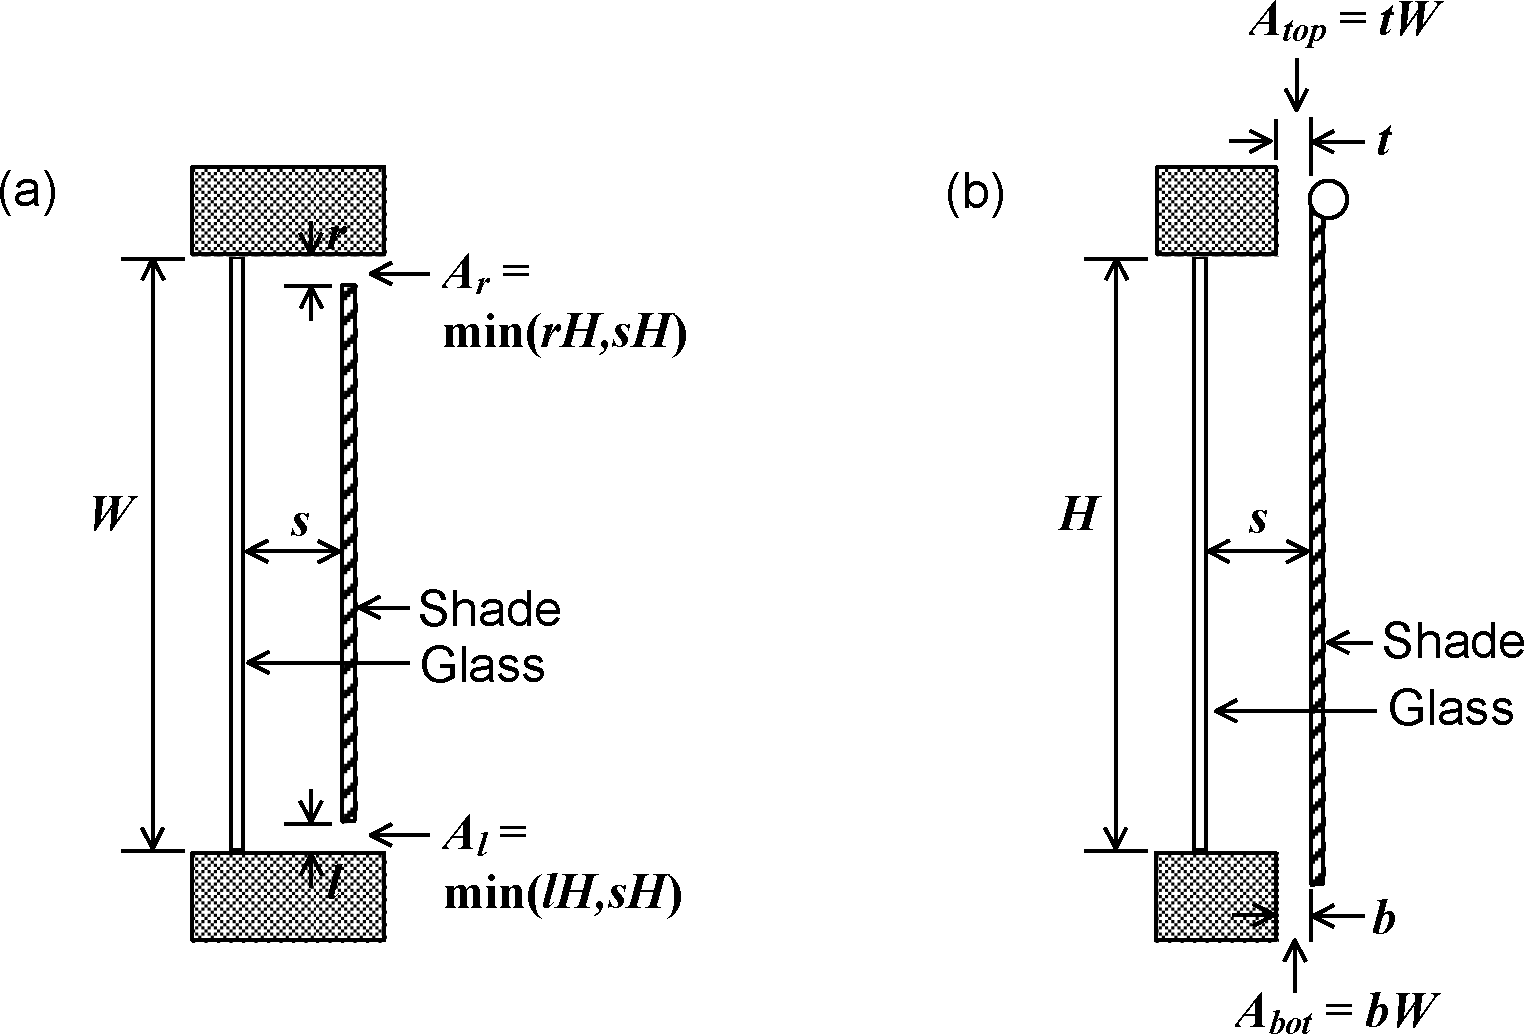
\includegraphics[width=0.9\textwidth, height=0.9\textheight, keepaspectratio=true]{media/image1679.png}
\caption{Examples of openings for an interior shading layer covering glass of height H and width W. Not to scale. (a) Horizontal section through shading layer with openings on the left and right sides (top view). (b) Vertical section through shading layer with openings at the top and bottom (side view). \protect \label{fig:examples-of-openings-for-an-interior-shading}}
\end{figure}

Expression for the Gap Air Velocity

Expressing Equation~\ref{eq:PressureBalanceEquationAirflow} in terms of~\emph{v}~yields the following quadratic equation:

\begin{equation}
\frac{{\rho {v^2}}}{2}\left( {1 + {Z_{in}} + {Z_{out}}} \right) + \frac{{12\mu H}}{{{s^2}}}v - {\rho_0}{T_0}gH\sin \phi \frac{{\left| {{T_{gap,in}} - {T_{gap}}} \right|}}{{{T_{gap,in}}{T_{gap}}}} = 0
\end{equation}

Solving this gives:

\begin{equation}
v = \frac{{{{\left[ {{{\left( {\frac{{12\mu H}}{{{s^2}}}} \right)}^2} + \frac{{2{\rho ^2}(1 + {Z_{in}} + {Z_{out}}){\rho_0}{T_0}gH\sin \phi \left| {{T_{gap,in}} - {T_{gap}}} \right|}}{{{T_{gap,in}}{T_{gap}}}}} \right]}^{1/2}} - \frac{{12\mu H}}{{{s^2}}}}}{{\rho (1 + {Z_{in}} + {Z_{out}})}}
\label{eq:GapAirVelocityEquation}
\end{equation}

The choice of the root of the quadratic equation is dictated by the requirement that \emph{v} = 0 if \emph{T\(_{gap,in}\)} = \emph{T\(_{gap}\)}.

Gap Outlet Temperature and Equivalent Mean Air Temperature

The temperature of air in the gap as a function of distance, \emph{h}, from the gap inlet (Figure~\ref{fig:variation-of-gap-air-temperature-with}) is:

\begin{equation}
{T_{gap}}(h) = {T_{ave}} - ({T_{ave}} - {T_{gap,in}}){e^{ - h/{H_0}}}
\end{equation}

where

\begin{equation}
{T_{ave}} = \frac{{{T_{gl}} + {T_{sh}}}}{2}
\label{eq:GlassShadingLayerAverageTemperature}
\end{equation}

is the average temperature of the glass and shading layer surfaces facing the gap (K).

\emph{H\(_{0}\)} = characteristic height (m), given by:

\begin{equation}
{H_0} = \frac{{\rho {C_p}s}}{{2{h_{cv}}}}v
\end{equation}

where \emph{C\(_{p}\)} is the heat capacity of air.

The gap outlet temperature is given by:

\begin{equation}
{T_{gap,out}} = {T_{ave}} - ({T_{ave}} - {T_{gap,in}}){e^{ - H/{H_0}}}
\label{eq:TgapoutEquation}
\end{equation}

The thermal equivalent mean temperature of the gap air is:

\begin{equation}
{T_{gap}} = \frac{1}{H}\int\limits_0^H {{T_{gap}}(h)dh = {T_{ave}} - \frac{{{H_0}}}{H}} \left( {{T_{gap,out}} - {T_{gap,in}}} \right)
\label{eq:TgapEquation}
\end{equation}

\begin{figure}[hbtp] % fig 104
\centering
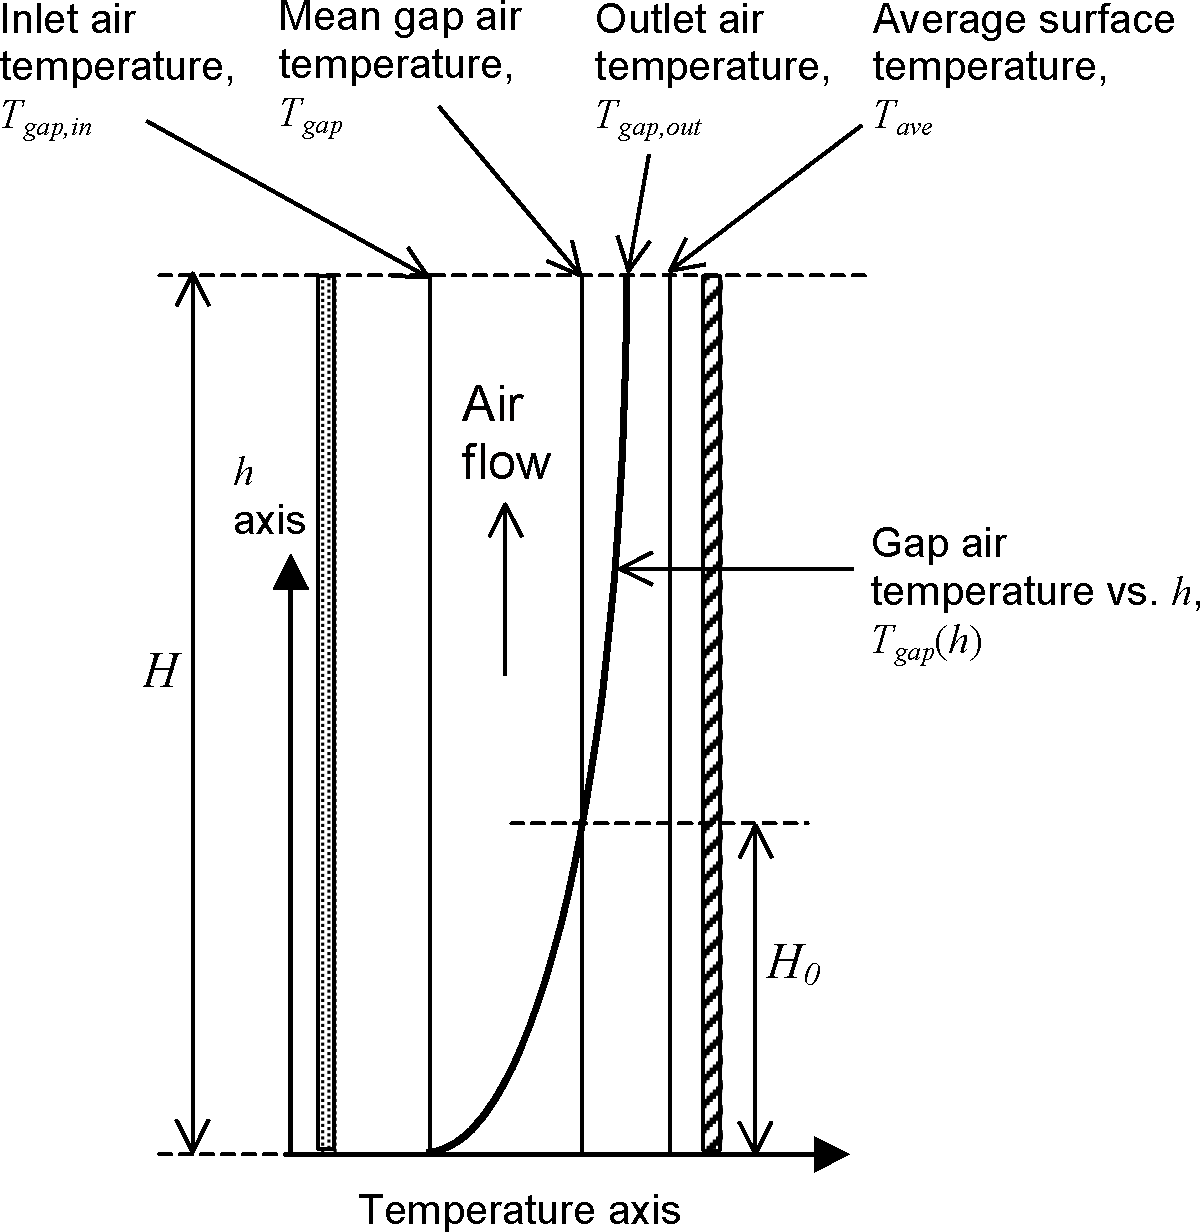
\includegraphics[width=0.9\textwidth, height=0.9\textheight, keepaspectratio=true]{media/image1687.png}
\caption{Variation of gap air temperature with distance from the inlet for upward flow. \protect \label{fig:variation-of-gap-air-temperature-with}}
\end{figure}

Solution Sequence for Gap Air Velocity and Outlet Temperature

The routine WinShadeGapFlow is called within the glazing heat balance iterative loop in SolveForWindowTemperatures to determine \emph{v} and \emph{T\(_{gap,out}\)}. The solution sequence in WinShadeGapFlow is as follows:

At start of iteration, guess \emph{T\(_{gap}\)} as ((\emph{T\(_{gl}\)} + \emph{T\(_{sh}\)})/2 + \emph{T\(_{gap,in}\)})/2. Thereafter use value from previous iteration.

Get still-air conductance, \emph{h\(_{c}\)}, by calling WindowGasConductance and NusseltNumber.

Get \emph{v} from Equation~\ref{eq:GapAirVelocityEquation}.

Get \emph{h\(_{cv}\)} from Equation~\ref{eq:hcvConvectiveCoefficientEquation}.

Get \emph{T\(_{ave}\)}from Equation~\ref{eq:GlassShadingLayerAverageTemperature}.

Get \emph{T\(_{gap,out}\)} from Equation~\ref{eq:TgapoutEquation}.

Get new value of \emph{T\(_{gap}\)}from Equation~\ref{eq:TgapEquation}.

The values of \emph{h\(_{cv}\)} and \emph{T\(_{gap}\)} so determined are then used in the window heat balance equations to find new values of the face temperatures of the glass and shading layers. These temperatures are used in turn to get new values of \emph{h\(_{cv}\)} and \emph{T\(_{gap}\)} until the whole iterative process converges.

Convective Heat Gain to Zone from Gap Airflow

The heat added (or removed) from the air as it passes through the gap produces a convective gain (or loss) to the zone air given by:

\begin{equation}
{q_v} = LW\left[ {{h_{cv}}\left( {{T_{gl}} - {T_{gap}}} \right) + {h_{cv}}\left( {{T_{sh}} - {T_{gap}}} \right)} \right] = 2{h_{cv}}LW\left( {{T_{ave}} - {T_{gap}}} \right){\rm{    (W)}}
\end{equation}

This can also be expressed as:

\begin{equation}
{q_v} = \dot m{C_p}\left( {{T_{gap,out}} - {T_{gap,in}}} \right){\rm{    (W)}}
\end{equation}

where the air mass flow rate in the gap is given by:

\begin{equation}
\dot m = \rho {A_{gap}}v{\rm{    (kg/s)}}
\end{equation}

\subsection{Improved Airflow Equations for Window Screens and Horizontal Louvered Blind Systems}
Several different approaches to simulate windows with attachments have been studied and developed. The primary focus of these works has been the experimental measurement, simulation, and simplified model development of solar heat gain for horizontal louvered blinds (venetian blinds) located between-glass and room-side. Relatively little research has been done to characterize the night-time (zero solar load) U-factor impacts of attachment products other than venetian blinds, including in-plane products such as solar screens, roller shades, cellular shades, insect screens, and drapes.

\begin{figure}[hbtp]
	\centering
	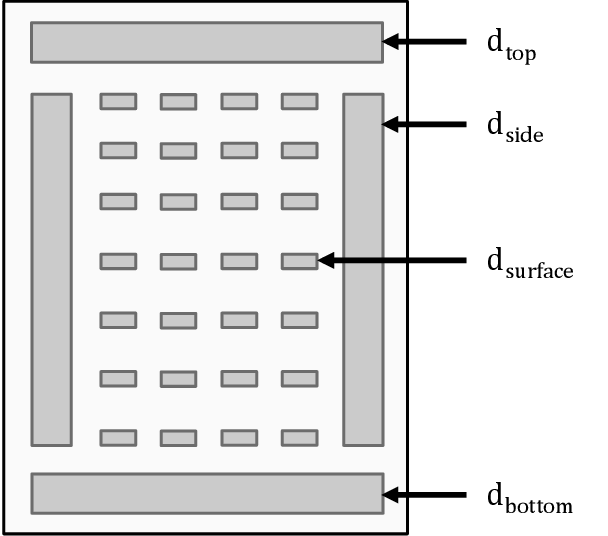
\includegraphics[width=0.9\textwidth, height=0.9\textheight, keepaspectratio=true]{media/WindowLayerAirflowOpennings.png}
	\caption{Illustration of ISO 15099 ventilated shade layer opening locations. \protect \label{fig:Openness_ISO15099}}
\end{figure}

Surface openness of shade systems, $d_{surface}$ in Figure~\ref{fig:Openness_ISO15099}, has primarily been studied for highly porous surfaces such as insect screens.
The inlet and outlet pressure loss of a cavity open to the indoor room, $\Delta P_z$, is calculated with Equations~\ref{eq:OpennesCalcs}, where the use of in/out and top/bot are dependent on the direction of flow, as determined by the glass surface temperature relative to the indoor temperature.

\begin{equation}
\begin{array}{rl}
\Delta P_{z}  & = 0.5 \rho v^2(Z_{in}+Z_{out}) \\
Z_{in/out} & = (\frac{A_s}{0.6A_{eq,in/out}}-1)^2 \\
A_{eq,in/out} & = A_{top/bot} + \frac{1}{2} \frac{A_{bot/top}}{A_{bot} + A_{top}}(A_l + A_r + A_h) \\
A_h & = d_{surface}WH \\
A_s & = d_{gap}W
\end{array}
\label{eq:OpennesCalcs}
\end{equation}

Where $\rho$ is the fluid density, $v$ s the fluid velocity, $Z_{in/out}$ is the pressure loss factor of the cavity, As is the cross-section area of the cavity, $d_{gap}$ is the glass-to-shade cavity depth, $d_{surface}$ is the openness fraction (0 - 1), W is the window width, H is the window height, $A_{eq}$, is the equivalent inlet/outlet area of the cavity, and Al, Ar, Atop, Abot, Ah are the areas of the left, right, top, bottom, and front surface ventilation gaps respectively. 

The set of equations~\ref{eq:OpennesCalcs} include an inherent minimum of pressure loss coefficient, Z, when the calculated inlet or outlet area, $A_{eq}$, equals 5/3 the cross section area, As. This limits the validity of the model to $A_{eq}$ less than 5/3 of As. Figure~\ref{fig:PressureLossFacor} illustrates this minimum with a surface map of calculated Z values (log(Z) plotted to show contours) over a range of $A_{eq}$ based on a 1m x 1m window. Figure~\ref{fig:PressureLossFacor} shows a slice of the surface plot at a typical $d_{gap} = 15 mm$. Window surface area, Aw, is typically one to two orders of magnitude larger than the cross-section area, As. This means that $A_{eq}$ exceeds As at relatively low surface openness. For a typical glass-to-shade gap, $d_{gap} = 15mm$, the local minimum in Z, and in turn valid openness range of the algorithm, occurs at an openness of $d_{surface} \cong 0.1$.

\begin{figure}[hbtp]
	\centering
	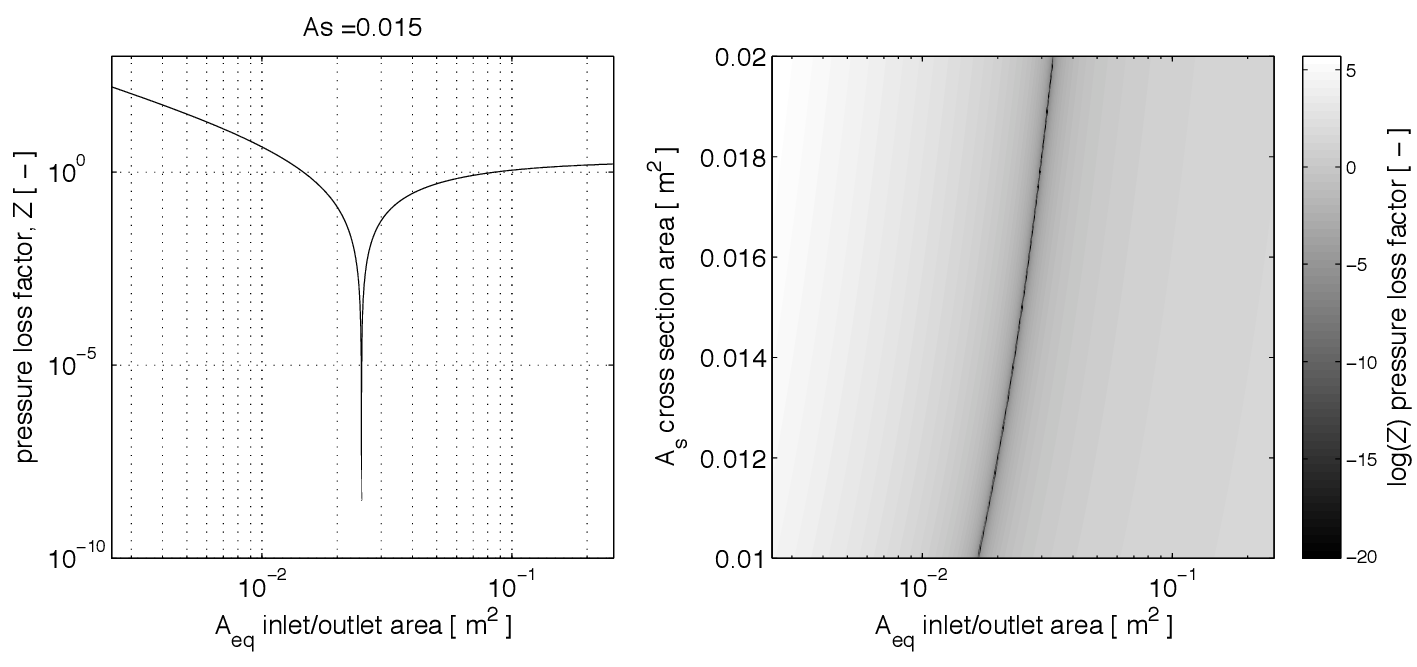
\includegraphics[width=0.9\textwidth, height=0.9\textheight, keepaspectratio=true]{media/PressureLossFactor.png}
	\caption{Pressure loss factor, Z, as a function of $A_{eq}$ at $A_s = 0.015m^2$; and (b) surface plot of Z as a function of $A_s$ and $A_{eq}$ for a 1m x 1m window. The minimum follows the predicted ratio of 5/3 between $A_{eq}$ and As. \protect \label{fig:PressureLossFacor}}
\end{figure}

\subsubsection{Screen Heat Flux}
To improve the simulation correlation, correlation coefficients are proposed to the five ventilated layer opening parameters defined in ISO 15099; $A_h$, $A_{top}$, $A_{bot}$, $A_l$, and $A_r$. This model includes two correlation constants, C1 and C2 that are determined based on regression analysis of the measured dataset. An additional two constants, C3 and C4, are also optimized and used to correlate the to left/right and top/bottom gaps respectively as shown in Equations~\ref{eq:ScreenCorrelations}. 

\begin{equation}
\begin{array}{rl}
A_h & = C_1 \cdot d_{surface}^{C_2} \cdot A_w \\
A_{l,r}^* & = C_3 \cdot A_{l,r} \\
A_{t,b}^* & = C_4 \cdot A_{t,b}
\end{array}
\label{eq:ScreenCorrelations}
\end{equation}

Where correlation constants are:

\begin{tabular}{ l c }
	\hline	
	Coefficient & Value \\
	\hline
	\hline
	$C_1$ & 0.078 \\
	$C_2$ & 1.20 \\
	$C_3$ & 1 \\
	$C_4$ & 1 \\
	\hline  
	
\end{tabular}

\subsubsection{Horizontal Louvered Blind}
To improve the simulation correlation, correlation coefficients are proposed to the five ventilated layer opening parameters defined in ISO 15099; Ah, $A_{top}$, $A_{bot}$, $A_l$, and $A_r$. The proposed heat flux model includes parameters for the openness, $d_{surface}$, open area, $A_h$, tilt, $\phi$, and the layer conductivity, k.

\begin{equation}
\begin{array}{rl}
A_h & = D_1 \cdot [d_{surface} (cos\phi)^{D_2}]^{D_3} \cdot A_s \\
d_{surface} & = 1 - \frac{t}{cos(\phi)(p-t)} \\
t^* & = D_4 \cdot w \cdot cos\phi \\
k^* & = d_{surface} \cdot k_c + (1 - d_{surface})k_s \\
d_{top} & = 0 \\
d_{left, right} & = d_{gap} \textit{(for outside mount)} \\
d_{left, right} & = 0 \textit{(for inside mount)} \\
d_{bottom} & = d_{gap} \textit{(for outside mount)} \\
d_{bottom} & = 0 \textit{(for inside mount)} \\
\end{array}
\label{eq:VenetianCorrelations}
\end{equation}

where $t^*$ and $k^*$ are the revised layer thickness and equivalent conductivity and $k_c$ is the conductivity of the gas between slats at the average blind layer temperature.

Where correlation constants are:

\begin{tabular}{ l c c }
	\hline	
	Coefficient & Horizontal Blinds & Vertical Blinds \\
	\hline
	\hline
	$D_1$ & 0.016 & 0.041 \\
	$D_2$ & -0.63 & -0.00 \\
	$D_3$ & 0.53 & 0.270 \\
	$D_4$ & 0.043 & 0.012 \\
	\hline  
	
\end{tabular}

\subsection{Heat Balance Equations for Between-Glass Shading Device}\label{heat-balance-equations-for-between-glass-shading-device}

In EnergyPlus shading devices are allowed between the two glass panes of double glazing and between the two inner glass panes of triple glazing. Figure~\ref{fig:glazing-system-with-two-glass-layers-and-a} shows the case of a between-glass shading device in double glazing.

\begin{figure}[hbtp] % fig 105
\centering
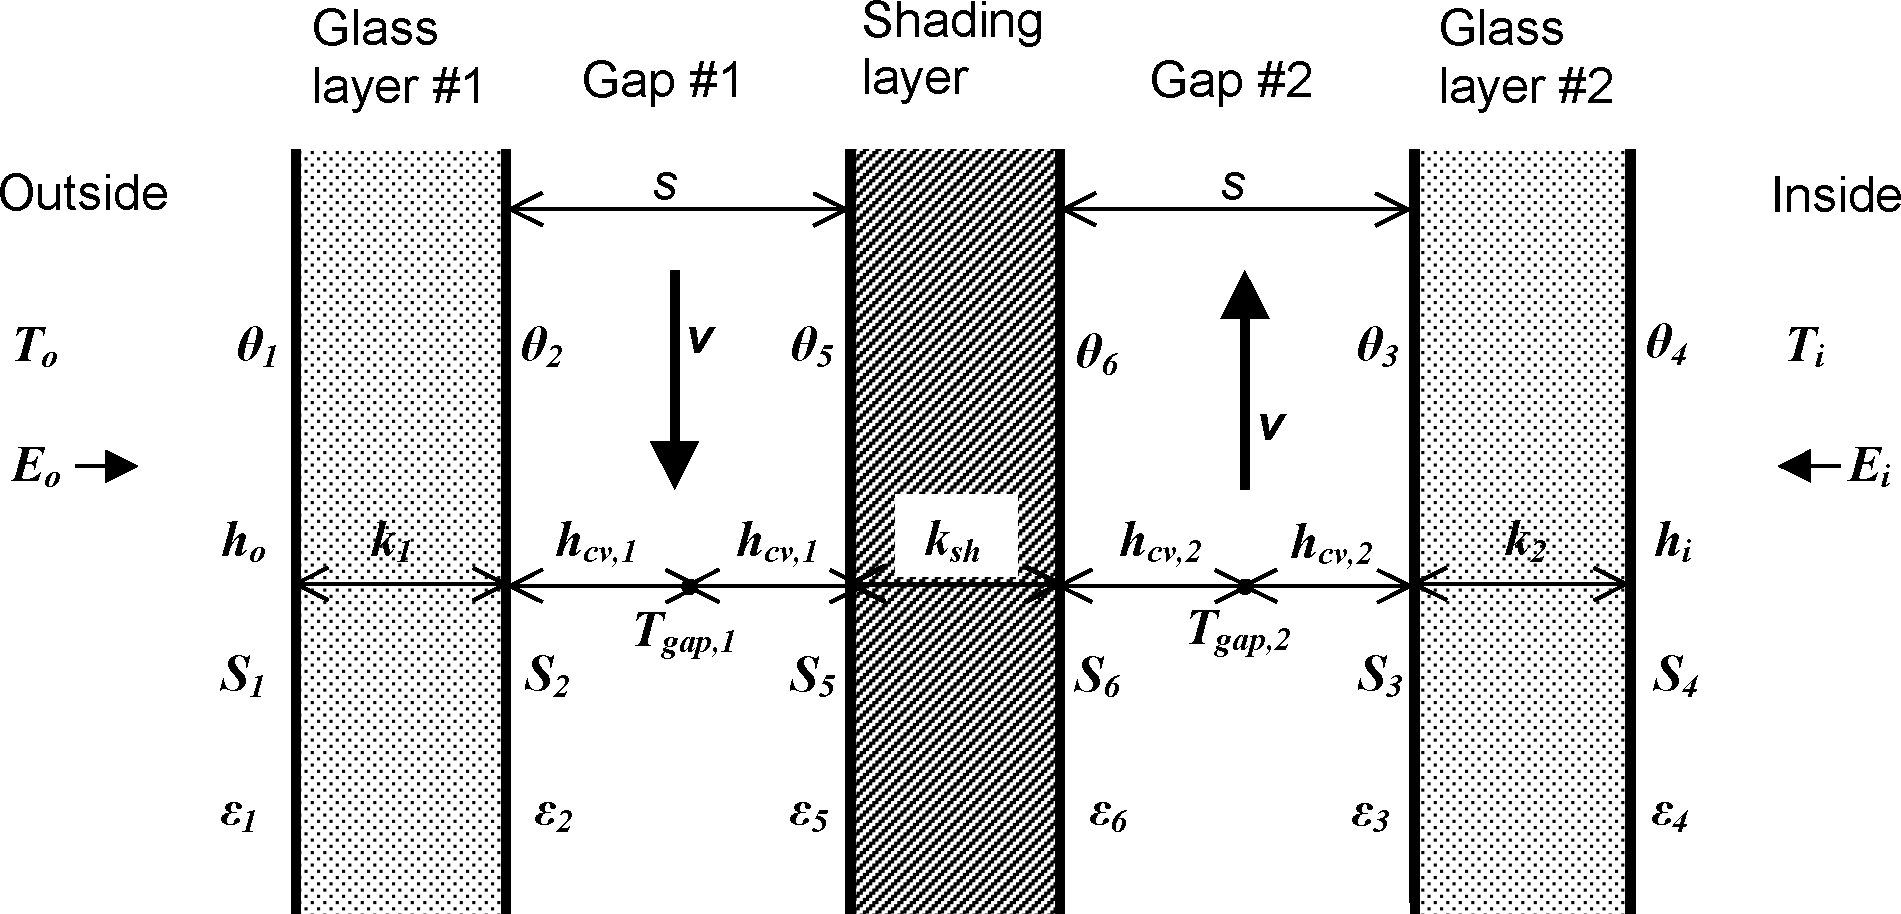
\includegraphics[width=0.9\textwidth, height=0.9\textheight, keepaspectratio=true]{media/image1691.png}
\caption{Glazing system with two glass layers and a between-glass shading device showing variables used in the heat balance equations. \protect \label{fig:glazing-system-with-two-glass-layers-and-a}}
\end{figure}

The heat balance equations for the two glass surfaces facing the shading device are the following.

For face \#2:

\begin{equation}
h_{cv,1} (T_{gap,1}-\theta_2) + k_1 (\theta_1-\theta_2) +
    \frac{\sigma \varepsilon_2}{1-\rho_2 R_1} \left[
      \frac{\tau_{sh}}{1-\rho_6\rho_3} (
        \varepsilon_3 \theta_3^4 + \varepsilon_6\theta_6^4\rho_3
      )
      + \varepsilon_5\theta_5^4 + \varepsilon_2\theta_2^4R_1
    \right]-{\sigma \varepsilon_2 \theta_2^4}+{S_2}=0
\end{equation}

where

\begin{equation}
{R_1} = {\rho_5} + \frac{{\tau_{sh}^2{\rho_3}}}{{1 - {\rho_6}{\rho_3}}}
\end{equation}

\emph{T\(_{gap,1}\)} = effective mean air temperature in gap 1 (K)

\emph{h\(_{cv,1}\)} = convective heat transfer coefficient from glass or shading layer to gas in gap 1 (W/m\(^{2}\)K)

For face \#3:

\begin{equation}
h_{cv,2} (T_{gap,2}-\theta_3) + k_2 (\theta_4-\theta_3) +
    \frac{\sigma \varepsilon_3}{1-\rho_3 R_2} \left[
      \frac{\tau_{sh}}{1-\rho_5\rho_2} (
        \varepsilon_3 \theta_2^4 + \varepsilon_5\theta_5^4\rho_2
      )
      + \varepsilon_6\theta_6^4 + \varepsilon_7\theta_3^4R_2
    \right]-{\sigma \varepsilon_3 \theta_3^4}+{S_3}=0
\end{equation}

where

\begin{equation}
{R_2} = {\rho_6} + \frac{{\tau_{sh}^2{\rho_2}}}{{1 - {\rho_5}{\rho_2}}}
\end{equation}

\emph{T\(_{gap,2}\)} = effective mean air temperature in gap 2 (K)

\emph{h\(_{cv,2}\)} = convective heat transfer coefficient from glass or shading layer to gas in gap 2 (W/m\(^{2}\)K)

The heat balance equations for the shading layer faces are:

For face \#5:

\begin{equation}
h_{cv,1} (T_{gap,1}-\theta_5) + k_sh (\theta_6-\theta_5) +
    \frac{\sigma \varepsilon_5}{1-\rho_2 R_1} \left[
      \frac{\tau_{sh}\rho_2}{1-\rho_5\rho_3} (
        \varepsilon_3 \theta_3^4 + \varepsilon_6\theta_6^4\rho_3
      )
      + \varepsilon_2\theta_2^4 + \varepsilon_5\theta_5^4\rho_2
    \right]-{\sigma \varepsilon_5 \theta_5^4}+{S_5}=0
\end{equation}

For face \#6:

\begin{equation}
h_{cv,2} (T_{gap,2}-\theta_3) + k_2 (\theta_4-\theta_3) +
    \frac{\sigma \varepsilon_3}{1-\rho_3 R_2} \left[
      \frac{\tau_{sh}}{1-\rho_5\rho_2} (
        \varepsilon_2 \theta_2^4 + \varepsilon_5\theta_5^4\rho_2
      )
      + \varepsilon_6\theta_6^4 + \varepsilon_7\theta_3^4R_2
    \right]-{\sigma \varepsilon_3 \theta_3^4}+{S_3}=0
\end{equation}

The convective heat transfer coefficients are given by:

\begin{equation}
  \begin{array}{rl}
    h_{cv,1} &= 2 h_{c,1} + 4v \\
    h_{cv,2} &= 2 h_{c,2} + 4v
  \end{array}
\label{eq:hcv1hcv2Array}
\end{equation}

where

\emph{h\(_{c,1}\),h\(_{c,2}\)} = surface-to-surface heat transfer coefficients for gap \#1 and \#2,~ respectively,~ when these gaps are non-vented (closed).

\emph{v} = air velocity in the gaps (m/s). It is assumed that the gap widths are equal, so that the velocity of flow in the gaps is equal and opposite, i.e., when the airflow is upward in gap \#1 it is downward in gap \#2 and vice-versa.

In analogy to the interior or exterior shading device case, the air velocity is determined by solving the following pressure balance equation:

\begin{equation}
\Delta {p_{T,1,2}} = \Delta {p_{B,1}} + \Delta {p_{HP,1}} + \Delta {p_{Z,1}} + \Delta {p_{B,2}} + \Delta {p_{HP,2}} + \Delta {p_{Z,2}}
\end{equation}

where the driving pressure difference between gap \#1 and \#2 is:

\begin{equation}
\Delta {p_{T,1,2}} = {\rho_0}{T_0}gH\sin \phi \frac{{\left| {{T_{gap,1}} - {T_{gap,2}}} \right|}}{{{T_{gap,1}}{T_{gap,2}}}}{\rm{~~~~~(Pa)}}
\label{eq:DeltapT12Equation}
\end{equation}

The pressure drops on the right-hand side of this equation are:

\begin{equation}
  \begin{array}{rl}
    \Delta p_{B,i} &= \frac{\rho_{gap,i}}{2} v^2 \\
    \Delta p_{HP,i} &= 12 \mu_{gap,i} \frac{H}{s^2} \\
    \Delta p_{Z,i} &= \frac{\rho_{gap,i} v^2}{2}\PB{Z_{in,i} + Z_{out,i}}
  \end{array}
\end{equation}

where \emph{i} = gap number (1 or 2).

It can be shown that \({Z_{in,1}} + {Z_{out,1}} = {Z_{in,2}} + {Z_{out,2}}\) . Then, inserting these pressure drop expressions into Equation~\ref{eq:DeltapT12Equation}, we obtain the following expression for the airflow velocity:

\begin{equation}
v = \frac{{{{\left[ {{{\left( {\frac{{12({\mu_{gap,}}_1 + {\mu_{gap,}}_2)H}}{{{s^2}}}} \right)}^2} + 2\Delta {p_{T,1,2}}({\rho_{gap,1}} + {\rho_{gap,2}})(1 + {Z_{in}} + {Z_{out}})} \right]}^{1/2}} - \frac{{12({\mu_{gap,}}_1 + {\mu_{gap,}}_2)H}}{{{s^2}}}}}{{({\rho_{gap,}}_1 + {\rho_{gap,}}_2)(1 + {Z_{in}} + {Z_{out}})}}
\label{eq:AirFlowVelocityEquation}
\end{equation}

The choice of the sign of the square root term is dictated by the requirement that \(v = 0\) ~if \(\Delta {p_{T,1,2}} = 0\), i.e., \({T_{gap,1}} = {T_{gap,2}}\).

Given \(v\),~we can now calculate \({T_{gap,1}}\) and \({T_{gap,2}}\), which gives \(\Delta {p_{T,1,2}}\). The procedure is as follows. We have:

\begin{equation}
{T_{gap,1,out}} = {T_{ave,1}} - ({T_{ave,1}} - {T_{gap,1,in}}){\xi_1}
\end{equation}

where \({T_{ave,1}} = ({\theta_2} + {\theta_5})/2\) ~and \({\xi_1} = {e^{ - \frac{H}{{{H_{0,1}}}}}}\) ~with \({H_{0,1}} = {\rho_{gap,1}}{C_p}sv/(2{h_{cv,1}})\) . Since \({T_{gap,1,in}} = {T_{gap,2,out}}\)~this gives:

\begin{equation}
{T_{gap,1,out}} = {T_{ave,1}} - ({T_{ave,1}} - {T_{gap,2,out}}){\xi_1}
\end{equation}

Similarly,

\begin{equation}
{T_{gap,2,out}} = {T_{ave,2}} - ({T_{ave,2}} - {T_{gap,1,out}}){\xi_2}
\end{equation}

Solving these simultaneous equations gives:

\begin{equation}
  \begin{array}{rl}
    T_{gap,1,out} &= \frac{T_{ave,1}\PB{1 - \xi_1} + \xi_1 T_{ave,2}\PB{1 - \xi_2}}{1 - \xi_1 \xi_2} \\
    T_{gap,2,out} &= \frac{T_{ave,2}\PB{1 - \xi_2} + \xi_2 T_{ave,1}\PB{1 - \xi_1}}{1 - \xi_1 \xi_2}
  \end{array}
\end{equation}

Using these in:

\begin{equation}
{T_{gap,1}} = {T_{ave,1}} - \frac{{{H_{0,1}}}}{H}\left( {{T_{gap,1,out}} - {T_{gap,2,out}}} \right)
\end{equation}

gives:

\begin{equation}
{T_{gap,1}} = {T_{ave,1}} - \frac{{{H_{0,1}}}}{H}\xi \left( {{T_{ave,1}} - {T_{ave,2}}} \right)
\label{eq:Tgap1Equation}
\end{equation}

with:

\begin{equation}
\xi  = \frac{{(1 - {\xi_1})(1 - {\xi_2})}}{{1 - {\xi_1}{\xi_2}}}
\end{equation}

Similarly, from:

\begin{equation}
{T_{gap,2}} = {T_{ave,2}} - \frac{{{H_{0,2}}}}{H}\left( {{T_{gap,2,out}} - {T_{gap,1,out}}} \right)
\end{equation}

we get:

\begin{equation}
{T_{gap,2}} = {T_{ave,2}} - \frac{{{H_{0,2}}}}{H}\xi \left( {{T_{ave,2}} - {T_{ave,1}}} \right)
\label{eq:Tgap2Equation}
\end{equation}

The overall solution sequence is as follows.~ At start of the iteration process, guess \({T_{gap,1}} = {T_{ave,1}}\)~and \({T_{gap,2}} = {T_{ave,2}}\). Then:

1)~~~~Get \({\rho_{gap,1}},{\rho_{gap,2}},{\mu_{gap,1}},{\mu_{gap,2}}\) using \({T_{gap,1}},{T_{gap,2}}\) .

2)~~~~Get still-air conductances \({h_{c,1}},{h_{c,2}}\) by calling WindowGasConductance and NusseltNumber.

3)~~~~Get \(v\)~from Equation~\ref{eq:AirFlowVelocityEquation}.

4)~~~~Get \({h_{cv,1}},{h_{cv,2}}\) from Equation~\ref{eq:hcv1hcv2Array}.

5)~~~~Get \({T_{ave,1}},{T_{ave,2}}\).

6)~~~~Get \emph{H\(_{o,1}\)}, \emph{H\(_{o,2}\)}, \({\xi_1}\) and \({\xi_2}\).

7)~~~~Get \({T_{gap,1}}\) ,\({T_{gap,2}}\) from Equations~\ref{eq:Tgap1Equation} and~\ref{eq:Tgap2Equation}.

The values \({h_{cv,1}}{\rm{,~}}{h_{cv,2}}{\rm{,~}}{T_{gap,1}}\)~and \({T_{gap,2}}\) are then used in the face heat balance equations to find new values of the face temperatures \({\theta_2}{\rm{,~}}{\theta_3},{\rm{~}}{\theta_5}\) and \({\theta_6}\). These are used in turn to get new values of \({h_{cv,1}}{\rm{,~}}{h_{cv,2}}{\rm{,~}}{T_{gap,1}}\)~and \({T_{gap,2}}\) until the whole iterative process converges.

\subsection{Airflow Windows}\label{airflow-windows}

In airflow windows forced air flows in the gap between adjacent layers of glass. Such windows are also known as ``heat-extract windows'' and ``climate windows.''

Five configurations of airflow windows are modeled (Figure~\ref{fig:gap-airflow-configurations-for-airflow}) that depend on the source and destination of forced air. The allowed combinations of Airflow Source and Airflow Destination are:

InsideAir $\rightarrow$ OutsideAir

InsideAir $\rightarrow$ InsideAir

InsideAir $\rightarrow$ ReturnAir

OutsideAir $\rightarrow$ InsideAir

OutsideAir $\rightarrow$ OutsideAir

\begin{figure}[hbtp] % fig 106
\centering
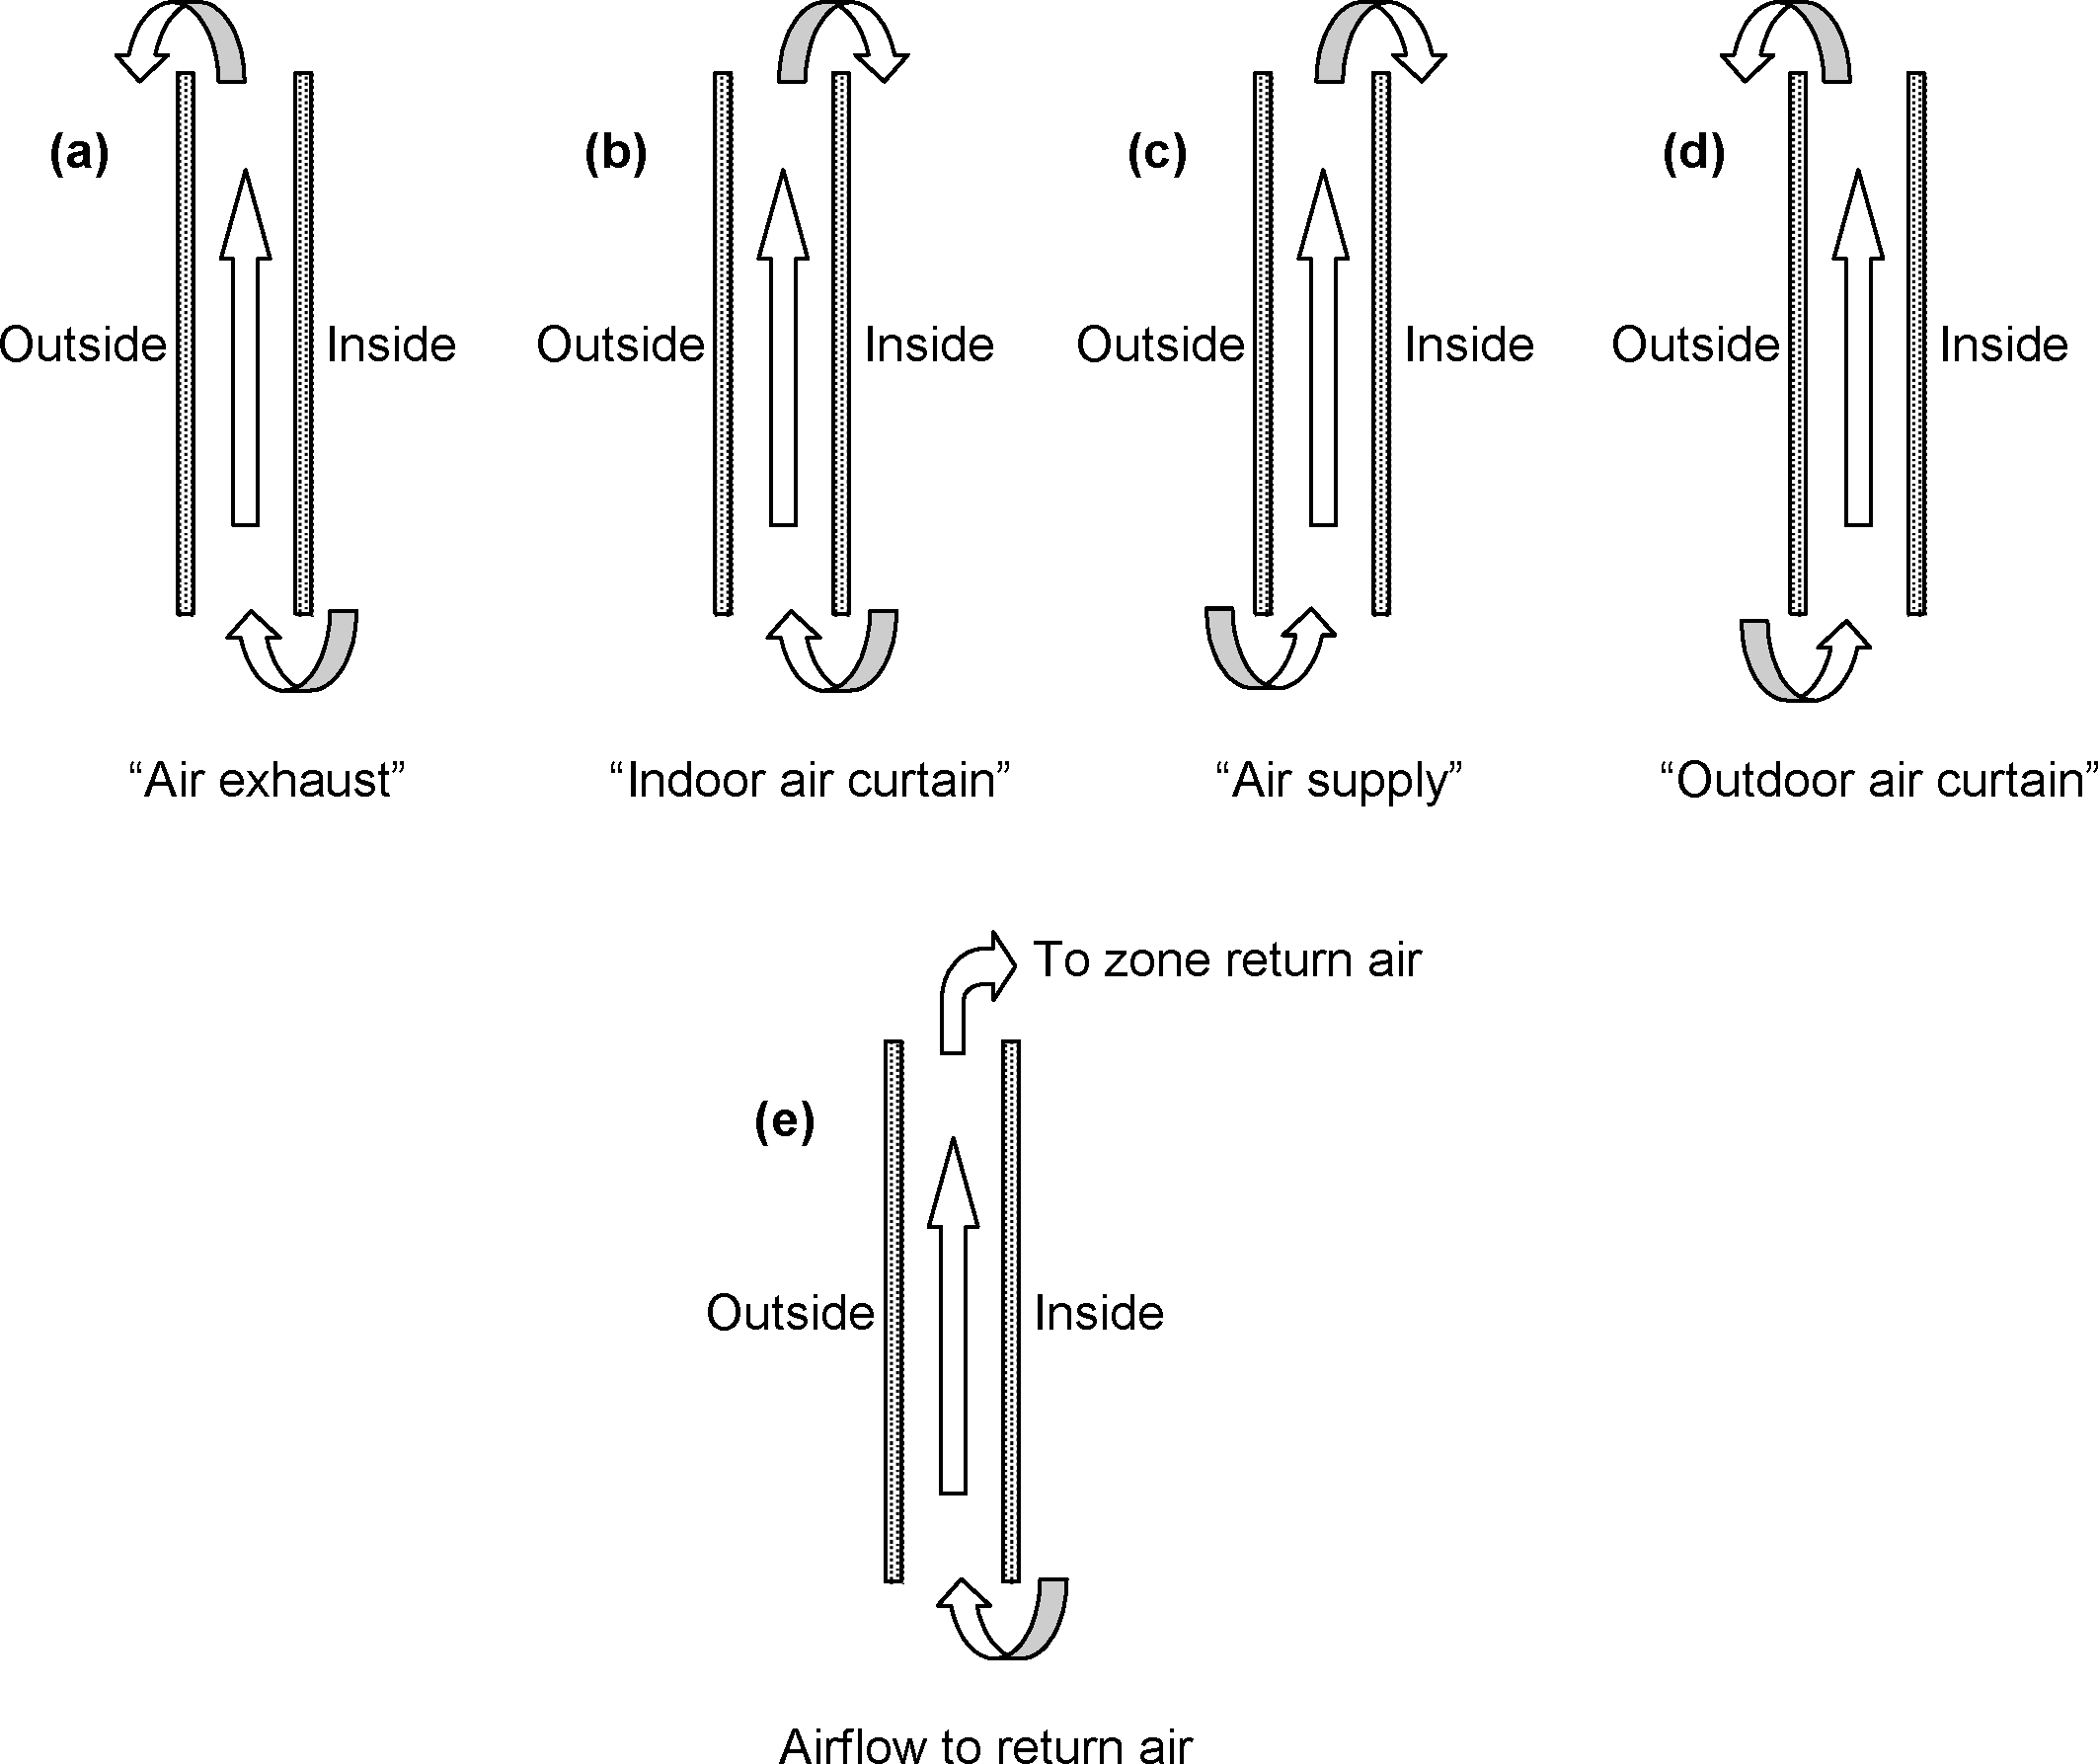
\includegraphics[width=0.9\textwidth, height=0.9\textheight, keepaspectratio=true]{media/image1748.png}
\caption{Gap airflow configurations for airflow windows. From “Active facades,” Version no. 1, Belgian Building Research Institute, June 2002. \protect \label{fig:gap-airflow-configurations-for-airflow}}
\end{figure}

A common application of airflow windows is to reduce the zone cooling load by exhausting indoor air through the window, thereby picking up and rejecting heat from the glazing (Figure~\ref{fig:gap-airflow-configurations-for-airflow}).

Figure~\ref{fig:glazing-system-with-forced-airflow-between} shows the variables used in the heat balance equations for forced airflow in a double-glazed window.

\begin{figure}[hbtp] % fig 107
\centering
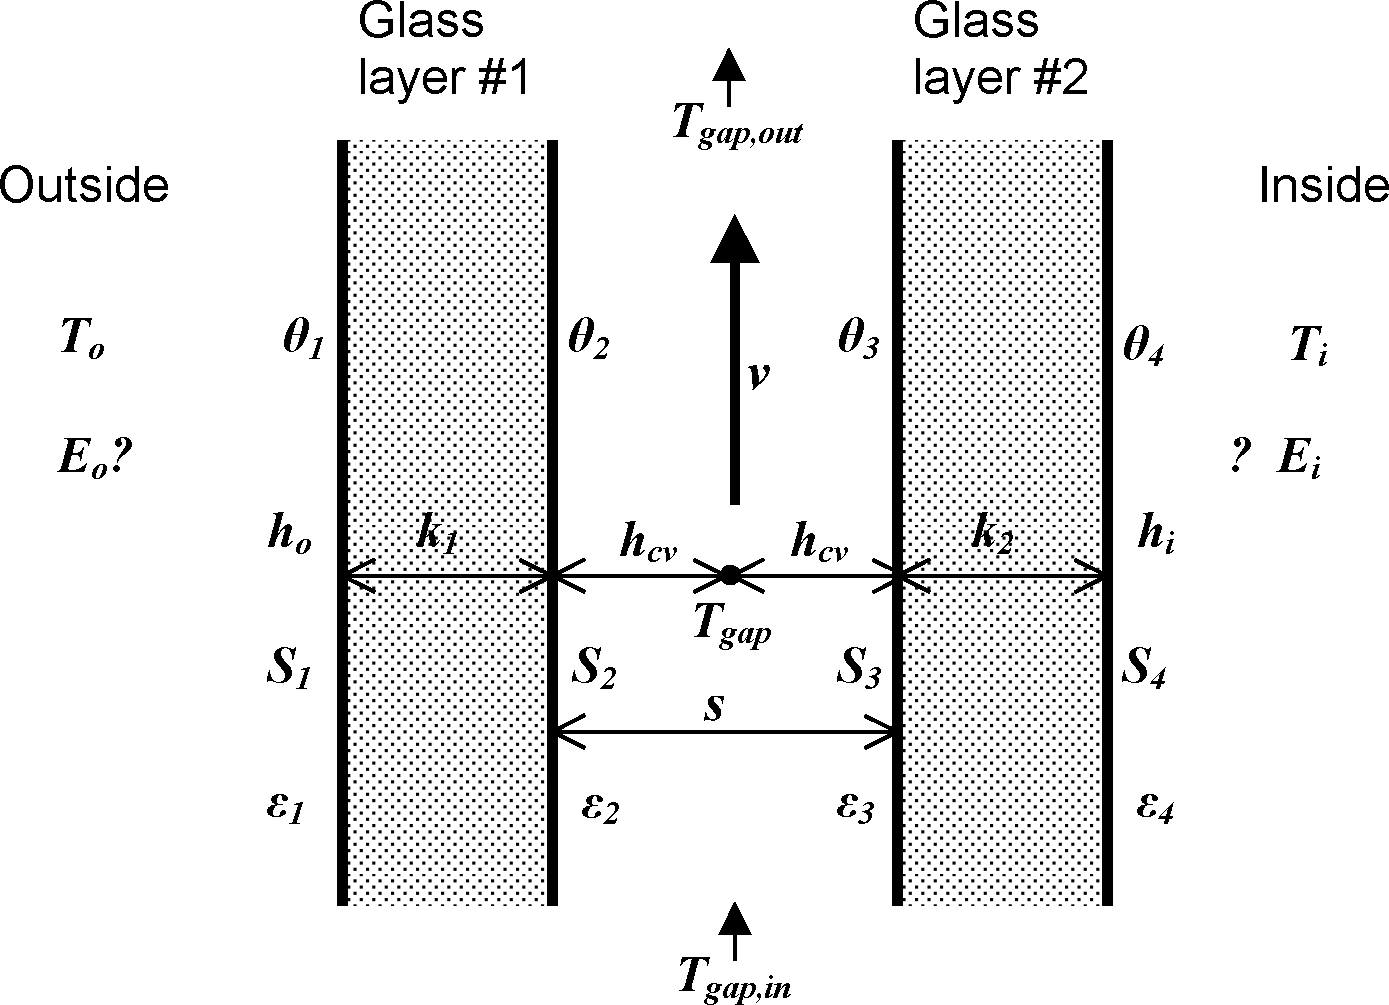
\includegraphics[width=0.9\textwidth, height=0.9\textheight, keepaspectratio=true]{media/image1749.png}
\caption{Glazing system with forced airflow between two glass layers showing variables used in the heat balance equations. \protect \label{fig:glazing-system-with-forced-airflow-between}}
\end{figure}

The heat balance equation for the left-hand glass surface facing the gap in Figure~\ref{fig:glazing-system-with-forced-airflow-between} is:

\begin{equation}
{k_1}({\theta_1} - {\theta_2}) + {h_{cv}}({T_{gap}} - {\theta_2}) + \sigma \frac{{{\varepsilon_2}{\varepsilon_3}}}{{1 - (1 - {\varepsilon_2})(1 - {\varepsilon_3})}}\left( {\theta_3^4 - \theta_2^4} \right) + {S_2} = 0
\end{equation}

The corresponding equation for the right-hand glass surface facing the gap is:

\begin{equation}
{k_2}({\theta_4} - {\theta_3}) + {h_{cv}}({T_{gap}} - {\theta_3}) + \sigma \frac{{{\varepsilon_2}{\varepsilon_3}}}{{1 - (1 - {\varepsilon_2})(1 - {\varepsilon_3})}}\left( {\theta_2^4 - \theta_3^4} \right) + {S_3} = 0
\end{equation}

Here,

\emph{T\(_{gap}\)} = effective mean temperature of the gap air (K)

\emph{h\(_{cv}\)} = convective heat transfer coefficient from glass to gap air (W/m\(^{2}\)K).

The convective heat transfer coefficient is given by:

\begin{equation}
{h_{cv}} = 2{h_c} + 4v
\end{equation}

where

\emph{h\(_{c}\)} = glass-to-glass heat transfer coefficient for non-vented (closed) cavity (W/m\(^{2}\)K)

\emph{v} = mean air velocity in the gap (m/s).

The air velocity is determined by the gap cross-sectional area in the flow direction and the air flow rate, which is an input value that is constant or can vary according to a user-specified schedule:

\begin{equation}
v = \frac{F}{{{A_{gap}}}}{\rm{~~~~~~(m/s)}}
\end{equation}

where

\emph{F} = airflow rate (m\(^{3}\)/s)

\emph{A\(_{gap}\)} = gap cross-sectional area in direction of flow (m\(^{2}\))

It is assumed that the airflow is uniform across the width of the window.

The mean temperature of the gap air is given by the following expression, whose derivation follows that for Equation~\ref{eq:TgapEquation} for the case of an interior shading device:

\begin{equation}
{T_{gap}} = {T_{ave}} - \frac{H}{{{H_0}}}({T_{gap,out}} - {T_{gap,in}})
\end{equation}

where

\begin{equation}
{T_{ave}} = \frac{{{\theta_2} + {\theta_3}}}{2}
\end{equation}

\begin{equation}
{H_0} = \frac{{\rho {C_p}s}}{{2{h_{cv}}}}v
\end{equation}

\emph{H} ~ = glazing height (m)

\emph{T\(_{gap,in}\)} = gap air inlet temperature (\emph{T\(_{i}\)} if the airflow source is indoor air, \emph{T\(_{o}\)} if the airflow source is outside air) (K).

The outlet air temperature is given by:

\begin{equation}
{T_{gap,out}} = {T_{ave}} - ({T_{ave}} - {T_{gap,in}}){e^{ - H/{H_0}}}
\end{equation}

The equations for glass face \#1 and \#4 are the same as those for no airflow in the gap (Equations~\ref{eq:GlazingFace1HeatBalEquation} and~\ref{eq:GlazingFace4HeatBalEquation}).

The convective heat gain to the zone air due to the gap airflow when the airflow destination is indoor air is:

\begin{equation}
{q_v} = \dot m({C_{p,out}}{T_{gap,out}} - {C_{p,i}}{T_i}){\rm{~~~~~~(W)}}
\end{equation}

where

\emph{C\(_{p,i}\)} = heat capacity of the indoor air (J/kg-K)

\emph{C\(_{p,out}\)} = heat capacity of the gap outlet air (J/kg-K)

and where the air mass flow rate in the gap is:

\begin{equation}
\dot m = \rho F{\rm{~~~~~~(kg/s)}}
\end{equation}

\subsubsection{Fan Energy}\label{fan-energy}

The fan energy used to move air through the gap is very small and is ignored.

\subsubsection{Airflow Window with Between-Glass Shading Device}\label{airflow-window-with-between-glass-shading-device}

Figure~\ref{fig:airflow-window-with-between-glass-shading} shows the case of a double-glazed airflow window with a between glass shading device. The heat balance equations in this case are the same as those for the between-glass shading device with natural convection (Figure~\ref{fig:glazing-system-with-two-glass-layers-and-a} and following equations) except that now:

\begin{equation}
v = \frac{{F/2}}{{{A_{gap}}}}{\rm{~~~~~~(m/s)}}
\end{equation}

where \emph{A\(_{gap}\)} = \emph{sW} is the cross-sectional area of the gap on either side of the shading device. It is assumed that the shading device is centered between the two panes of glass so that the airflow, \emph{F}, is divided equally between the two gaps.

The convective heat gain to the zone air due to the airflow through the two gaps when the airflow destination is indoor air is:

\begin{equation}
{q_v} = \dot m({C_{p,ave,out}}{T_{gap,ave,out}} - {C_{p,i}}{T_i}{\rm{)      (W)}}
\end{equation}

where the average temperature of the two outlet air streams is:

\begin{equation}
{T_{gap,ave,out}}{\rm{ =  }}({T_{gap,1,out}} + {T_{gap,2,out}})/2
\end{equation}

and

\emph{C\(_{p,ave,out}\)} = heat capacity of the outlet air evaluated at \emph{T\(_{gap,ave,out}\)} (J/kg-K)

\begin{figure}[hbtp] % fig 108
\centering
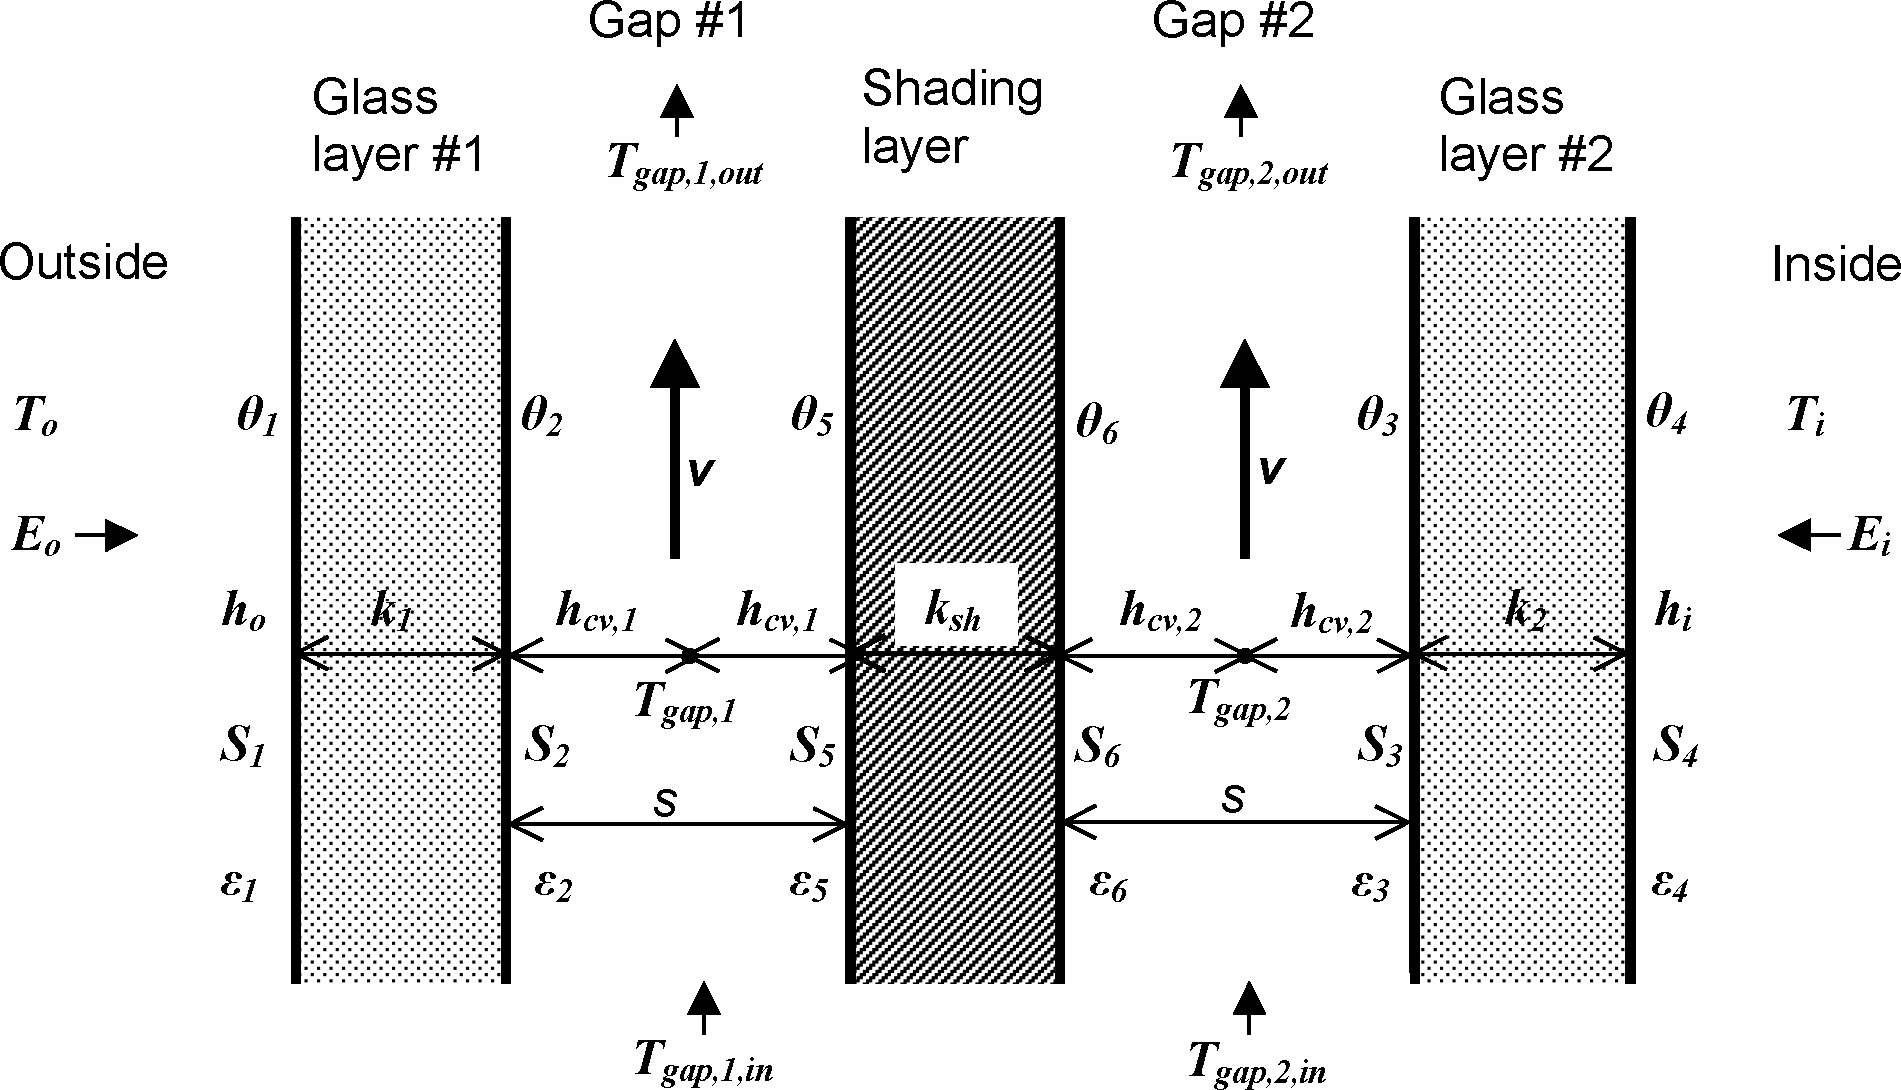
\includegraphics[width=0.9\textwidth, height=0.9\textheight, keepaspectratio=true]{media/image1763.png}
\caption{Airflow window with between-glass shading device showing variables used in the heat balance equations. \protect \label{fig:airflow-window-with-between-glass-shading}}
\end{figure}

\subsection{Evacuated Glazing Unit (EGU)}\label{evacuated-glazing-unit-egu}

Evacuated glazing Units (EGU) are an emerging technology, developed as a concept some 20-30 years ago, but only now approaching wide-spread commercialization and adoption.

\subsubsection{Evacuated glazing unit (EGU): cavity thermal conductance}\label{evacuated-glazing-unit-egu-cavity-thermal-conductance}

Thermal Conductance of the space in an evacuated glazing unit (EGU) is the sum of the conductance of the low pressure gas (air) and radiation conductance.

\begin{equation}
{C_{gas}} = {C_{COND}} + {C_{RAD}}
\end{equation}

\textbf{Conductance of the low-pressure gas}

Conductance of low pressure gasses is calculated using formula by Corrucini (Corruccini, R. (1959)).

\begin{equation}
{C_{COND}} = \alpha  \cdot \left[ {\frac{{\gamma  + 1}}{{\gamma  - 1}}} \right] \cdot {\left[ {\frac{R}{{8 \cdot \pi  \cdot M \cdot T}}} \right]^{\frac{1}{2}}} \cdot P
\end{equation}

\begin{equation}
B = \alpha  \cdot \left[ {\frac{{\gamma  + 1}}{{\gamma  - 1}}} \right] \cdot {\left[ {\frac{R}{{8 \cdot \pi  \cdot M \cdot T}}} \right]^{\frac{1}{2}}}
\end{equation}

\begin{equation}
{C_{COND}} = B \cdot P
\end{equation}

Where:

\begin{equation}
\alpha  = \frac{{{\alpha_1}{\alpha_2}}}{{{\alpha_2} + {\alpha_1}\left( {1 - {\alpha_2}} \right)}}
\end{equation}

$\alpha$\(_{1}\), $\alpha$\(_{2}\) = Accommodation coefficients of the gas molecules with the two surfaces.~ These values depend on the temperature, surface conditions, etc.~ For the present configuration and conditions, it is expected that \emph{$\alpha$} is approximately 0.5.~ If a conservative value is needed, then a value of 1.0 could be used.~ With $\alpha$\(_{1}\), $\alpha$\(_{2}\) = 0.5, $\alpha$ = 0.333.

$\gamma$ = Specific heat ratio, $\gamma$\(_{air}\) = 1.40.

\emph{R} = Universal gas constant, \emph{R} = 8,314.462175 J/mol·K

\emph{M} = Molecular Weight, \emph{M}\(_{air}\) = 28.97 {[}mol/g{]}

\emph{T} = (\emph{T}\(_{1}\) + \emph{T}\(_{2}\))/2 {[}K{]}

\emph{P} = Pressure of the gas {[}N/m\(^{2}\){]}

From the paper Collins and Robinson (Collins, R., \& Robinson, S. (1991)), B is set at approximately 50 for Air, if pressure is given in torr.~ Therefore according to Collins and Robinson, for air and approximate conditions of EGU:

\begin{equation}
  C_{COND} \approx 50 \cdot P
\end{equation}

Where P is in torr (i.e., mm Hg).

\emph{Note: Conversion from Pa to torr is accomplished by multiplying value in torr by 133.28.}

Using formula 2 and assuming \emph{T}\(_{1}\) to be 20\(^{o}\)C and \emph{T}\(_{2}\) to be -18\(^{o}\)C (expected temperatures of glass surfaces in EGU, if one glass surface is low-e and unit is exposed to NFRC standard environmental conditions), and using SI system of units, the B is calculated as 54.4, which is very close to the value of 50, proposed by Collins and Robinson:

\begin{equation}
  C_{COND} \approx 54.4 \cdot P
\end{equation}

EnergyPlus uses an exact value, calculated by the formula, so these values will be input into the calculations, enabling a more flexible model that can account for special treatment of glass surfaces.

\subsubsection{Radiation conductance}\label{radiation-conductance}

Radiation conductance for the two parallel plates is given by:

\begin{equation}
{C_{RAD}} = \frac{1}{{{\varepsilon_1}^{ - 1} + {\varepsilon_2}^{ - 1} - 1}}\sigma \frac{{\left( {{T_1}^4 - {T_2}^4} \right)}}{{{T_1} - {T_2}}}
\label{eq:RadiationConductanceEquation}
\end{equation}

Where:

$\varepsilon$\(_{1}\) = emissivity of the first facing glass surface, {[} - {]}

$\varepsilon$\(_{2}\) = emissivity of the second facing glass surface, {[} - {]}

\(\sigma\) = Stefan-Boltzmann Constant, 5.67 x 10\(^{8}\), {[}W/(m\(^{2}\)·K\(^{4}\)){]}

T\(_{1}\)~~ = Temperature of the first facing glass surface, {[}K{]}

T\(_{2}\)~~ = Temperature of the second facing glass surface. {[}K{]}

Assuming glass surface temperatures of 20\(^{o}\)C and -18\(^{o}\)C, respectively, the following radiation conductances are obtained for the three different glass emissivities:

Clear Glass ($\varepsilon$\(_{1}\) = $\varepsilon$\(_{2}\) = 0.84): C\(_{RAD}\) = 3.4 W/m\(^{2}\)K

Hard Coat Low-e ($\varepsilon$\(_{1}\) or $\varepsilon$\(_{2}\) = 0.15): C\(_{RAD}\) = 0.68 W/m\(^{2}\)K

Soft Coat Low-e ($\varepsilon$\(_{1}\) or $\varepsilon$\(_{2}\) = 0.04): C\(_{RAD}\) = 0.19 W/m\(^{2}\)K

\textbf{\emph{Note:}} \emph{C\(_{RAD}\) of 0.09 is theoretically possible using the best low-e technology of present day (i.e.,} \emph{$\varepsilon$\(_{1}\) or} \emph{$\varepsilon$\(_{2}\) = 0.02).}

\textbf{\emph{Note:}} \emph{Low-e values above are typical values, which will vary by manufacturer.~ Some more recent hard coat low-e values are at or below 0.1.}

It should also be noted that values above are based on the fix set of temperatures, while in reality temperatures will depend on the environmental conditions and surface emissivities (e.g., it cannot be expected that clear glass will have same \emph{T\(_{1}\)} and \emph{T\(_{2}\)} as low-e glass).

Equation~\ref{eq:RadiationConductanceEquation} is a precise formulation for two parallel plates at the constant temperature.~ A simplified equation under these conditions is given in the form of:

\begin{equation}
{C_{RAD}} = 4\sigma \frac{1}{{{\varepsilon_1}^{ - 1} + {\varepsilon_2}^{ - 1} - 1}}{T_m}^3
\end{equation}

Where:

\emph{T\(_{m}\)} = mean temperature, {[}K{]}

\begin{equation}
{T_m} = \frac{{\left( {{T_1} + {T_2}} \right)}}{2}
\end{equation}

Calculation of the U-factor:

\begin{equation}
U = \frac{1}{{{R_{tot}}}} = \frac{1}{{{R_o} + 2 \cdot {R_{glass}} + {R_{gap}} + {R_i}}}
\end{equation}

\begin{equation}
{R_{gap}} = \frac{1}{{{C_{gap}}}} = \frac{1}{{{C_{COND}} + {C_{RAD}}}}
\end{equation}

\begin{equation}
{R_{glass}} = \frac{{{t_{glass}}}}{{{k_{glass}}}}
\end{equation}

Where:

\emph{t}\(_{glass}\) = glass thickness; {[}m{]}

\emph{k}\(_{glass}\) = glass conductivity; \emph{k}\(_{glass}\) = 1 W/(m·K)

\emph{R}\(_{glass}\) = 0.003 m\(^{2}\)K/W (for 3 mm glass pane)

\emph{R}\(_{o}\) $\approx$ 0.033 m\(^{2}\)K/W

\emph{R}\(_{i}\) $\approx$ 0.14 m\(^{2}\)K/W

U-factor of EGU without any pillars (pretending that this is possible) would be calculated using \emph{C}\(_{RAD}\) only.~ From above radiation conductance calculations:

\emph{Clear Glass: ~~~~~~~~~~ U = 2.64 W/(m\(^{2}\)·K) {[}0.464 Btu/(hr·ft\(^{2}\)·ºF){]}}

\emph{Hard Coat Low-e: ~~~ U = 0.62 W/(m\(^{2}\)·K) {[}0.109 Btu/(hr·ft\(^{2}\)·ºF){]}}

\emph{Soft Coat Low-e:~~~~~ U = 0.19 W/(m\(^{2}\)·K) {[}0.034 Btu/(hr·ft\(^{2}\)·ºF){]}}

Adding conductance of the air at 0.001 torr (\emph{C}\(_{COND}\) = 0.08 W/(m\(^{2}\)·K), these values become:

\emph{Clear Glass: ~~~~~~~~~~ U = 2.66 W/(m\(^{2}\)·K) {[}0.468 Btu/(hr·ft\(^{2}\)·ºF){]}}

\emph{Hard Coat Low-e: ~~~ U = 0.68 W/(m\(^{2}\)·K) {[}0.120 Btu/(hr·ft\(^{2}\)·ºF){]}}

\emph{Soft Coat Low-e:~~~~~ U = 0.27 W/(m\(^{2}\)·K) {[}0.048 Btu/(hr·ft\(^{2}\)·ºF){]}}

In contrast, the U-factor of the same configuration with the air at atmospheric pressure will be (For the space width of 50 mm, C\(_{COND}\) ≈ 450 W/m\(^{2}\)K):

\emph{Clear Glass: ~~~~~~~~~~ U = 5.52 W/(m\(^{2}\)·K) {[}0.468 Btu/(hr·ft\(^{2}\)·ºF){]}}

\emph{Hard Coat Low-e: ~~~ U = 5.52 W/(m\(^{2}\)·K) {[}0.120 Btu/(hr·ft\(^{2}\)·ºF){]}}

\emph{Soft Coat Low-e:~~~~~ U = 5.52 W/(m\(^{2}\)·K) {[}0.048 Btu/(hr·ft\(^{2}\)·ºF){]}}

It is clear that emissivity of the glass surface makes no difference, because of the dominant conductance of the air space.~ Also, it is worth noting that the U-factor of such configuration is very close to the U-factor of single glazing.

\subsubsection{Evacuated glazing unit (EGU): Glass support element thermal conductance}\label{evacuated-glazing-unit-egu-glass-support-element-thermal-conductance}

Glass panes in the EGU are separated by an array of small support elements.~ Typically, these support elements have a cylindrical shape and are often referred to as ``pillars.''~ Typical geometry of the pillar is 0.5-1.0 mm diameter and 0.05 mm (50 mm) height.~ They are typically spaced 1-2 in. apart in a form of square or staggered matrix.

\subsubsection{Calculation of the U-factor}\label{calculation-of-the-u-factor}

The conductance of these elements can be measured or numerically modeled to determine accurate thermal performance.~ Approximate method also exists and is based on the combination of modeling and analytical work for the conduction through small cylinders in contact with infinite parallel plates with thickness much larger than cylinder height.

The following formula can be used to determine conductance of the single pillar, \emph{C}\(_{p}\) (Collins and Fisher-Cripps 1991):

\begin{equation}
{C_p} = \frac{{2ka}}{{1 + \frac{{2h}}{{\pi a}}}}
\end{equation}

Where:

\emph{k}~~~ = conductivity of glass, W/(m·K)

\emph{a}~~~ = radius of the pillar (m)

\emph{h}~~~ = pillar height, m

For the square array of support pillars (Collins and Fischer-Cripps 1991) proposes the following formula for their conductance, \emph{C}\(_{pa}\):

\begin{equation}
{C_{pa}} = \frac{{2ka}}{{{\lambda ^2}\left( {1 + \frac{{2h}}{{\pi a}}} \right)}}
\end{equation}

Where:

$\lambda$ = pillar spacing, m

This formula is approximate and does not include effect of the conductivity of the pillar, but it gives good approximation for common materials used in this technology, since conductivity of the pillar does not play substantial role for non-insulating pillars (where ``non-insulating'' would mean that conductivity of the pillar is equal or higher than the conductivity of the glass pane.

The U-factor of the EGU with support pillars is then:

\begin{equation}
U = \frac{1}{{{R_{tot}}}} = \frac{1}{{{R_o} + 2 \cdot {R_{glass}} + {R_{gap}} + {R_i}}}
\end{equation}

Where:

\begin{equation}
{R_{gap}} = \frac{1}{{{C_{gap}}}} = \frac{1}{{{C_{COND}} + {C_{RAD}} + {C_{pa}}}}
\end{equation}

\subsubsection{References}\label{references-055}

Collins, R., \& Fischer-Cripps, A. 1991. ``Design of Support Pillar Arrays in Flat Evacuated Windows.''. Aust. J. Phys.

Collins, R., \& Robinson, S. 1991. \emph{``Evacuated Glazing''.} Solar Energy. Vol. 47, No. 1, pp.~27-38.

Corruccini, R. 1959. ``Gaseous Heat Conduction at Low Pressures and Temperatures''. Vacuum. Vol. 7-8, pp.19-29.

\subsection{Thermal Performance of Deflected Insulated Glazing Unit (IGU)}\label{thermal-performance-of-deflected-insulated-glazing-unit-igu}

\subsubsection{Introduction}\label{introduction-002}

Deflection of insulated glazing unit (IGU) can result in thermal performance degradation or improvement due to the reduction or increase of gap space width. Convection of the gas fill is affected by changed gap space and due to modified convection pattern and shorter or longer thermal path at the center of the glazing unit can result in increased or decreased thermal performance. For the most part, U-factor is mostly affected as a direct result of changed thermal performance; however note that solar heat gain through the window (SHGC) can also be affected because of the effect of inward flowing fraction of absorbed solar radiation, which is affected by thermal performance of the IGU.

Deflection in sealed IGU is caused by the difference in gas pressure in IGU gap vs.~outdoor/indoor pressure. Indoor and outdoor pressure can be considered equal, since indoor building environment is in pretty good contact with outdoor environment. We will call this pressure an atmospheric pressure, \emph{P\(_{a}\)}. The differences in pressure between atmospheric and gap pressure is due to several factors, listed here:

1)~~~Difference in atmospheric pressure between IGU fabrication location and end use location

2)~~~Difference in temperature during fabrication and actual operating conditions for the glazing. It should be noted that initial temperature can be higher than ambient temperature during fabrication process, due to elevated sealant temperatures, which can raise local temperatures within the IGU.

3)~~~Unbalanced gas fill leakage through the sealants, resulting in lower gap pressure and inward deflection.

4)~~~Wind or static load pressure

Effects 1 and 2 will be modeled using equations presented below, while effect 3 does not have credible mathematical model. However, cumulative deflection, resulting from all three effects can be measured in the field and its effect on thermal performance can be modeled by specifying center glazing deflection.

Wind or static load pressure effects on deflection is not included in this model at this time, but will be considered for future versions.

Recognizing that indoor and outdoor air pressure could be different, such as in hot box test environment, future plans for the extension of the model will include option to specify different values for indoor and outdoor pressure. Another future improvement to the model will also include linking certain air gaps with indoor or outdoor environment, meaning that respective pressures in linked spaces will be set to equal.

\subsubsection{Mathematical Model}\label{mathematical-model-000}

Mathematical model described in detail here is based on the research work by Bernier and Bourret (1997) and Timoshenko and Woinowsky-Krieger (1959). Bernier and Bourret (1997) of the Ecole Polytechnique Montréal adopted Timoshenko and Woinowsky-Krieger (1959) model for calculating flat plate deflection subjected to the differential pressure field (static), while their original contribution was to develop correlations for changes in thermal performance, based on IGU deflection at the center of glazing location. In addition to adopting Bernier and Bourret (1997) model here, we have also developed model for calculating change in thermal performance of deflected units when this deflection is measured in the field. Therefore, the mathematical formulation, presented here is divided into two sections; 1) calculation of the deflection and resulting thermal performance caused by pressure and temperature effects and 2) calculation of the thermal performance of the IGU when the deflection is measured.

\subsubsection{Calculation of the deflection and thermal performance caused by pressure and temperature effects}\label{calculation-of-the-deflection-and-thermal-performance-caused-by-pressure-and-temperature-effects}

If coordinate system is set as shown in Figure~\ref{fig:deflection-coordinate-system-2d} and Figure~\ref{fig:deflection-coordinate-system-3d}, it is possible to calculate deflection distribution at each point of pane by using following equation:

\begin{figure}[hbtp] % fig 109
\centering
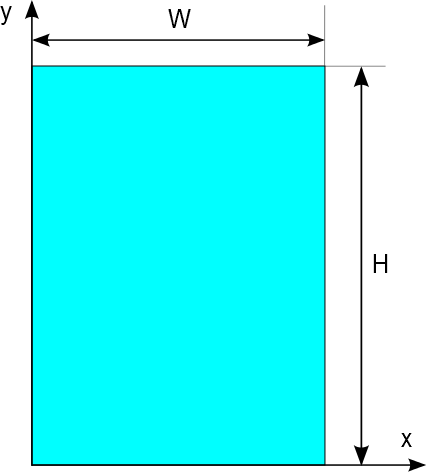
\includegraphics[width=0.9\textwidth, height=0.9\textheight, keepaspectratio=true]{media/image1779.png}
\caption{Deflection Coordinate System - 2D \protect \label{fig:deflection-coordinate-system-2d}}
\end{figure}

\begin{equation}
{L_{D\left( i \right)}}\left( {x,y} \right) = \frac{{16\cdot \Delta {P_{\left( i \right)}}}}{{{\pi ^6}\cdot {D_{\left( i \right)}}}}\mathop \sum \limits_{m = 1,3,5 \ldots }^\infty  \mathop \sum \limits_{n = 1,3,5 \ldots }^\infty  \frac{{\sin \frac{{m\pi x}}{W}\sin \frac{{n\pi y}}{H}}}{{mn{{\left( {{{\left( {\frac{m}{W}} \right)}^2} + {{\left( {\frac{n}{H}} \right)}^2}} \right)}^2}}}
\label{eq:IGUDeflection}
\end{equation}

where

\begin{equation}
{D_{\left( i \right)}} = \frac{{E\cdot t_{\left( i \right)}^3}}{{12\cdot \left( {1 - {\nu ^2}} \right)}}
\label{eq:IGUDiDeflection}
\end{equation}

and

\emph{E} = Young's modulus (7.2 x 10\(^{10}\)) {[}Force per unit Area; SI: Pa, IP: psi{]}

\emph{t} = thickness of glazing pane {[}Length; SI: m, IP: in.{]}

$\nu$ = poison's ratio (0.22 for glass) {[}Non-Dimensional{]}

\begin{figure}[hbtp] % fig 110
\centering
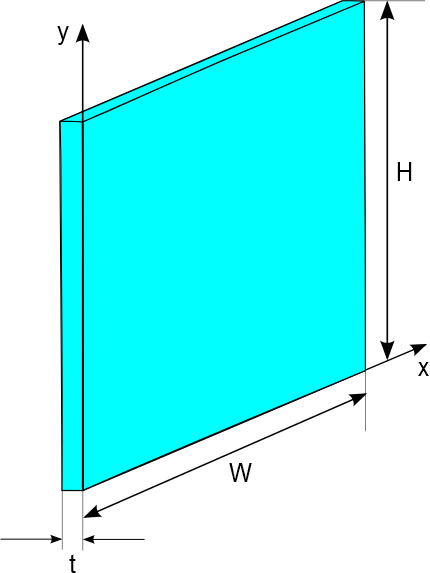
\includegraphics[width=0.9\textwidth, height=0.9\textheight, keepaspectratio=true]{media/image1782.png}
\caption{Deflection Coordinate System - 3D \protect \label{fig:deflection-coordinate-system-3d}}
\end{figure}

\begin{equation}
\emph{\(\Delta\)P\(_{i}\)} = \emph{P\(_{gap(i)}\)} - \emph{P\(_{gap(i-1)}\)} (for~i-th~pane) {~~[}Force~per~unit~Area;~SI:~Pa,~IP:~psi{]}
\label{eq:IGUdPiIthPane}
\end{equation}

\begin{equation}
\emph{\(\Delta\)P\(_{i}\)} = \emph{P\(_{gap(1)}\)} - \emph{P\(_{a}\)} (first~pane) {~~[}Force~per~unit~Area;~SI:~Pa,~IP:~psi{]}
\label{eq:IGUdPiFirstPane}
\end{equation}

\begin{equation}
\emph{\(\Delta\)P\(_{i}\)} = \emph{P\(_{a}\) - P\(_{gap(n-1)}\)} (last~pane) {~~[}Force~per~unit~Area;~SI:~Pa,~IP:~psi{]}
\label{eq:IGUdPiLastPane}
\end{equation}

where

\emph{P\(_{a}\) =} atmospheric pressure. {[}Force per unit Area; SI: Pa, IP: psi{]}

\begin{equation}
{P_{gap\left( i \right)}} = \frac{{{P_{ini}}{V_{ini\left( i \right)}}{T_{gap\left( i \right)}}}}{{{T_{ini}}{V_{gap\left( i \right)}}}}
\end{equation}

where

\emph{P\(_{ini}\)} = Initial pressure. Applies to all gaps as a single value (input data - measured or otherwise) {[}Force per unit Area; SI: Pa, IP: psi{]}

\emph{T\(_{ini}\)} = Initial temperature. Applies to all gaps as a single value (input data - measured or otherwise) {[}Degree Temperature; SI: K, IP: R{]}

\emph{V\(_{ini(i)}\)} = Initial volume for i-th gap. {[}Length*Length*Length; SI: m\(^{3}\), IP: in\(^{3}\){]}

\begin{equation}
{V_{ini\left( i \right)}} = {L_i}\cdot W\cdot H
\end{equation}

where

\emph{L\(_{i}\)} = non-deflected glazing gap width (for i-th gap) {[}Length; SI: m, IP: in.{]}

\emph{W} = IGU width {[}Length; SI: m, IP: in.{]}

\emph{H} = IGU height {[}Length; SI: m, IP: in.{]}

\emph{T\(_{gap(i)}\)} = temperature of the gap between two glass panes (calculated using center of glazing thermal calculation algorithm, as described in ISO 15099 (ISO 2003). This value is first calculated using non-deflected state and is recalculated after the resulting deflection is calculated. This process is repeated until temperature at next iteration does not differ by more than 0.1 ºC

\emph{V\(_{gap(i)}\)} = volume of the IGU gap in deflected state {[}Lentgh*Length*Length; SI: m\(^{3}\), IP: in\(^{3}\){]}

\begin{equation}
{V_{gap\left( i \right)}} = {V_{ini\left( i \right)}} + W\cdot H\cdot \left( {\overline {{L_{D,i}}}  - \overline {{L_{D,i + 1}}} } \right)
\label{eq:IGUGapVolume}
\end{equation}

where

\(\overline {{L_{D,i}}}\) ~is mean deflection value for i-th pane. {[}Length; SI: m, IP: in.{]}

Deflection of each pane can be positive or negative and is done solely to establish reference. Current frame of reference is that positive deflection means that pane is deflecting towards left side, while negative deflection means that pane is deflecting towards right side (see Equation~\ref{eq:IGUGapVolume}). Whether the deflection is in the direction of reducing the gap width or increasing it, it will be the result of pressure difference, as described in Equation~\ref{eq:IGUDeflection}. When pressure in the glazing unit is higher than surrounding environmental pressure, the deflection will be towards increasing gap width (i.e., ballooning), while the opposite situation will result in decreasing gap width (i.e., vacuuming)

\begin{figure}[hbtp] % fig 111
\centering
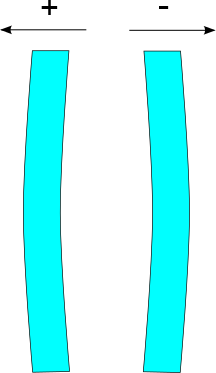
\includegraphics[width=0.9\textwidth, height=0.9\textheight, keepaspectratio=true]{media/image1787.png}
\caption{Deflection Direction Convention \protect \label{fig:deflection-direction-convention}}
\end{figure}

The important part of calculating deflection of the IGU is to determine mean deflection value for each glazing pane. Mean deflection value is used to calculate gap volume in deflected state (see Equation~\ref{eq:IGUGapVolume}). Mean deflection of glazing pane can be calculated by integrating Equation~\ref{eq:IGUDeflection}:

\begin{equation}
\overline {{L_{D\left( i \right)}}}  = \mathop \smallint \limits_{x = 0}^W \mathop \smallint \limits_{y = 0}^H \frac{{16\cdot \Delta {P_{\left( i \right)}}}}{{{\pi ^6}\cdot {D_{\left( i \right)}}}}\mathop \sum \limits_{m = 1,3,5 \ldots }^\infty  \mathop \sum \limits_{n = 1,3,5 \ldots }^\infty  \frac{{\sin \frac{{m\pi x}}{W}\sin \frac{{n\pi y}}{H}}}{{mn{{\left( {{{\left( {\frac{m}{W}} \right)}^2} + {{\left( {\frac{n}{H}} \right)}^2}} \right)}^2}}}
\end{equation}

This is identical to the following expression:

\begin{equation}
\overline {{L_{D\left( i \right)}}}  = \frac{{16\cdot \Delta {P_{\left( i \right)}}}}{{{\pi ^6}\cdot {D_{\left( i \right)}}}}\mathop \sum \limits_{m = 1,3,5 \ldots }^\infty  \mathop \sum \limits_{n = 1,3,5 \ldots }^\infty  \frac{{\mathop \smallint \nolimits_{x = 0}^W \mathop \smallint \nolimits_{y = 0}^H \sin \frac{{m\pi x}}{W}\sin \frac{{n\pi y}}{H}}}{{mn{{\left( {{{\left( {\frac{m}{W}} \right)}^2} + {{\left( {\frac{n}{H}} \right)}^2}} \right)}^2}}}
\end{equation}

and because the integral of sin(x) is equal to --cos(x), the above equation will become:

\begin{equation}
\overline {{L_{D\left( i \right)}}}  = \frac{{16\cdot \Delta {P_{\left( i \right)}}}}{{{\pi ^6}\cdot {D_{\left( i \right)}}}}\mathop \sum \limits_{m = 1,3,5 \ldots }^\infty  \mathop \sum \limits_{n = 1,3,5 \ldots }^\infty  \frac{{\left( {1 - cos\left( {m\pi } \right)} \right)\left( {1 - cos\left( {n\pi } \right)} \right)}}{{mn{{\left( {{{\left( {\frac{m}{W}} \right)}^2} + {{\left( {\frac{n}{H}} \right)}^2}} \right)}^2}}}
\end{equation}

Finally, because \(cos\left( {m\pi } \right)\)~and \(cos\left( {n\pi } \right)\)~values are always equal to -1 for the given range of m and n, the above equation will became:

\begin{equation}
\overline {{L_{D\left( i \right)}}}  = \frac{{16\cdot \Delta {P_{\left( i \right)}}}}{{{\pi ^6}\cdot {D_{\left( i \right)}}}}\mathop \sum \limits_{m = 1,3,5 \ldots }^\infty  \mathop \sum \limits_{n = 1,3,5 \ldots }^\infty  \frac{4}{{{m^2}{n^2}{\pi ^2}{{\left( {{{\left( {\frac{m}{W}} \right)}^2} + {{\left( {\frac{n}{H}} \right)}^2}} \right)}^2}}}
\end{equation}

After calculating the mean pane deflection, the following equation is used to the calculate mean gap width:

\begin{equation}
{L_{r\left( i \right)}} = L + \left( {\overline {{L_{D,\left( i \right)}}}  - \overline {{L_{D,\left( {i + 1} \right)}}} } \right)
\label{eq:IGUMeanPaneDeflection}
\end{equation}

where

\emph{L\(_{r(i)}\)} = Mean gap ``i'' width after incorporating glazing deflection. This mean gap width is used to recalculate thermal performance of deflected IGU.

\(\overline {{L_{D,i}}}\) = mean glazing deflection for each pane ``i''.

Calculation of the deflection at the center of glazing and mean glazing deflection for each pane is an iterative process, where the initial temperature distribution is calculated for non-deflected state, then deflection is calculated based on this temperature distribution, new temperature distribution is calculated for this deflected state, then temperatures from previous iteration are compared to the current iteration and the process is repeated until the difference is no larger than 0.1\(^{o}\)C.

At the end of calculations, program will calculate and return maximum deflection value for each pane (i.e., center of glazing deflection). If we label maximum deflection of each pane as \emph{L\(_{D(i),max}\)}, we can calculate this value by substituting \emph{x} = \emph{W}/2 and \emph{y} = \emph{H}/2 in Equation~\ref{eq:IGUDeflection} to determine deflection at the center point. Therefore:

\begin{equation}
{L_{D\left( i \right),max}} = \frac{{16\cdot \Delta {P_{\left( i \right)}}}}{{{\pi ^6}\cdot {D_{\left( i \right)}}}}\mathop \sum \limits_{m = 1,3,5 \ldots }^\infty  \mathop \sum \limits_{n = 1,3,5 \ldots }^\infty  \frac{{\sin \frac{{m\pi }}{2}\sin \frac{{n\pi }}{2}}}{{mn{{\left( {{{\left( {\frac{m}{2}} \right)}^2} + {{\left( {\frac{n}{2}} \right)}^2}} \right)}^2}}}
\label{eq:IGULDimaxDeflection}
\end{equation}

For glazing systems with more than two glazing layers, meaning multiple gas filled gaps, the deflection will be calculated for each glazing pane assuming that the pressure in a gap is independent from each other and calculated separately, unless spaces are ``linked'' together (e.g., stretched film middle glazing that has hole for equalizing pressure).

\subsubsection{Non-Linked Gaps in 3 or more glazing layer system:}\label{non-linked-gaps-in-3-or-more-glazing-layer-system}

The procedure shown above generally applies to the 3 or more layer glazing system, with the exception that neighboring pressures are no longer \emph{P\(_{a}\)}, but rather could be \emph{P\(_{a}\)} on one side and \emph{P\(_{gap}\)} on the other, or have \emph{P\(_{gap}\)} on both sides, as shown in Figure~\ref{fig:deflection-direction-convention} for gap ``\emph{i}''. Center of glazing thermal calculation will determine new temperature distribution, after deflection is calculated for each glazing and will be used to determine new \emph{P\(_{gap}\)}, as per the procedure above.

\subsubsection{Linked Gaps in 3 or more glazing layer system:}\label{linked-gaps-in-3-or-more-glazing-layer-system}

When one or more gaps are linked together, their pressure is assumed to be identical (e.g., in triple glazing IGU \emph{P\(_{gap,1}\)} = \emph{P\(_{gap,2}\)}).~ This pressure is calculated from temperatures of bounding glazing for linked gaps (e.g., for triple glazing IGU, glazing 1 and 3) and using neighboring pressures outside of those bounding glazing (e.g., for triple glazed IGU, \emph{P\(_{a}\)} on both sides).

\emph{Note: This feature is not implemented in WINDOW 7.1. It is considered for future enhancements to the program.}

\subsubsection{Gap(s) Linked to Indoor or Outdoor Environment:}\label{gaps-linked-to-indoor-or-outdoor-environment}

If one or more glazing gaps are linked to either indoor or outdoor environment its pressure is fixed to \emph{P\(_{a}\)}. In combination situations, such as two or more gaps linked together with one of them being linked to indoor or outdoor environment, they will all have fixed pressure of \emph{P\(_{a}\)}.

\subsubsection{Calculation of the thermal performance caused by measured deflection}\label{calculation-of-the-thermal-performance-caused-by-measured-deflection}

When deflection is measured, it is normally measured at the point of maximum deflection. Maximum deflection occurs at the center of the IGU (at \emph{W}/2 and \emph{H}/2).

Measured value is typically gap width at the point of maximum deflection, which we can label \emph{L\(_{G(i)}\)}. For the i-th measured gap, the width is equal to:

\begin{equation}
{L_{G\left( i \right)}} = {L_{\left( i \right)}} + \left( {{L_{D\left( i \right),max}} - {L_{D\left( {i + 1} \right),max}}} \right)
\label{eq:IGULGiDeflection}
\end{equation}

\begin{figure}[hbtp] % fig 112
\centering
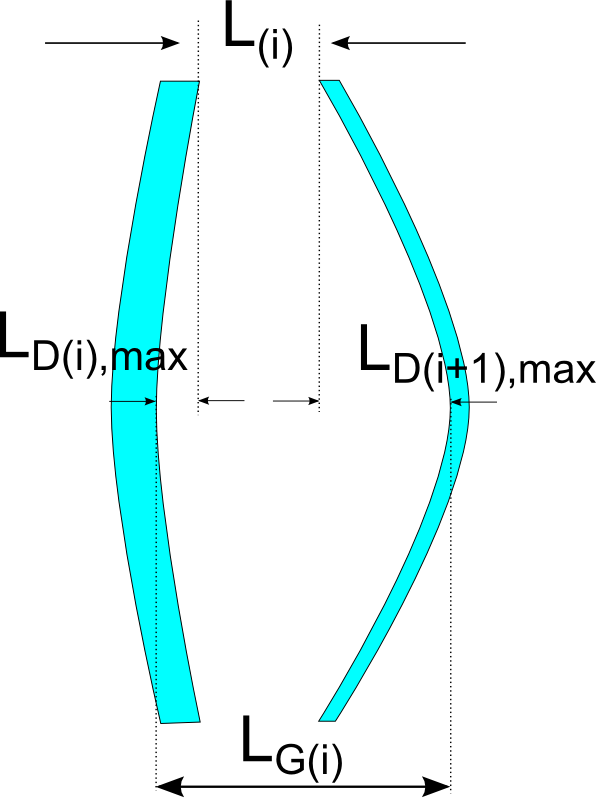
\includegraphics[width=0.9\textwidth, height=0.9\textheight, keepaspectratio=true]{media/image1798.png}
\caption{Sketch of the non-symetrically Deflected Glazing Panes \protect \label{fig:sketch-of-the-non-symetrically-deflected}}
\end{figure}

If we label the ratio of mean deflection and maximum deflection as R\(_{(i)}\), then:

\begin{equation}
{R_{(i)}} = \frac{{\overline {{L_{D(i)}}} }}{{{L_{D(i)}}_{,\max }}} = \sum\limits_{m = 1,3,5,...}^\infty  {\sum\limits_{n = 1,3,5,...}^\infty  {\frac{4}{{{m^2}{n^2}{\pi ^2}{{\left( {{{(\frac{m}{W})}^2} + {{(\frac{n}{H})}^2}} \right)}^2}}}} }
\label{eq:IGUDeflectionRatioi}
\end{equation}

An important thing to note is that the ratios $\PB{R_{\PB{i}}}$\ for all gaps in glazing system are equal.

\begin{equation}
{R_{\left( 1 \right)}} = {R_{\left( 2 \right)}} =  \ldots  = {R_{\left( i \right)}} =  \ldots  = {R_{\left( {n - 1} \right)}} = R
\label{eq:IGUDefletionRatioEquivalency}
\end{equation}

Substituting Equations~\ref{eq:IGUDeflectionRatioi} and~\ref{eq:IGUDefletionRatioEquivalency} into Equation~\ref{eq:IGUMeanPaneDeflection}, the following equation is obtained:

\begin{equation}
{L_{r\left( i \right)}} = {L_{\left( i \right)}} + R\left( {{L_{D\left( i \right),max}} - {L_{D\left( {i + 1} \right),max}}} \right)
\label{eq:IGULriDeflection}
\end{equation}

Combining Equation~\ref{eq:IGULriDeflection} with Equation~\ref{eq:IGULGiDeflection}, we get the following expression for the mean gap width:

\begin{equation}
{L_{r\left( i \right)}} = {L_{\left( i \right)}} + R\left( {{L_{G\left( i \right)}} - {L_{\left( i \right)}}} \right)
\end{equation}

The number of equations given in Equation~\ref{eq:IGULGiDeflection} is equal to n-1, where n is number of panes. Therefore, we need one more equation to complete the system of equations that would allow us to solve for all independent variables. To get the last equation, we can rewrite Equation~\ref{eq:IGULDimaxDeflection} in slightly different manner:

\begin{equation}
{L_{D\left( i \right),max}} = \frac{{\Delta {P_{\left( i \right)}}}}{{{D_{\left( i \right)}}}}\cdot K
\end{equation}

where coefficient K combines all constant terms, while \({D_{\left( i \right)}}\) is given by Equation~\ref{eq:IGUDiDeflection} and \(\Delta {P_{\left( i \right)}}\) is calculated by Equations~\ref{eq:IGUdPiIthPane},~\ref{eq:IGUdPiFirstPane} and~\ref{eq:IGUdPiLastPane}. Summing over all deflections, \({L_{D\left( i \right),max}}\), the following equation is obtained:

\begin{equation}
\mathop \sum \limits_{i = 1}^n \frac{{{D_{\left( i \right)}}}}{K}\cdot {L_{D\left( i \right),max}} = \mathop \sum \limits_{i = 1}^n \Delta {P_{\left( i \right)}} = 0
\end{equation}

Note that sum of all \(\Delta {P_{\left( i \right)}}\) ~is equal to zero since the outside pressure is equal to the inside pressure. Therefore, the remaining equation that completes the set of equations is:

\begin{equation}
\mathop \sum \limits_{i = 1}^n {D_{\left( i \right)}}\cdot {L_{D\left( i \right),max}} = 0
\label{eq:IGUSumDiLDiEq0}
\end{equation}

\subsubsection{Solving system of equations}\label{solving-system-of-equations}

In order to solve this system of equations, we will present Equation~\ref{eq:IGULGiDeflection} in a slightly different manner:

\begin{equation}
0 = {L_{\left( i \right)}} - {L_{G\left( i \right)}} + {L_{D\left( i \right),max}} - {L_{D\left( {i + 1} \right),max}}
\end{equation}

which in developed form will look like this:

\begin{equation}
0 = {L_{\left( 1 \right)}} - {L_{G\left( 1 \right)}} + {L_{D\left( 1 \right),max}} - {L_{D\left( 2 \right),max}}
\end{equation}

\begin{equation}
0 = {L_{\left( 2 \right)}} - {L_{G\left( 2 \right)}} + {L_{D\left( 2 \right),max}} - {L_{D\left( 3 \right),max}}
\end{equation}

\begin{equation}
0 = {L_{\left( i \right)}} - {L_{G\left( i \right)}} + {L_{D\left( i \right),max}} - {L_{D\left( {i + 1} \right),max}}
\end{equation}

\begin{equation}
0 = {L_{\left( {n - 1} \right)}} - {L_{G\left( {n - 1} \right)}} + {L_{D\left( {n - 1} \right),max}} - {L_{D\left( n \right),max}}
\end{equation}

In order to express each \({L_{D\left( i \right),max}}\) and its dependence on \({L_{D\left( n \right),max}}\) (deflection of inside/last pane), we will need to make the sum from first to last, then from second to last, third to last and so on. This procedure will create the following set of equations:

\begin{equation}
{L_{D\left( 1 \right),max}} = \mathop \sum \limits_{k = 1}^{k = n - 1} \left( {{L_{G\left( k \right)}} - {L_{\left( k \right)}}} \right) + {L_{D\left( n \right),max}}
\label{eq:IGULD1max}
\end{equation}

\begin{equation}
{L_{D\left( 2 \right),max}} = \mathop \sum \limits_{k = 2}^{k = n - 1} \left( {{L_{G\left( k \right)}} - {L_{\left( k \right)}}} \right) + {L_{D\left( n \right),max}}
\end{equation}

\begin{equation}
{L_{D\left( i \right),max}} = \mathop \sum \limits_{k = i}^{k = n - 1} \left( {{L_{G\left( k \right)}} - {L_{\left( k \right)}}} \right) + {L_{D\left( n \right),max}}
\end{equation}

\begin{equation}
{L_{D\left( {n - 1} \right),max}} = \mathop \sum \limits_{k = n - 1}^{k = n - 1} \left( {{L_{G\left( k \right)}} - {L_{\left( k \right)}}} \right) + {L_{D\left( n \right),max}}
\label{eq:IGULDn-1max}
\end{equation}

Now substituting this set of equations back into Equation~\ref{eq:IGUSumDiLDiEq0}:

\begin{equation}
\mathop \sum \limits_{i = 1}^{n - 1} {D_{\left( i \right)}}\cdot \left( {\mathop \sum \limits_{k = i}^{k = n - 1} \left( {{L_{G\left( k \right)}} - {L_{\left( k \right)}}} \right) + {L_{D\left( n \right),max}}} \right) + {D_{\left( n \right)}}\cdot {L_{D\left( n \right),max}} = 0
\end{equation}

Solving for \({L_{D\left( n \right),max}}\) leads to the following equation:

\begin{equation}
{L_{D\left( n \right),max}} = \frac{{\mathop \sum \nolimits_{i = 1}^{n - 1} ({D_{\left( i \right)}}\cdot \mathop \sum \nolimits_{k = i}^{k = n - 1} \left( {{L_{\left( k \right)}} - {L_{G\left( k \right)}}} \right))}}{{\mathop \sum \nolimits_{i = 1}^n {D_{\left( i \right)}}}}
\end{equation}

Calculating \({L_{D\left( n \right),max}}\) from this equation and substituting it into Equations~\ref{eq:IGULD1max} -~\ref{eq:IGULDn-1max} will enable calculation of the deflection of the remaining panes.

\subsubsection{References}\label{references-1-019}

Arasteh, D.K., J.C. Kohler and B.T. Griffith. Draft 2009. Modeling Windows in EnergyPlus with only U, SHGC, and optionally VT. LBNL report.~ Full reference to be determined.

Arasteh, D. J. 2009. Modeling Windows in EnergyPlus with only U, SHGC, and optionally VT. Lawrence Berkeley National Laboratory.

Arasteh, D.K., M.S. Reilly and M.D.~Rubin. 1989. A versatile procedure for calculating heat transfer through windows. American Society of Heating, Refrigeration and Air-Conditioning Engineers, ASHRAE Transactions, Vol. 95, Pt. 2.

Bernier, M., \& Bourret, B. January 1997. ``Effects of Glass Plate Curvature on the U-Factor of Sealed Insulated Glazing Units''. Atlanta, GA: ASHRAE Transactions. Vol. 103, Pt. 1. American Society for Heating, Refrigerating and Air-Conditioning Engineers.

Collins, R., \& Fischer-Cripps, A. 1991. ``Design of Support Pillar Arrays in Flat Evacuated Windows.''. Aust. J. Phys.

Collins, R., \& Robinson, S. 1991. ``Evacuated Glazing''. Solar Energy. Vol. 47, No. 1, pp.~27-38.

Corruccini, R. (1959). ``Gaseous Heat Conduction at Low Pressures and Temperatures''. Vacuum. Vol. 7-8, pp.19-29.

Finlayson, E.U., D.K. Arasteh, C. Huizenga, M.D.~Rubin and M.S. Reilly. 1993. WINDOW 4.0: documentation of calculation procedures. Lawrence Berkeley National Laboratory report no. LBL-33943.

ISO. 2003. ISO 15099:2003. Thermal performance of windows, doors, and shading devices -- Detailed calculations. International Organization for Standardization.

Klems, J. H. 1994A. ``A New Method for Predicting the Solar Heat Gain of Complex Fenestration Systems: I. Overview and Derivation of the Matrix Layer Calculation.''. ASHRAE Transactions. 100 (pt.1): 1073-1086.

Klems, J. H. 1994B. ``A New Method for Predicting the Solar Heat Gain of Complex Fenestration Systems: II. Detailed Description of the Matrix Layer Calculation.''. ASHRAE Transactions. 100 (pt.1): 1073-1086.

Klems, J. H. 1995. ``Measurements of Bidirectional Optical Properties of Complex Shading Devices.''. ASHRAE Transactions. 101 (pt 1; Symposium Paper CH-95-8-1 (RP-548)): 791-801.

Klems, J. H. 1996. ``A Comparison between Calculated and Measured SHGC for Complex Glazing Systems.''. ASHRAE Transactions. 102 (Pt. 1; Symposium Paper AT-96-16-1): 931-939.

Klems, J. H. 1996. ``Calorimetric Measurements of Inward-Flowing Fraction for Complex Glazing and Shading Systems.''. ASHRAE Trans. 102(Pt. 1; Symposium Paper AT-96-16-3): 947-954.

Munson, B.R, D.F. Young and T.H. Okiishi. 1998. ``Fundamentals of Fluid Mechanics,'' Third Edition Update, John Wiley \& Sons, Inc.

Papamichael, K. J. 1998. ``Determination and Application of Bidirectional Solar-Optical Properties of Fenestration Systems.''. Cambridge, MA: 13th National Passive Solar Conference.

Simmler, H., U. Fischer and F. Winkelmann. 1996. Solar-Thermal Window Blind Model for DOE-2. Lawrence Berkeley National Laboratory, Simulation Research Group internal report, (unpublished).

Timoshenko, S., \& Kreiger-Woinowsky, S. 1959. ``Theory of Plates and Shells'' 2nd Edition. McGraw-Hill Company.

\subsection{Equivalent Layer Fenestration Model}\label{equivalent-layer-fenestration-model}

The section describes the equivalent layer fenestration optical and thermal model. The Equivalent Layer fenestration model can have four types of attachments: drapes, venetian blinds, roller blinds and insect screens. In this model shading layers are assumed to be uniform and can be represented by an equivalent homogenous layer that has spatially-averaged ``effective'' optical and thermal properties (ASHRAE 1311-RP). Likewise, venetian blinds can be characterized using effective optical and thermal properties. When solar radiation strikes a window surface some fraction of the incident solar radiation passes unobstructed through openings in a shading layer and the remaining fraction is intercepted by the structure of the layer. The intercepted radiation is partly absorbed, partly reflected and partly transmitted. These reflected and transmitted components of the scattered solar radiation are assumed to be uniformly diffuse. Shading layers, because of their openness, generally transmit longwave radiation, and the effective infrared properties of shades account for that. Using effective optical properties and a beam/diffuse split of solar radiation at each layer, the equivalent layer approach can represent multi-layer systems. This representation provides virtually unlimited flexibility to combine different types of shading layers in a fenestration. The equivalent layer window model requires a few set of optical data to characterize a particular layer and this set of data is used to calculate effective layer properties. For instance, the effective solar optical properties of a venetian blind can be calculated as a function of slats optical properties and geometry. Also, it is possible to adjust slat angle at each time step in response to the changing angular position of the sun. Moreover, the model provides control strategies as a function of slat angle that can be changed at each time step as needed. Likewise, effective properties of a pleated drape are calculated as a function of fabric properties and a specified value of fullness. The only input data needed to fully characterize drapery fabrics, roller blinds and insect screens are material openness as area fraction, and the transmittance and reflectance at normal incidence. Shade openness area fraction is the same as the beam-beam transmittance at normal incidence. In multilayer fenestration, each layer is separated by a gap. A gap in equivalent layer model is defined by specifying the fill gas and the gap spacing. Currently five gas types are allowed: Air, Argon, Xenon, Krypton and Custom. The convective heat transfer coefficient in a gap is calculated depending on the spacing, the temperatures of the layers and the fill gas properties. Equivalent-layer concept -- offers wide range of multiple glazing and shading layers combination and can simulate multi-layer complex fenestration systems. The effective layer properties of venetian blinds, pleated drapes, roller blinds, and insect screens are calculated from geometric layer models and material properties. A set of empirical correlations for estimating off-normal material properties were developed under ASHRAE research project (ASHRAE 1311-RP). The equivalent layer window model supports many layers of glazing and shade combination in any order but does not support WindowShadingControl. However, the venetian blind model of equivalent layer window model provides three types of blind slat angle control.

\subsubsection{The Equivalent Layer Analysis}\label{the-equivalent-layer-analysis}

The equivalent layer windows system is treated as a series of parallel layers separated by gaps as shown in Figure~\ref{fig:multi-layer-fenestration-analysis-structure}. This multi-layer structure has been used in several computer programs and the underlying theory has been documented (ASHRAE 1311-RP).

\begin{figure}[hbtp] % fig 113
\centering
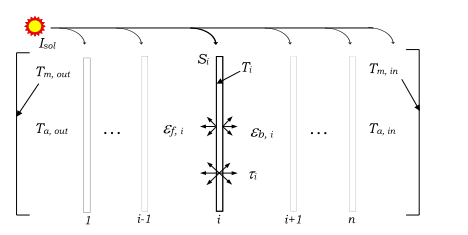
\includegraphics[width=0.9\textwidth, height=0.9\textheight, keepaspectratio=true]{media/image1827.svg.png}
\caption{Multi-layer fenestration analysis structure (ASHRAE 1311-RP) \protect \label{fig:multi-layer-fenestration-analysis-structure}}
\end{figure}

Equivalent layer fenestration model uses two-step analysis. First, the flux of absorbed solar radiation at each layer, S\(_{i}\), caused by the incident radiation flux, I\(_{sol}\), is determined using net radiation analysis. Second, an energy balance is applied at each layer, accounting for heat transfer and the known set of absorbed solar radiations S\(_{i}\) values, in order to solve for the set of layer temperatures, T\(_{i}\), and the corresponding heat fluxes. The fenestration model also accounts for the diathermanous shade layers in the longwave radiant exchange. The latter can be significant for shading layers. Glass is considered opaque with respect to longwave radiation.

\subsubsection{Equivalent Layer Optical Model}\label{equivalent-layer-optical-model}

The multilayer optical model is based on an algorithm originally developed by Edwards (1977) and extended by Wright and Kotey (2006). The algorithm models the interaction of incident solar radiation with a glazing system composed of any number of parallel, planar, specular glazing layers. The shading layers scatter portion of the incident solar radiation diffusely, and the model tracks the beam and diffuse components of solar radiation as they interact with a multi-layer system of glazing and shading layers. The conceptual arrangement for tracking beam and diffuse solar flux components is illustrated in Figure~\ref{fig:solar-analysis-of-the-multi-layer}.

Analysis yields beam-beam, beam-diffuse and diffuse-diffuse fluxes, providing full detail concerning the quantities of reflected, transmitted and absorbed radiation.

\begin{figure}[hbtp] % fig 114
\centering
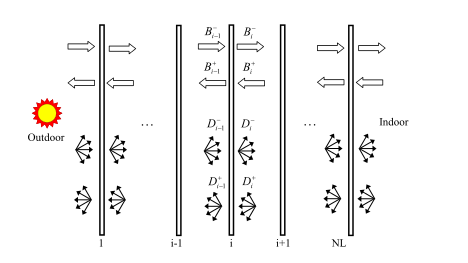
\includegraphics[width=0.9\textwidth, height=0.9\textheight, keepaspectratio=true]{media/image1829.svg.png}
\caption{Solar analysis of the multi-layer glazing/shading system showing beam and diffuse fluxes (ASHRAE 1311-RP) \protect \label{fig:solar-analysis-of-the-multi-layer}}
\end{figure}

The beam and diffuse characterization of solar radiation demands an expanded set of solar optical properties (Wright and Kotey 2006). The quantities of interest for single layer are shown in Figure~\ref{fig:twelve-solar-properties-assigned-at-each}.

where

$\tau$ ~~~ = ~~~~~~~~~ transmittance of a glazing or a shading layer, (-)

$\rho$ ~~~ = ~~~~~~~~~ reflectance of a glazing or a shading layer, (-)

$\varepsilon$ ~~~ = ~~~~~~~~~ thermal emissivity of a glazing or a shading layer, (-)

$\theta$ ~~ = ~~~~~~~~~ incident angle, (degree)

$\phi$ ~~ = ~~~~~~~~~ slat angle, (degree)

$\Omega$ ~~ = ~~~~~~~~~ profile angle, (degree)

\emph{J}~~~ = ~~~~~~~~~ radiosity of a layer surface, (W/m2)

\emph{T}~~~ = ~~~~~~~~~ temperature of a layer, (C)

Subscripts

\emph{f}~~~~ = ~~~~~~~~~ front side of a layer

\emph{b}~~~ = ~~~~~~~~~ back side of a layer

\emph{bb}~~ = ~~~~~~~~~ beam-beam optical property. Represents a fraction of the beam radiation incident at a given layer and leaves the layer without being scattered.

\emph{bd}~~ = ~~~~~~~~~ beam-diffuse optical property. Represents a fraction of the beam radiation incident at a given layer and leaves the layer diffusely

\emph{dd}~~ = ~~~~~~~~~ diffuse-diffuse optical property. Represents a diffuse radiation incident at a given layer and leaves the layer as diffuse

\emph{i~~~~ = ~~~~~~~~~} layer index, (-)

Superscripts

\emph{m}~~ = ~~~~~~~~~ represents material property (e.g., fabric material)

\emph{str}~ = ~~~~~~~~~ represents an apparent material structure property of roller blinds

\emph{w}~~~ = ~~~~~~~~~ represents an apparent wire property

\begin{figure}[hbtp] % fig 115
\centering
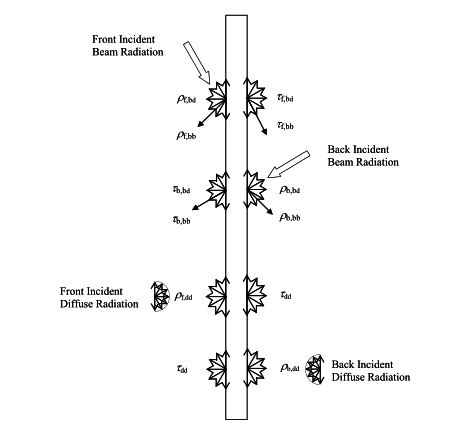
\includegraphics[width=0.9\textwidth, height=0.9\textheight, keepaspectratio=true]{media/image1830.svg.png}
\caption{Twelve solar properties assigned at each layer (ASHRAE 1311-RP) \protect \label{fig:twelve-solar-properties-assigned-at-each}}
\end{figure}

Each glazing or shading layer, in general, require eleven set of solar properties (Wright and Kotey 2006). Only beam-beam properties are needed for common glazing layers. Each shading layer is represented by a few set of component properties and geometries that are converted to the full set of layer optical and thermal properties by equivalent layer models (ASHRAE 1311-RP). The models also make account for off-normal incidence of solar radiation and can calculate the diffuse component from normal incidence values using numerical integration.

\subsubsection{Equivalent Layer Thermal Model}\label{equivalent-layer-thermal-model}

A surface energy balance is applied at each layer and the resulting set of equation is solved for layer temperatures and heat transfer fluxes. A schematic drawing of the multi-layer illustration and variables designation is shown in Figure~\ref{fig:radiosity-model-used-in-thermal-analysis-of}. The net radiation formulation based on the radiosities, Jf,i and Jb,i the radiant flux leaving the front and back surfaces of the i\(^{th}\) layer, respectively, is the used as a solution technique. The net radiant heat flux across a gap can be expressed as the difference between the radiosities of the bounding surfaces. The net radiation model analysis yields the layer temperatures and corresponding heat transfer coefficients that are used to determine U-factor and SHGC. The thermal analysis is done in ``ASHWAT\_Thermal'' routine.

\begin{figure}[hbtp] % fig 116
\centering
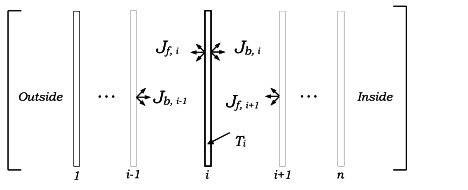
\includegraphics[width=0.9\textwidth, height=0.9\textheight, keepaspectratio=true]{media/image1831.svg.png}
\caption{Radiosity model used in thermal analysis of the multi-layer glazing/shading system (ASHRAE 1311-RP) \protect \label{fig:radiosity-model-used-in-thermal-analysis-of}}
\end{figure}

\subsubsection{Glazing Layer Analysis}\label{glazing-layer-analysis}

The Equivalent-Layer window model allows a wide range of options regarding the selection of glazing layers and gaps combinations. It also allows mixing glazing and shading layers in any sequence. For instance, it allows placing a venetian blind or a roller blind in between glazing layers. Only beam-beam solar properties at normal incidence, infrared transmittance and infrared emissivity are required for common glazing types. Off-normal solar properties at a given sun position are estimated by adjusting the normal incidence values in ``ASHWAT\_OffNormalProperties'' routine. The model assumes that the ratio between normal and off-normal transmittance is the same for the glazing layer in question and a reference piece of uncoated 6 mm glass with a moderate tint (ASHRAE 1311-RP). A similar procedure is used to convert solar reflectance from normal to off-normal.

\subsubsection{Gap Layer Analysis}\label{gap-layer-analysis}

Gaps can be specified as sealed, vented indoors or vented outdoors. The sealed gap is considered as enclosed cavity. Vented gaps is specified for inner and outer most gaps only and when the gas type is AIR. The vented gap model assumes that air flow at the perimeter of the window is not restricted. Any fill gas can be specified by molecular mass and thermo-physical properties of viscosity, specific heat and thermal conductivity. This is done by providing ``a'', ``b'' and ``c'' coefficients of the quadratic equation of the form, p = a + bT + cT\(^{2}\), where the T(K) is temperature and p is the property being evaluated. EnergyPlus has builtin-data available for common fill gas components including Air, Argon, Krypton and Xenon. Users specify CUSTOM gas by defining the coefficients as an input.

\subsubsection{Shade Layer Analysis}\label{shade-layer-analysis}

Equivalent layer fenestration model has a complete set of solar and longwave models for the four shading layer types: drapes, venetian blinds, roller blinds and insect screens developed under ASHRAE 1311-RP. And semi-empirical models are used to evaluate the off-normal properties of drape, roller blind and insect screen materials. The effective layer properties of venetian blinds and the effect of pleating in drapes are determined using a more fundamental net radiation scheme. The openness fraction, A\(_{o}\) and beam-beam solar transmittance at normal incidence, {$\tau$}\(_{bb}\) ($\theta = 0$), really represent a geometric quantity and it has been confirmed that they can be used interchangeably (ASHRAE 1311-RP). Openness is simply the fraction of a material, by area, that is open. In equivalent layer fenestration model, beam-beam transmittance at normal incidence (i.e., openness fraction), beam-diffuse transmittance and reflectance at normal incidence are required to characterize drapery fabric, roller blind and insect screen material. A conventional venetian blind in equivalent layer model can be characterized by specifying the geometry, solar reflectance and transmittance, and emissivity of the slats. The off-normal solar properties of drape, roller blind and insect screen materials were formulated based on measurements (ASHRAE 1311-RP). The longwave properties of the of the drape fabrics, roller blinds and insect screens can be calculated from the material emissivity and openness of the fabric (ASHRE 1311-RP). The optical model development for venetian blinds is presented by Yahoda and Wright (2004 and 2005), and Kotey et al. (2008).

\subsubsection{Drapes and Curtains}\label{drapes-and-curtains}

The off-normal optical properties of drapery fabric is determined from user specified optical properties at normal incidence ($\theta = 0$) using empirical correlations (Kotey et al., 2009a). The input data required to characterize drapery fabric are the beam-beam transmittance of the material at normal incidence {$\tau$}\(_{bb}\) ($\theta = 0$) = Ao, the beam-diffuse transmittance of the material at normal incidence {$\tau$}\(_{bd}\) ($\theta = 0$), and the beam-diffuse (total) reflectance of the material {$\rho$}\(_{bt}\) ($\theta = 0$). The off-normal properties are calculated as follows.

Off-normal Transmittance:

\begin{equation}
{\rm{\tau }}_{{\rm{bb}}}^{\rm{m}}\left( {\rm{\theta }} \right) = {\rm{\tau }}_{{\rm{bb}}}^{\rm{m}}{\rm{(\theta }} = {\rm{0)}} \cdot {\rm{co}}{{\rm{s}}^{\rm{b}}}\left( {\rm{\theta }} \right)
\end{equation}

\begin{equation}
{\rm{\tau }}_{{\rm{bt}}}^{\rm{m}}\left( {\rm{\theta }} \right) = {\rm{\tau }}_{{\rm{bt}}}^{\rm{m}}{\rm{(\theta }} = {\rm{0)}} \cdot {\rm{co}}{{\rm{s}}^{\rm{b}}}\left( {\rm{\theta }} \right)
\end{equation}

\begin{equation}
{\rm{b}} = {\left[ {\; - 0.5 \cdot \ln \;\left( {\;{{\left[ {{\rm{\tau }}_{{\rm{bb}}}^{\rm{m}}{\rm{(\theta }} = {\rm{0)}}\;{\rm{,}}\;\;{\rm{0}}{\rm{.01}}} \right]}^{\;\max }}\;} \right)\;\;,\;\;0.35\;} \right]^{\;\max }}
\end{equation}

\begin{equation}
{\rm{b}} = {\left[ {\; - 0.5 \cdot \ln \;\left( {\;{{\left[ {{\rm{\tau }}_{{\rm{bt}}}^{\rm{m}}{\rm{(\theta }} = {\rm{0)}}\;{\rm{,}}\;\;{\rm{0}}{\rm{.01}}} \right]}^{\;\max }}\;} \right)\;\;,\;\;0.35\;} \right]^{\;\max }}
\end{equation}

\begin{equation}
{\rm{\tau }}_{{\rm{bt}}}^{\rm{m}}\left( {\rm{\theta }} \right) = {\rm{\tau }}_{{\rm{bd}}}^{\rm{m}}\left( {\rm{\theta }} \right) + {\rm{\tau }}_{{\rm{bb}}}^{\rm{m}}\left( {\rm{\theta }} \right)
\end{equation}

The off-normal reflectance:

\begin{equation}
{\rm{\rho }}_{{\rm{bt}}}^{\rm{m}}\left( {\rm{\theta }} \right) = {\rm{\rho }}_{{\rm{bd}}}^{\rm{m}}\left( {\rm{\theta }} \right) = {\rm{\rho }}_{{\rm{bt}}}^{\rm{m}}\left( {{\rm{\theta }} = {\rm{0}}} \right) + \left( {{\rm{\rho }}_{{\rm{bt}}}^{\rm{m}}\left( {{\rm{\theta }} = 9{\rm{0}}^\circ } \right) - {\rm{\rho }}_{{\rm{bt}}}^{\rm{m}}\left( {{\rm{\theta }} = {\rm{0}}} \right)} \right) \cdot \left( {1 - {\rm{co}}{{\rm{s}}^{{\rm{0}}{\rm{.6}}}}\left( {\rm{\theta }} \right)} \right)
\end{equation}

\begin{equation}
{\rm{\rho }}_{{\rm{bt}}}^{\rm{m}}\left( {{\rm{\theta }} = {\rm{90}}^\circ } \right) = {\rm{\rho }}_{{\rm{bt}}}^{\rm{m}}\left( {{\rm{\theta }} = {\rm{0}}} \right) + \left( {{\rm{1}} - {\rm{\rho }}_{{\rm{bt}}}^{\rm{m}}\left( {{\rm{\theta }} = {\rm{0}}} \right)} \right)\;\left( {\,0.7{{\left( {\;{\rm{\rho }}_{}^{\rm{y}}} \right)}^{\;0.7}}} \right)
\end{equation}

The apparent yarn reflectance is given by:

\begin{equation}
{\rho ^y} = \frac{{\rho_{{\rm{bt}}}^{\rm{m}}\left( {{\rm{\theta }} = {\rm{0}}} \right)}}{{{\rm{1}} - \tau_{{\rm{bb}}}^{\rm{m}}\left( {{\rm{\theta }} = {\rm{0}}} \right)}} = \frac{{\rho_{{\rm{bt}}}^{\rm{m}}\left( {{\rm{\theta }} = {\rm{0}}} \right)}}{{{\rm{1}} - {{\rm{A}}_{\rm{o}}}}}
\end{equation}

The above set of equations for drapery fabrics are used subject to the condition that the solar absorptance of the fabric, at normal incidence, is not less than 1\% (ASHRE 1311-RP). The diffuse-diffuse material properties, for Equivalent layer window model, are determined using Rhomberg integration with 32 panels covering the range from $\theta = 0$ to $\theta = 90^{o}$ (ASHRAE 1311-RP). The subscript ``X'' stands for either front or back side of the layer.

\begin{equation}
  \tau_{x,dd}^{m} = 2\int_{\theta=0}^{\pi/2}\tau_{x,bt}^{m}\PB{\theta}\cos\theta\sin\theta d\theta
\end{equation}

\begin{equation}
  \rho_{x,dd}^{m} = 2\int_{\theta=0}^{\pi/2}\rho_{x,bt}^{m}\PB{\theta}\cos\theta\sin\theta d\theta
\end{equation}

The above set of equations for drapery fabrics apply to the full range of A\(_{o}\), fabric transmittance and fabric reflectance including that falls within the bounds of Keyes' (1967) fabric chart plus sheer fabrics (ASHRAE 1311-RP). The longwave thermal emissivity and thermal transmittances of drapery fabric are calculated using the following correlations and fabric openness fraction (Kotey et al. 2008).

\begin{equation}
{\varepsilon ^{\rm{m}}} = {\rm{0}}{\rm{.87}} \cdot \left( {{\rm{1 - }}{{\rm{A}}_{\rm{o}}}} \right)
\end{equation}

\begin{equation}
{\tau ^{\rm{m}}} = {\rm{1}} - {\rm{0}}{\rm{.95}} \cdot \left( {{\rm{1}} - {{\rm{A}}_{\rm{o}}}} \right)
\end{equation}

The optical and thermal properties determined using the above same sets of equations are equally valid for pleated drape shades (Kotey, et. al., 2009a). For pleated drape, the effective beam-beam and beam-diffuse solar properties are determined by tracking both radiation components, for a given incident angle, and interaction with a fabric pleated rectangular geometry shown in Figure~\ref{fig:geometry-used-for-pleated-drape-analysis}. The solar optical properties of the two different pleat planes are evaluated on the basis of the local solar incidence angle. Therefore, the effective layer properties are influenced not just by horizontal solar profile angle, {$\Omega$\(_{H}\), but also by incidence angle (ASHRAE 1311-RP).

\begin{figure}[hbtp] % fig 117
\centering
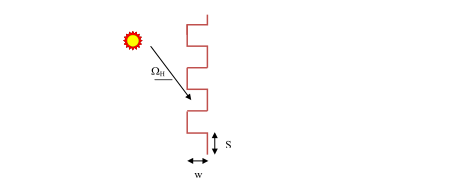
\includegraphics[width=0.9\textwidth, height=0.9\textheight, keepaspectratio=true]{media/image1844.svg.png}
\caption{Geometry used for Pleated Drape Analysis \protect \label{fig:geometry-used-for-pleated-drape-analysis}}
\end{figure}

The solar diffuse-diffuse and long-wave effective properties of the pleated drape are evaluated using a much simpler net-radiation analysis using conventional shape factors (Kotey, et. al., 2009a). Users can chose and apply the pleated drape model to any fabric and any degree of fullness (ASHRAE 1311-RP).

\subsubsection{Venetian Blinds}\label{venetian-blinds}

The effective shortwave optical and longwave optical properties of venetian blind layer is estimated using analytical models (Yahoda and Wright 2004, 2005; Kotey et al. 2008). The model requires properties of venetian blind slats and geometry of the slats shown in Figure~\ref{fig:geometry-and-properties-used-for-venetian}.

\begin{figure}[hbtp] % fig 118
\centering
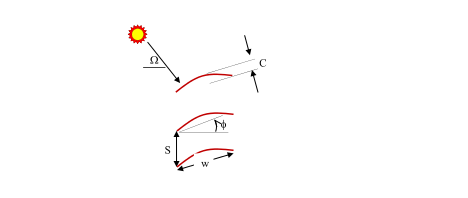
\includegraphics[width=0.9\textwidth, height=0.9\textheight, keepaspectratio=true]{media/image1846.svg.png}
\caption{Geometry and properties used for venetian blind analysis.~ The effective longwave properties are obtained for the layer knowing longwave properties of the slats. \protect \label{fig:geometry-and-properties-used-for-venetian}}
\end{figure}

The model assumes that venetian blind slats reflect and transmit solar radiation diffusely (ASHRAE 1311-RP). The same assumption is made regarding thermal radiation. The input data required to characterize a venetian blind are: front and back side reflectance and transmittance of the slat, geometry and infrared emissivity and transmittance of the slate. The effective optical properties of the venetian blind are determined by tracking beam and diffuse solar radiation through various interactions with slats positioned at a given slat angle. The model uses simple four-surface model if the slats are fully sunlit and a six-surface model if the slats are partially sunlit (ASHRAE 1311-RP). Slats are assumed to be thin and flat but a correction is applied to account for slat curvature effect (Kotey et al. 2008).

\subsubsection{Roller Blinds}\label{roller-blinds}

The off-normal properties of roller-blind are determined from solar properties of roller blind fabric measured at normal incidence ($\theta = 0$) using correlations (Kotey, et. al., 2009b). The off-normal properties for roller blind shades are calculated using the set equations given below:

\begin{equation}
{{\rm{\tau }}_{bb}}\left( {\rm{\theta }} \right) = \left\{ \begin{array}{l}{{\rm{\tau }}_{bb}}{\rm{(\theta }} = {\rm{0)}} \cdot {\rm{co}}{{\rm{s}}^{\rm{b}}}{\kern 1pt} \left( {\frac{{\rm{\theta }}}{{{{\rm{\theta }}_{{\rm{cutoff}}}}}} \cdot \frac{\pi }{2}} \right)\quad \theta  < {\theta_{CutOff}}\\0\quad \quad \quad \theta  \ge {\theta_{CutOff}}\end{array} \right.
\end{equation}

\begin{equation}
{\rm{b}} = {\rm{0}}{\rm{.6}} \cdot {\rm{co}}{{\rm{s}}^{{\rm{0}}{\rm{.3}}}}\left( {{{\rm{A}}_{\rm{o}}} \cdot \frac{{\rm{\pi }}}{{\rm{2}}}} \right)
\end{equation}

\begin{equation}
{{\rm{\theta }}_{{\rm{cutoff}}}} = {\rm{65}}^\circ  + \;\left( {{\rm{90}}^\circ  - {\rm{65}}^\circ } \right) \cdot \left( {{\rm{1}} - {\rm{cos}}\left( {{{\rm{A}}_{\rm{o}}} \cdot \frac{{\rm{\pi }}}{{\rm{2}}}} \right)} \right)
\end{equation}

\begin{equation}
{\rm{\tau }}_{{\rm{bt}}}^{}\left( {\rm{\theta }} \right) = {\rm{\tau }}_{{\rm{bt}}}^{}{\rm{(\theta }} = {\rm{0)}} \cdot {\rm{co}}{{\rm{s}}^{\rm{b}}}{\kern 1pt} \left( {\rm{\theta }} \right)
\end{equation}

\begin{equation}
b = \left\{ 
    \begin{array}{lc}
      0.133 \cdot \left( \rm{\tau}^{str} + 0.003 \right)^{-0.467} &\text{if} \left( 0 \le \rm{\tau}^{str} \le 0.33 \right) \\
      0.33 \cdot \left( 1 - \rm{\tau}^{str} \right)               &\text{if} \left( 0.33 < \rm{\tau}^{str} \le 1 \right)
    \end{array}
  \right.
\end{equation}

\begin{equation}
{\rm{\tau }}_{}^{{\rm{str}}} = \frac{{{\rm{\tau }}_{{\rm{bt}}}^{}\left( {{\rm{\theta }} = {\rm{0}}} \right) - {{\rm{\tau }}_{{\rm{bb}}}}\left( {{\rm{\theta }} = {\rm{0}}} \right)}}{{{\rm{1}} - {{\rm{\tau }}_{{\rm{bb}}}}\left( {{\rm{\theta }} = {\rm{0}}} \right)}}
\end{equation}

\begin{equation}
{\rm{\tau_{bt}}}\left( {\rm{\theta }} \right) = {\rm{\tau_{bd}}}\left( {\rm{\theta }} \right) + {\rm{\tau_{bb}}}\left( {\rm{\theta }} \right)
\end{equation}

The off-normal solar property calculation of roller blind is based on a set of correlations developed from measurement data using samples of commonly used commercially produced roller blind material openness range of 0.0 -- 0.14. Thus, these correlations are not applicable for shades with materials openness fraction exceeding 0.20. The mean solar reflectance of a roller blind material was found to be purely diffuse and unaffected by incidence angle and is given by:

\begin{equation}
{\rm{\rho }}_{{\rm{bt}}}^{}\left( {{\rm{\theta }} = {\rm{0}}} \right) = {\rm{\rho }}_{{\rm{bd}}}^{}\left( {{\rm{\theta }} = {\rm{0}}} \right) = {\rm{\rho }}_{{\rm{bt}}}^{}\left( {\rm{\theta }} \right) = {\rm{\rho }}_{{\rm{bd}}}^{}\left( {\rm{\theta }} \right)
\end{equation}

The diffuse-diffuse transmittance and reflectance are obtained by Rhomberg numerical integration. The longwave properties of roller blind material determined using the material property and the openness fraction (Kotey et al. 2008) as shown below:

\begin{equation}
{\varepsilon ^{{\rm{rb}}}} = {\rm{0}}{\rm{.91}} \cdot \left( {{\rm{1 - }}{{\rm{A}}_{\rm{o}}}} \right)
\end{equation}

\begin{equation}
{\tau ^{{\rm{rb}}}} = {\rm{1}} - {\rm{0}}{\rm{.95}} \cdot \left( {{\rm{1}} - {{\rm{A}}_{\rm{o}}}} \right)
\end{equation}

\subsubsection{Insect Screens}\label{insect-screens}

The empirical correlations formulated to obtain the effective off-normal solar and longwave properties of insect screens were based on measurements (Kotey et al. (2009a). Insect screen geometry is shown in Figure~\ref{fig:geometry-used-for-insect-screen-analysis}. The calculation of effective solar properties requires a set of properties measured at normal incidence: $\tau_{bb}$ ($\theta = 0$), $\tau_{bd}$ ($\theta = 0$) and $\rho_{bt}$ ($\theta = 0$).

\begin{figure}[hbtp] % fig 119
\centering
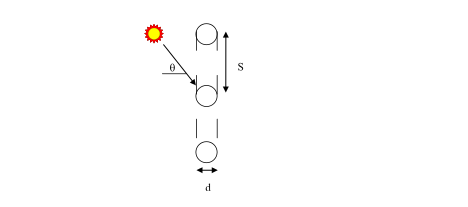
\includegraphics[width=0.9\textwidth, height=0.9\textheight, keepaspectratio=true]{media/image1857.svg.png}
\caption{Geometry used for insect screen analysis \protect \label{fig:geometry-used-for-insect-screen-analysis}}
\end{figure}

Openness can be determined by optical measurement at normal incidence, A\(_{o}\) = $\tau_{bb}$ ($\theta = 0$), but in the case of insect screens A\(_{o}\) can reliably be calculated knowing wire diameter (\emph{d}), and wire spacing (\emph{s}) as follows:

\begin{equation}
{A_o} = {\left( {1 - {d \mathord{\left/ {\vphantom {d s}} \right. } s}} \right)^2}
\end{equation}

The incidence angle beyond which direct beam transmission is cut off, {$\theta$}\(_{CutOff}\), can also be estimated purely from geometry and is given by:

\begin{equation}
{\theta_{CutOff}} = co{s^{ - 1}}\left( {{d \mathord{\left/ {\vphantom {d S}} \right. } S}} \right)
\end{equation}

The off-normal properties are calculated as follows.

\begin{equation}
{\tau_{bb}}\left( {\rm{\theta }} \right) = \left\{ \begin{array}{l}{\tau_{bb}}{\rm{(\theta }} = {\rm{0)}} \cdot {\rm{co}}{{\rm{s}}^{\rm{b}}}\left( {\frac{{\rm{\theta }}}{{{{\rm{\theta }}_{{\rm{cutoff}}}}}} \cdot \frac{\pi }{{\rm{2}}}} \right)\quad {\rm{\theta }} < {{\rm{\theta }}_{{\rm{cutoff}}}}\\0\quad \quad \quad \quad \quad \quad \quad \quad \quad \quad \quad \;\,{\rm{\theta }} \ge {{\rm{\theta }}_{{\rm{cutoff}}}}\end{array} \right.
\end{equation}

\begin{equation}
{\rm{b}} =  - {\rm{0}}{\rm{.45}}\;{\rm{ln}}\;\left( {{\rm{MAX}}\left( {{{\rm{\tau }}_{{\rm{bb}}}}\left( {{\rm{\theta }} = {\rm{0}}} \right){\rm{,}}\;{\rm{0}}{\rm{.01}}} \right)} \right)\; + \;{\rm{0}}{\rm{.1}}
\end{equation}

\begin{equation}
{\rm{\tau }}_{{\rm{bt}}}^{}\left( {\rm{\theta }} \right) = {\rm{\tau }}_{{\rm{bt}}}^{}{\rm{(\theta }} = {\rm{0)}} \cdot {\rm{co}}{{\rm{s}}^{\rm{b}}}\left( {\rm{\theta }} \right)
\end{equation}

\begin{equation}
{\rm{b}} =  - {\rm{0}}{\rm{.65}}\;{\rm{ln}}\;\left( {{\rm{MAX}}\left( {{{\rm{\tau }}_{{\rm{bt}}}}\left( {{\rm{\theta }} = {\rm{0}}} \right){\rm{,}}\;{\rm{0}}{\rm{.01}}} \right)} \right)\; + \;{\rm{0}}{\rm{.1}}
\end{equation}

\begin{equation}
{\rm{\tau }}_{{\rm{bd}}}^{}\left( {\rm{\theta }} \right) = {\rm{\tau }}_{{\rm{bt}}}^{}\left( {\rm{\theta }} \right) - {\rm{\tau }}_{{\rm{bb}}}^{}\left( {\rm{\theta }} \right)
\end{equation}

\begin{equation}
{\rm{\rho }}_{{\rm{bt}}}^{}\left( {\rm{\theta }} \right) = {\rm{\rho }}_{{\rm{bt}}}^{}\left( {{\rm{\theta }} = {\rm{0}}} \right) + \left( {{\rm{\rho }}_{{\rm{bt}}}^{}\left( {{\rm{\theta }} = 9{\rm{0}}^\circ } \right) - {\rm{\rho }}_{{\rm{bt}}}^{}\left( {{\rm{\theta }} = {\rm{0}}} \right)} \right) \cdot \left( {1 - {\rm{co}}{{\rm{s}}^{\rm{b}}}\left( {\rm{\theta }} \right)} \right)
\end{equation}

\begin{equation}
{\rm{b}} =  - {\rm{0}}{\rm{.45}}\;{\rm{ln}}\;{\left( {{{\rm{\rho }}^{\rm{w}}}} \right)^{}}
\end{equation}

\begin{equation}
{\rm{\rho }}_{}^{\rm{w}} = \frac{{{\rm{\rho }}_{{\rm{bt}}}^{}\left( {{\rm{\theta }} = {\rm{0}}} \right)}}{{{\rm{1}} - {\rm{\tau }}_{{\rm{bb}}}^{}\left( {{\rm{\theta }} = {\rm{0}}} \right)}}
\end{equation}

\begin{equation}
{\rho_{{\rm{bt}}}}\left( {{\rm{\theta }} = {\rm{90}}^\circ } \right) = {\rho_{{\rm{bt}}}}\left( {{\rm{\theta }} = {\rm{0}}} \right) + \left( {1 - {\rho_{{\rm{bt}}}}\left( {{\rm{\theta }} = {\rm{0}}} \right)} \right)\;\left( {{\rm{0}}{\rm{.35}}{\rho ^{\rm{w}}}} \right)
\end{equation}

The diffuse-diffuse material properties are obtained by Rhomberg numerical integration. The longwave properties of insect screen are given by expressions similar those formulated for drapery fabrics, and roller blinds (Kotey et al. 2008) is given by:

\begin{equation}
{\varepsilon ^{screen}} = {\varepsilon ^{\rm{w}}} \cdot \left( {{\rm{1  -  }}{{\rm{A}}_{\rm{o}}}} \right)
\end{equation}

\begin{equation}
{\tau ^{{\rm{screen}}}} = {\rm{1 - }}{\tau ^{\rm{w}}} \cdot \left( {{\rm{1  -  }}{{\rm{A}}_{\rm{o}}}} \right)
\end{equation}

The apparent wire material emissivity can be taken as $\varepsilon^w = 0.93$\ for common insect screens - screens with dark, rough, non-metallic wire surfaces. The corresponding infrared wire material transmittance is $\tau^w = 0.98$. A lower infrared emissivity can be used for screens constructed with shiny metallic wire. For example, to model stainless-steel wire mesh use $\varepsilon^w = 0.32$\ and $\tau^w = 0.81$.

\subsubsection{Integration with Heat Balance Method}\label{integration-with-heat-balance-method}

The solar model calculations are performed surface by surface following the existing structure of EnergyPlus's heat balance algorithm. The optical and thermal calculations are performed for each surface at each time step. The thermal model needs to be updated at each time step during the surface heat balance iteration. Thus, window thermal model is invoked during the surface heat balance but only once. This is consistent with the current EnergyPlus's window model inside surface heat balance iteration scheme. The equivalent layer window thermal model also has internal iteration scheme. The thermal model routine also requires the solar and shortwave radiation flux absorbed by each layer of a fenestration at each time step. The calculation of the absorbed radiation flux is performed using the existing scheme except that the optical properties are calculated by the equivalent layer optical model. The equivalent layer thermal model returns the temperatures and the fluxes at each layer.

\subsubsection{Equivalent Layer Window Solar Model}\label{equivalent-layer-window-solar-model}

The equivalent layer window solar model calculates the transmittance of the window and absorptance of each layer. Separate optical properties calculations are performed for exterior beam and diffuse radiations, and interior diffuse radiation (e.g., lighting and inter-reflected solar gain). The fractions for beam radiations depend on solar incident angle and hence updated for each time step. Diffuse radiation fractions are the same for all time steps unless the shade characteristics are altered; for instance, when the venetian blind slat angle is controlled. Otherwise, the diffuse fractions are constant for a given configuration and time step. The hub of the optical properties calculation routine for Equivalent Layer window model is the routine ``ASHWAT\_Solar''. For beam radiation, at each time step, first the normal incidence optical properties are modified for current incident angle. Using the off-normal properties, then the ASHWAT\_Solar routine sets up the coefficient matrix based on the net radiation concept to determine the effective absorptance of each layer and the window transmittance. The total intensity of shortwave radiation absorbed at each layer is determined by multiplying the incident solar radiation, reflected internal solar radiations, and internal shortwave source components by the appropriate absorbed fractions and summing them.

\subsubsection{Equivalent Layer Window Thermal Model}\label{equivalent-layer-window-thermal-model}

The equivalent layer thermal model is calculated only once for each time step. But the thermal model has internal iterative solutions scheme. During each time step, the procedure initially assumes that room air and means radiant temperatures are known. The surface heat balance loops through all zone surfaces while invoking the Equivalent Layer thermal model only once for each window surface at the first iteration. The window surfaces temperatures from the first iteration are used to complete the heat balances for the indoor (and implicitly the outdoor) face of each surface iteratively. Once indoor surface temperatures are calculated using the surface heat balance, the zone air temperature can be updated and the loads are predicted. Shaded fenestration in general do not have single inside temperature by virture their long-wave radiation transmittance. The equivalent layer window model accounts for this using effective emissivity of the composite layers derived for each fenestration (ASHRAE 1311-RP) as shown below:

\begin{equation}
{\varepsilon ^{eff}} = \sum\limits_{j = 0}^{nl} {\left[ {{\varepsilon_j} \cdot \prod\limits_{k = j{ + 1}}^{nl + {1}} {{\tau_k}} } \right]}
\end{equation}

where

\emph{$\varepsilon$\(^{eff}\)}~~ = ~~~~~~~~~ composite indoor (room-side) longwave emissivity, (-)

\emph{$\varepsilon$\(_{j}\)~~~ = ~~~~~~~~~} effective emissivity of layer j, (-)

\emph{$\tau$\(_{k}\)~~~ = ~~~~~~~~~} effective infrared transmittance of layer k (\{$\tau$\(_{1}\)} = 1)

\emph{nl~~~ = ~~~~~~~~~} number of layers in fenestration system (glazing and shade). Layers are numbered outside to inside (layer 1 is outermost, layer \emph{nl} is innermost).

Each equivalent layer window surafce yields net longwave radiant flux exchanged with the zone surfaces. Net longwave radiation exchange from the window to the zone is recast for a composite surface temperature calculation as follows:

\begin{equation}
{T^{eff}} = \sqrt[4]{{\frac{{{Q_{lw}}}}{{\sigma {\varepsilon ^{eff}}}}}} + {T_0}
\end{equation}

where

\emph{T\(^{eff}\)}~ = ~~~~~~~~~ inside surface temperature of the composite layer, °C (°F)

\emph{Q\(_{lw}\)}~~ = ~~~~~~~~~ infrared radiant gain from zone, W/m\(^{2}\) (Btu/h-ft\(^{2}\))

\emph{$\sigma$}~~~~ = ~~~~~~~~~ Stefan-Boltzmann constant, W/m\(^{2}\)-K\(^{4}\) (Btu/h-ft\(^{2}\)-R\(^{4}\))

\emph{T\(_{0}\)}~~~ = ~~~~~~~~~ Temperature of absolute zero, -273.15$^{\circ}$C (-459.67$^{\circ}$F)

Recalculating effective inside face window temperature may result in extra convection flux. The~ ``extra'' (Other) convective flux is computed; this is the gain in excess of that resulting from the standard surface heat balance model. The net other convection term \emph{QX} calculated below is added to the zone air heat balance (ASHRAE 1311-RP).

\begin{equation}
QX = {Q_{conv}} - hc \cdot ({T^{eff}} - {T_a})
\end{equation}

Where,

\emph{h\(_{c}\)~~~~ = ~~~~~~~~~} inside convective coefficient of the fenestration, W/m\(^{2}\)-K (Btu/h-ft\(^{2}\)-F)

\emph{Q\(_{conv}\)~= ~~~~~~~~~} total convective heat flux to zone from equivalent layer window thermal model, W/m\(^{2}\) (Btu/h-ft\(^{2}\)); includes open-channel gains and impact of inside surface convective coefficient

\emph{T\(_{a}\)~~~~ = ~~~~~~~~~} zone air temperature, °C (°F)

\subsubsection{References:}\label{references-2-009}

Edwards, D.K. 1977. Solar absorption by each element in an absorber-coverglass array, Technical Note, Solar Energy, Vol. 19, pp.~401-402.

Parmelee, G. V., and W. W. Aubele. 1952. The shading of sunlit glass: an analysis of the effect of uniformly spaced flat opaque slats, ASHVE Transactions, Vol. 58, pp.~377-398.

Farber, Erich A.; William A. Smith, C.W. Pennington, John C. Reed. 1963. Theoretical analysis of solar heat gain through insulating glass with inside shading. ASHRAE Transactions, Vol. 69, pp.393-405.

Rheault, S., and E. Bilgen. 1989. Heat transfer analysis in an automated venetian blind system, Journal of Solar Energy, Vol. 111 (Feb.), pp.~89-95.

Pfrommer, P., K. J. Lomas, and C. Kupke. 1996. ``Solar Radiation Transport through Slat-Type Blinds: a New Model and its Application for Thermal Simulation of Buildings,'' Solar Energy, Vol. 57, No. 2, pp.~77-91.

Rosenfeld, J.L.J., W. J. Platzer, H. Van Dijk, and A. Maccari. 2000. ``Modelling the Optical and Thermal Properties of Complex Glazing: Overview of Recent Developments'', Solar Energy, Vol. 69 Supplement, No. 1-6, pp.1-13.

Yahoda, D. S. and J. L. Wright. 2004. ``Methods for Calculating the Effective Longwave Radiative Properties of a Venetian Blind Layer,'' ASHRAE Transactions, Vol. 110, Pt. 1., pp.~463-473.

Yahoda, D. S. and J. L. Wright. 2005. ``Methods for Calculating the Effective Solar-Optical Properties of a Venetian Blind Layer,'' ASHRAE Transactions, Vol. 111, Pt. 1, pp.~572-586.

Yahoda, D. S. and J. L. Wright. 2004. ``Heat Transfer Analysis of a Between-Panes Venetian Blind Using Effective Longwave Radiative Properties,'' ASHRAE Transactions, Vol. 110, Pt. 1., pp.~455-462.

Huang, N.Y.T., J. L. Wright, M. R. Collins. 2006. ``Thermal Resistance of a Window with an Enclosed Venetian Blind: Guarded Heater Plate Measurements,'' ASHRAE Transactions, Vol. 112, Pt. 2. pp.~13-21.

Wright, J. L. 2008. ``Calculating Centre-Glass Performance Indices of Glazing Systems with Shading Devices,'' ASHRAE Transactions, Vol. 114, Pt. 2.

Wright, J. L., N. Y. T. Huang, and M. R. Collins. 2008. ``Thermal Resistance of a Window with an Enclosed Venetian Blind: A Simplified Model,'' ASHRAE Transactions, Vol. 114, Pt. 1.

Kotey, N. A., J. L. Wright, and M. R. Collins. 2008. ``Determining Longwave Radiative Properties of Flat Shading Materials,'' 33rd Annual SESCI / 3rd CSBC Conference Proceedings, Fredericton, NB.

Kotey, N.A., Wright, J.L., M. R. Collins. 2009a. ``Determination of Angle-Dependent Solar Optical Properties of Roller Blind Materials,'' drafted for submission to ASHRAE Transactions, Vol. 115, Pt. 1.

Kotey, N.A., Wright, J.L., M. R. Collins. 2009b. ``Determination of Angle-Dependent Solar Optical Properties of Drapery Fabrics,'' in review, ASHRAE Transactions, Vol. 115, Pt. 2.

Wright, John L., Charles S. Barnaby, Michael R. Collins, and Nathan A. Kotey. Improving Cooling Load Calculations for Fenestration with Shading Devices . ASHRAE 1311-RP, Final Report, February 11, 2009.
